\documentclass[12pt, a4paper, twoside]{report}
\usepackage{german, isolatin1, palatino}
\usepackage[dvips]{graphicx}
\usepackage{epsfig}
\usepackage{hyperref}
\usepackage{amsmath}
\usepackage{eurosym}
\bibliographystyle{alphadin}
\author{Christian R�diger, Christoph Reichenbach, Markus Weimer}
\title{Studienarbeit}

\pagestyle{headings}

\begin{document}
\begin{titlepage}

\maketitle
Verantwortlichkeit der Autoren f�r die Einzelnen Kapitel:
\begin{description}
\item[Markus Weimer] Kapitel
  \ref{laeufer_kapitel},\ref{aufgabe_kapitel}, \ref{mw_kapitel} und
  \ref{fazit_kapitel}
\item[Christoph Reichenbach] Kapitel \ref{jameson_kapitel}
\item[Christian R�diger] Kapitel \ref{cr_kapitel}
\end{description}

\end{titlepage}
\begin{abstract}
%mw
  Im Rahmen des Projektes L�ufer wurde w�hrend dieser Arbeit ein
  Mechatronisches System f�r den L�ufer entwickelt.  Dieses System
  schliesst drei Komponenten ein: Das Fahrerinformationssystem, eine
  Platine samt Software f�r die Entwicklung mechatronischer Systeme
  sowie eine auf CANBus basierende Kommunikationsstruktur.
  
  Die vorliegende Arbeit beschreibt die dabei getroffenen Design- und
  Produktentscheidungen vor dem Projektkontext.  Im ersten Kapitel
  soll zu diesem Zweck zun�chst ein �berblick �ber das Projekt L�ufer
  gegeben werden.  Darauf folgt im zweiten Kapitel eine sich aus dem
  Projekt ergebende Anforderungsdarstellund an die Mechatronik.  Diese
  beiden Kaptiel wurden in enger Zusammenarbeit mit den Projektleitern
  des L�ufers erstellt.  
  
  Die folgenden drei Kapitel beschreiben die drei Komponenten des
  mechatronischen Systems.  Dabei wird von der Anwenderschnittstelle
  �ber die Kommunikation der Ger�te bis zu den Ger�ten selbst
  vorgegangen.

  Im letzten Kapitel soll dann eine kurze Zusammenfassung und ein
  Ausblick gegeben werden.
%mw
\end{abstract}

% Inhaltsverzeichnis
\tableofcontents

% Abbildungsverzeichnis
\listoffigures

% Tabellenverzeichnis
\listoftables


\chapter{Das Projekt L�ufer}\label{laeufer_kapitel}
von: Markus Weimer
%\section{Das Projekt L�ufer}

Bei diesem Fahrzeug handelt es sich um ein von seinen Entwicklern
,,L�ufer'' getauftes Tandem, das sich durch die Vielzahl an
technischen Neuerungen auszeichnet, deren Entwicklung sich zwei Zielen
unterordnet: Reisetauglichkeit und Fahrspa�.

% Projekt
Entwickelt wird das Fahrzeug von Studenten der TU Darmstadt, TU
M�nchen sowie der FH Darmstadt in einem sehr interdisziplin�ren Team.
Beteiligt sind neben Maschinenbauern verschiedener Spezialisierungen
auch (Wirtschafts-)Informatiker, Textil- und Industrie-Designer.  Ziel
des Projektes ist die Entwicklung eines muskelgetriebenen
\emph{Reise}fahrzeugs f�r zwei Personen.  Der Schwerpunkt liegt hier
auf der Reisetauglichkeit, und nicht auf Dingen wie der theoretisch
erreichbaren Maximalgeschwindigkeit.  Neben der technischen
Herausforderung sind das Lernen in anderen Strukturen sowie die
intensive Zusammenarbeit mit Partnern aus Industrie und Forschung
Triebfedern f�r das Projekt.

% Technik 
Ein wichtiger Schritt, die Ziele Fahrspa� und Reisetauglichkeit zu
erreichen, ist die Gewichtsreduktion. So ist der L�ufer komplett aus
Aluminium und Kohlefaser gefertigt, was sein Gesamtgewicht auf ca.
$50kg$ reduziert.  Der L�ufer verf�gt im Gegensatz zu vielen anderen
muskelgetriebenen Fahrzeugen �ber eine Verkleidung. Diese dient zum
einen der Verbesserung der Aerodynamik, zum anderen aber auch als
Regenschutz.  Dies zusammen mit dem Antriebsstrang, auf den weiter
unten eingegangen werden soll, erm�glicht es zwei normal trainierten
Menschen mit dem Fahrzeug eine Durchschnittsgeschwindigkeit von ca.
$40km/h$ zu erreichen.  Dieser errechnete Wert bezieht sich allerdings
nicht etwa auf eine besonders ebene Route, sondern auf eine Strecke im
Odenwald rund um Darmstadt, also im Mittelgebirge.


% �berleitung zu Christian
Insbesondere im Bereich der Mechatronik, also der Verbindung von
Mechanik mit moderner Informationstechnologie, geht der L�ufer nicht
nur f�r Fahrrad-Verh�ltnisse neue Wege.



%%% Local Variables:
%%% mode: latex 
%%% TeX-master: "master"
%%% End:

\chapter{Aufgabenstellung}\label{aufgabe_kapitel}
von: Markus Weimer
\section{Anforderungen an die Mechatronik im L�ufer}

\cite{artikel}
\begin{description}
\item [Design]
\item [Erweiterbarkeit]
\item [Handhabbarkeit durch Ingenieure]
\item [Niedriger Stromverbrauch]
\item [Sicherheit]
\item [Fehlertoleranz]
\item [Sponsor-Barkeit]
\item [Verf�gbarkeit]
\item [Zeitlicher Rahmen des Projektes]
\end{description}


% Markus' Kapitel
\chapter{Fahrerinterface}\label{mw_kapitel}
von: Markus Weimer
\section{Aufgabenstellung}

Abbildung \ref{mw_seite} zeigt eine Seitenansicht des L�ufers.  Dabei
wurden die derzeit geplanten mechatronischen Komponenten markiert.\\
Im einzelnen sind dies:
\begin{figure}
  \center
  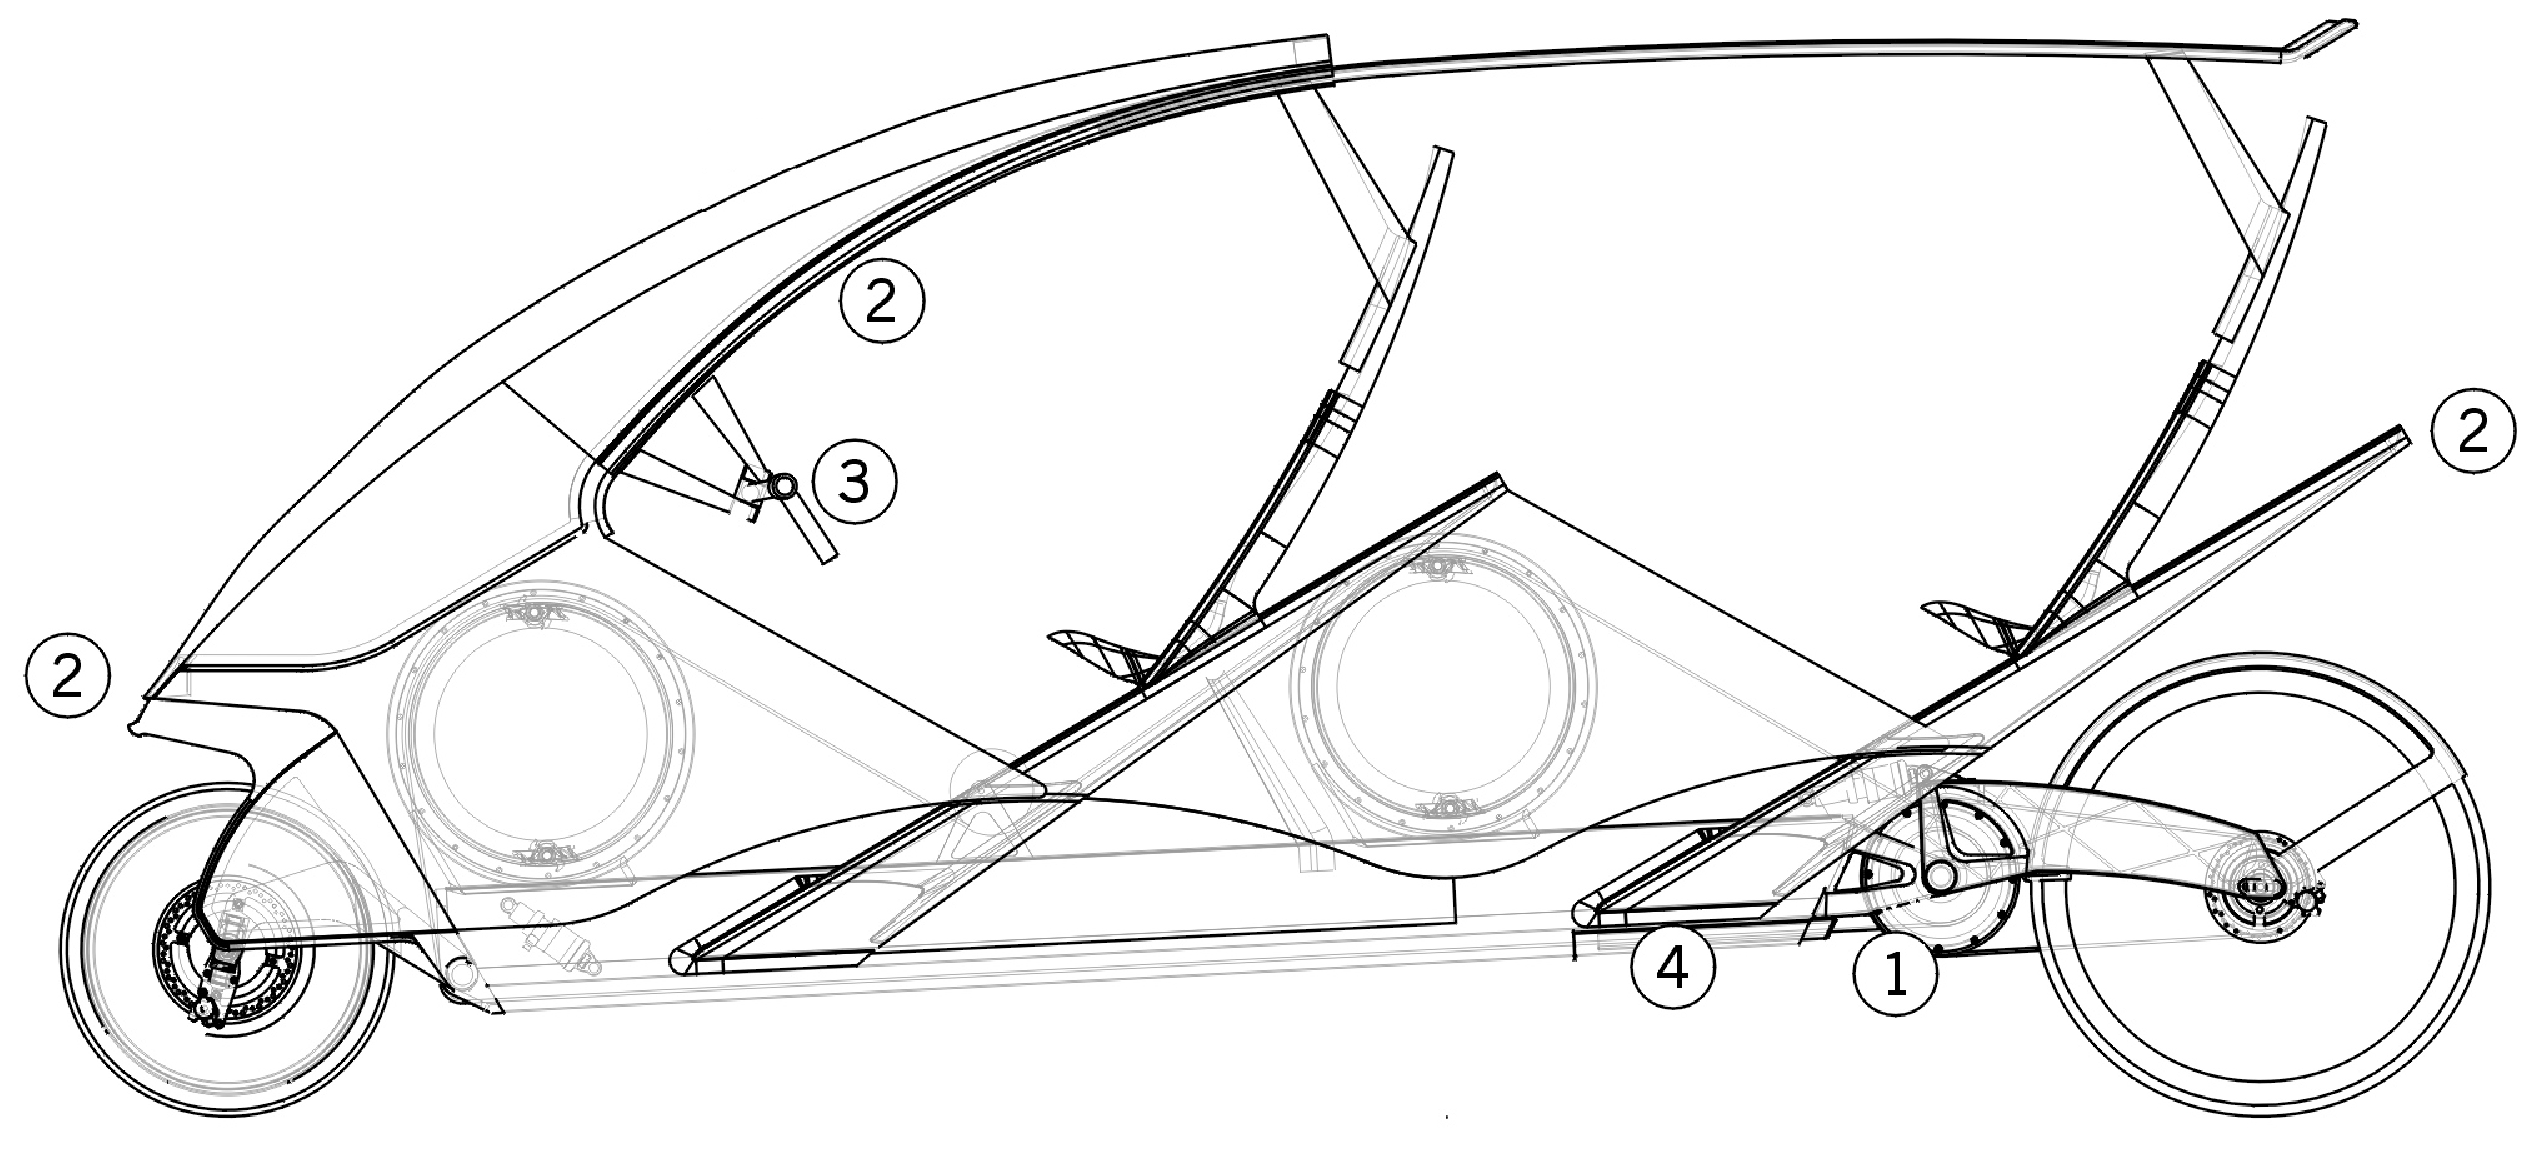
\includegraphics[width=13.5cm]{mw/bilder/seitenansicht.eps}
  \caption{Seitenansicht des L�ufers mit Markierungen der
    Mechatronischen Komponenten}
  \label{mw_seite}
\end{figure}

\begin{enumerate}
\item
  Antriebsstrang
\item
  Beleuchtungssystem 
\item
  Fahrerinformations-System
\item
  St�nder
\end{enumerate}

F�r die Zukunft sind weitere Komponenten m�glich und auch eingeplant.
Konkret angedacht wurde z.B. eine Anbindung eines GPS\footnote{Global
  Positioning System}-Systems �ber den CAN-Bus.  Diese mechatronischen
Komponenten des L�ufers verf�gen �ber etliche Parameter, die man als
Fahrer einstellen k�nnen will.  Als Beispiel sei hier nur der
Antriebsstrang genannt.  Dieser soll es dem Fahrer z.B. erm�glichen,
bei vollen Batterien und kurzer Strecke alleine elektrisch zu fahren,
und die Pedale ohne Widerstand zu benutzen.

Au�erdem gibt es Informationen �ber den aktuellen Zustand des
Fahrzeuges, die an den Fahrer weitergeleitet werden m�ssen.  Dies sind
zum einen Daten, wie man Sie auch vom normalen PKW kennt, wie z.B. die
aktuelle Geschwindigkeit.  Dazu kommen beim L�ufer spezielle
Informationen aus dem Antriebsstrang: Wie schnell kann man bei der
aktuell in den Pedalen abgegebenen Energie fahren? Oder, wie voll sind
die Batterien?  Diese Informationen m�ssen dem Fahrer in einer Art und
Weise zur Verf�gung gestellt werden k�nnen, die der Fahrsituation
angemessen ist.

Zus�tzlich m�chte der Entwickler einer mechatronischen Komponente
wahrscheinlich aufwendige Berechnungen, die sich aus den W�nschen des
Fahrers ergeben, in einer relativ komfortablen Hochsprache wie C/C++
programmieren, anstatt dies vergleichsweise umst�ndlich in Assembler
auf den Embedded Platinen zu tun.

Es ergeben sich also die folgenden Anforderungen an das
Fahrerinformationssystem des L�ufers:

\begin{description}
\item[Rechenleistung] Um die geforderten Berechnungen komfortabel in
  Hochsprachen durchf�hren zu k�nnen.
\item[Display] Um die Informationen f�r den Fahrer darzustellen. Dies
  ersetzt das Armaturenbrett eines PKW.
\item[Interaktion] Um die teilweise sehr umfassenden
  Einstellungsm�glichkeiten des Fahrzeugs ausnutzen zu k�nnen.
\end{description}

Diese Aufgaben lassen sich in hervorragender Weise von aktuellen
Taschencomputern, sogenannten PDAs\footnote{PDA: Personal Digital
  Assistent, zu Deutsch etwa: Pers�nlicher Digitaler Assistent.}
erf�llen. Diese Ger�te, insbesondere die neuerer Bauart, verf�gen �ber
gen�gend Rechenleistung, um die Aufgaben innerhalb des L�ufers
bew�ltigen zu k�nnen.  Zus�tzlich sind diese Ger�te sehr stark auf den
sorgsamen Umgang mit Energie optimiert, was in einem Fahrzeug, da�
seine Energie ausschlie�lich aus der Muskelkraft seiner Fahrer
bezieht, nat�rlich von besonderem Interesse ist.  Au�erdem sind sie
in gro�en St�ckzahlen kommerziell verf�gbar, was den Preis f�r den
einzelnen PDA stetig sinken l��t.

Aufgabe im Bereich des Fahrerinformationssystems ist es also
einerseits, einen geeigneten PDA auszuw�hlen und diesen andererseits
durch das Erstellen zus�tzlicher Software f�r das Projekt nutzbar zu
machen.  Diese Software ist vor allem ein Kommunikationssystem
zwischen PDA und den im Fahrzeug verteilten Komponenten.  Dies ist
n�tig, da im PDA-Bereich zwar die aus dem PC-Markt bekannten
Schnittstellen und Kommunikationsprotokolle zur Verf�gung stehen,
diese jedoch im Allgemeinen bei mechatronischen Komponenten nicht
verf�gbar sind.

Diese Kommunikation mu� f�r den Entwickler einer mechatronischen
Komponente f�r den L�ufer m�glichst einfach zu handhaben sein.  Diese
Forderung ergibt sich aus der Arbeitsteilung zwischen den
verschiedenen Disziplinen im Projekt, im konkreten Fall also zwischen
Informatik und Maschinenbau.  Innerhalb dieser Arbeit soll ein
Kommunikationssystem entworfen und auch implementiert werden, das es
den Ingenieuren im Projekt erm�glicht, ihr Fachwissen auf die
Fahrzeuglogik des L�ufers zu �bertragen, ohne zu tief in die Details
der Implementierung eines Kommunikationssystems einsteigen zu m�ssen.

Neben diesen Anforderungen der Entwickler mechatronischer Komponenten
soll aber gerade bei der Auswahl des PDAs der sp�tere Nutzer des
L�ufers und seine W�nsche Ber�cksichtigung finden. Dieser w�nscht sich
von einem solchen Ger�t einen Mehrfachnutzen.  Es soll also sowohl als
,,Bordcomputer'' des L�ufers fungieren k�nnen, als auch ein
vollwertiger PDA sein.

Im folgenden soll zun�chst die Entscheidung f�r einen speziellen PDA
transparent gemacht werden.  Daraufhin wird die
Kommunikations\-schnittstelle f�r die Entwickler mechatronischer
Komponenten f�r den L�ufer beschrieben.

Im Bereich der Projektarbeit ergeben sich nat�rlich auch
Anforderungen, die sich nicht so direkt aus theoretischen Erw�gungen
ableiten lassen k�nnen.  Viele Anforderungen werden erst und immer
wieder im Gespr�ch mit den Projektteilnehmern aus anderen
Fachgebieten, wie z.B. dem Maschinenbau oder dem Industriedesign,
deutlich.  Ergebnisse dieser Anforderungen sind unter anderem der so
genannte DebugTreiber, auf den am Ende dieses Kapitels exemplarisch
f�r die interdisziplin�re Zusammenarbeit innerhalb des Projektes
eingegangen werden soll.


\newpage
\section{Auswahl des PDA}
\subsection{Anforderungen}
Die Anforderungen an den PDA ergeben sich aus den Anforderungen an die
gesamte Mechatronik sowie das Fahrerinformationssystem im speziellen.
Sie lassen sich in Anforderungen an die PDA Systemsoftware und
Anforderungen an die PDA-Hardware gliedern, was im folgenden geschehen
soll.  Diese Gliederung ist hilfreich, da sich auch der PDA-Markt sehr
gut nach der Systemsoftware der PDAs unterteilen l��t.  Dies wird
weiter unten zur Vorauswahl des PDAs ausgenutzt.

\subsubsection{Anforderungen an die Software}
\begin{description}
\item[Multitasking] Diese Anforderung ergibt sich unmittelbar aus der
  Forderung an die gesamte Mechatronik, erweiterbar zu sein.  Ein PDA
  ohne Multitasking w�rde aber bei jeder Erweiterung des Systems einen
  Eingriff in die sicherheitsrelevante Fahrsoftware des L�ufers
  erfordern, was z.B. beim Einf�gen eines GPS\footnote{GPS=Global
    Positioning System} basierten Navigationssystems nicht
  w�nschenswert ist.
  
\item[GUI-Flexibilit�t] Das Projekt L�ufer geht in vielen Bereichen
  einen designorientierten Weg, der nicht unerheblich zu dem gro�en
  Erfolg des L�ufers in der �ffentlichkeit sowie beim Aufbau von
  Industrie-Partnerschaften beigetragen hat.  Auch im Bereich der
  graphischen Interaktion mit dem System soll dieser Design
  orientierte Weg m�glich sein, um den L�ufer als ,,rundes Produkt''
  entwickeln zu k�nnen.
  
  Also ist bei der Auswahl eines PDA samt zugeh�riger Software darauf
  zu achten, da� man im Bereich der Gestaltung des
  GUI\footnote{GUI=Graphical User Interface, zu Deutsch: Graphische
    Benutzer Schnittstelle}  gr�sst\-m�gliche Freiheiten hat.

  
\item[Programmierung] Die Programmierung des PDA sollte einfach sein,
  wobei mit ,,einfach'' in diesem Fall gemeint ist, da� die
  Entwicklung f�r den PDA sich m�glichst wenig von der Entwicklung f�r
  einen PC unterscheiden sollte.  Dies ist notwendig, da die sp�teren
  Nutzer unserer Software wahrscheinlich schon �ber Erfahrungen in der
  Programmierung von PCs verf�gen und deren Lernaufwand ja so niedrig
  wie m�glich zu halten ist.
  
  Au�erdem erm�glicht eine solche Vorgehensweise idealerweise die
  Entwicklung der Software auf einem PC, um sie dann sp�ter ohne
  gro�e Umst�nde einfach auf den PDA �bertragen zu k�nnen.  Dies
  spart inbesondere vor dem Projekthintergrund und der verteilten
  Produktentwicklung erhebliche Kosten f�r die Beschaffung von PDAs
  f�r die einzelnen Entwicklerteams in Darmstadt und M�nchen.
  
\item[Dokumentation und Support] Da die Entwicklung der Software �ber
  diese Studienarbeit hinaus von weiteren Entwicklern fortgesetzt
  werden soll, ist eine gute Dokumentation und ein umfassender Support
  der verwendeten Werkzeuge, Bibliotheken und Compiler mehr als
  w�nschenswert.
  
  Aus den selben Gr�nden ist es n�tig, auf eine m�glichst
  ,,langlebige'' Plattform zu setzen, die sich nicht innerhalb des
  Projektes st�ndig ver�ndert, bzw. f�r deren eingesetzte Version man
  in Zukunft wom�glich keine Entwicklungstools mehr erwerben kann.
  
\end{description}


\subsubsection{Anforderungen an die Hardware}
Auch an die Hardware eines PDA f�r den Einsatz in einem Fahrzeug
stellen sich besondere Anforderungen, die hier erl�utert werden
sollen.

\begin{description}
\item[Display] Beim Display eines PDA f�r den Einsatz im L�ufer gibt
  es zwei Dinge zu beachten: zum einen sollte es sich um ein
  Farbdisplay handeln und zum anderen sollte es vor allem unter all
  den Lichtbedingungen, in denen der L�ufer unterwegs sein wird, gut
  ablesbar sein.
  
  Die Forderung nach einem Farbdisplay ergibt sich zum einen aus der
  Design-Orientierung des Projektes und der Anforderung nach
  GUI-Flexibilit�t.  Zum anderen aber auch aus der �berlegung, da�
  man zum der Fahrsituation angemessenen Darstellen von z.B.
  Warnmeldungen wohl kaum auf Farbe verzichten kann.  So lassen sich
  durch Farbe gerade im Fahrbetrieb wichtige Informationen
  hervorheben, wie man das z.B. vom PKW mit seinen \emph{roten}
  Warnleuchten f�r wichtige Meldungen her kennt.
  
  Die Anzeigeeigenschaften des Display bei sehr extremen
  Lichtverh�ltnissen sind f�r den L�ufer entscheidend.  Das Display
  mu� bei allen Fahrsituationen m�glichst gut ablesbar sein, um den
  Fahrer �ber den aktuellen Zustand seines Fahrzeuges zu informieren.
  Zu den kritischen Lichtverh�ltnissen geh�rt dabei weniger die Nacht,
  da alle modernen PDAs �ber eine Leistungsf�hige Beleuchtung
  verf�gen.  Wesentlich wichtiger ist das Verhalten w�hrend der
  D�mmerung und bei starkem Sonnenschein.  Beides stellt einige
  Display-Konzepte bei heute markt�blichen PDAs vor gro�e Probleme.
  
  Als Beispiel sei hier die inverse Hintergrundbeleuchtung der PDAs
  des Herstellers Palm genannt, die zwar bei absoluter Dunkelheit
  hervorragende Dienste leistet, bei D�mmerung aber zu Unlesbarkeit
  des Displays f�hrt.
  
\item[Optik] Ein ebenfalls nicht zu untersch�tzender, wenn auch nur
  subjektiv zu beurteilender, Bereich ist die optische Erscheinung des
  PDA.  Dies spielt aus technischer Sicht nat�rlich nur eine
  untergeordnete Rolle, wird jedoch im Projektkontext bedeutsam, da
  einige Elemente des L�ufers nur unter �sthetischen Gesichtspunkten
  zu Stande gekommen sind.  Da sich unsere Arbeit in das Projekt
  integriert, m�ssen wir diesem Gesichtspunkt ebenfalls Bedeutung
  zumessen.
  
  Ein objektiv nachpr�fbarer Bereich der Optik ist die Bauform.  F�r
  den Einsatz im L�ufer kommen nur sogenannte Stift-PDAs in Frage, bei
  denen das Display hochkant steht und die Eingabe �ber einen Stift
  erfolgt.  Nur diese Bauform l��t sich vern�nftig in das
  Fahrzeug-Cockpit des L�ufers integrieren.
  
\item[Anschlu�m�glichkeiten] Da das Projekt L�ufer eines mit
  ausser\-gew�hnlicher Dynamik ist, ist die Anschlussvielfalt an einem
  PDA im L�ufer ein wesentliches Argument, um sich sp�tere
  Erweiterungen nicht durch einen zu beschr�nkten PDA zu verbauen.
  
  Die Mindestanforderung in diesem Bereich ist eine RS232\footnote{Im
  PC-Bereich auch h�ufig nur ,,serielle Schnittstelle'' genannt.}
  Schnittstelle, da �ber diese die Verbindung zu einer unserer
  Platinen hergestellt wird.  Diese Platine verbindet dann den PDA mit
  dem CAN-Bus. [FIXME Referenz auf Jameson]
\end{description}


\subsection{Auswahl der Systemsoftware}
Der PDA Markt l��t sich, wenn man die diversen geschlossenen Systeme
au�er Acht l��t, nach den Betriebssystemen PalmOS, WindowsCE und
Linux aufgliedern.  Die Ebenfalls noch angebotenen PDAs der Firma
PSION finden hier keine Beachtung, da deren Vermarktung und
Weiterentwicklung mittlerweile eingestellt wurde.  Au�erdem pa�t
deren Tastatur-Orientiertes Design nicht in das Konzept des
Cockpit-Entwurfs f�r den L�ufer.

Diese Einteilung nach Betriebssystem lieferte eine erste
Kategorisierung des PDA-Marktes.  Da zu jedem System relativ viele
verschiedene PDAs am Markt sind, war die Entscheidung anhand der
Software die erste, die zu treffen war.

Im folgenden sollen die einzelnen Systeme samt ihrer f�r das Projekt
relevanten Eigenschaften vorgestellt werden, um sich unter diesen drei
Systemen f�r eins zu entscheiden, da� die Software-Seitigen
Voraussetzungen f�r einen Einsatz im L�ufer mitbringt.
\begin{description}
\item[PalmOS] Dieses System wurde von der Firma 3Com entwickelt und
  zu\-n�chst ausschlie�lich auf deren PDAs, den sogenannten
  ,,PalmPilots'' eingesetzt.  Mittlerweile hat es PalmOS zur
  Marktf�hrerschaft gebracht und ist auch auf den Ger�ten von
  Herstellern wie Sony, Handspring und anderen zu finden.
  
  Als erstes wurden dann auch Ger�te mit diesem System ins Auge
  gefa�t.  Bei diesen Ger�ten kann man aufgrund der gro�en
  Verbreitung mit einer guten Akzeptanz seitens der Nutzers des
  L�ufers rechnen.  Auch wird ein eventueller Kunde mit hoher
  Wahrscheinlichkeit schon �ber ein solches Ger�t verf�gen.
  
  Ein ,,Palm IIIx'' wurde dann auch Basis eines ersten Versuchs der
  Mechatronik, der im Rahmen einer Studienarbeit von J�rn
  Schlingen\-siepen\cite{Schlinge} stattfand.  Im Rahmen dieser Arbeit
  wurde die grund\-s�tzliche M�glichkeit der Anbindung eines solchen
  Ger�tes an den CANBus untersucht und auch best�tigt.
  
  Allerdings verf�gt PalmOS in seiner jetzigen Version nicht �ber
  Multitasking, was einen Einsatz im L�ufer nicht erm�glicht, da dies
  die geforderte Erweiterbarkeit nicht in dem Masse sicherstellt, wie
  dies gefordert war.
  
  Im Bereich der Graphischen Gestaltung des Fahrerinterface erwiesen
  sich die verf�gbaren Ger�te dieser Bauart als recht eingeschr�nkt,
  da sie weder �ber eine anpa�bare Bibliothek von Oberfl�chenelementen
  noch �ber gen�gend Rechenleistung verf�gen, diese selbst zu
  ,,malen''.  Dies ist bei einem System wie PalmOS jedoch kein
  Design-Fehler, sondern schl�gt sich z.B. in der �berwiegend
  konstanten und guten Bedienbarkeit der Software f�r diese PDAs
  nieder.  Diese an sich gute Eigenschaft wird aber vor dem
  Hintergrund unserer Aufgabe hinderlich.
  
  Die Programmierung eines PalmOS-PDAs erfolgt mit speziellen Tools.
  Allerdings haben sich diese PDAs im Laufe der Zeit so weit
  verbreitet, da� mehrere alternative Programmierumgebungen und
  Compiler zur Verf�gung stehen.  Auch hat diese Verbreitung zu einer
  guten und frei verf�gbaren Dokumentation der
  Programmierschnittstelle und -Praktiken f�r diese Ger�te gef�hrt.
  
\item[Windows CE / Pocket PC] PDAs mit diesem System von Microsoft
  zeichnen sich durch Ihre leistungsf�hige Hardware aus.  So ist es
  bei diesen Ger�ten nicht selten, einen Prozessor mit deutlich mehr
  als 200MHz Taktfrequenz vorzufinden.
  
  Auch verf�gt Windows CE �ber Multitasking, eine permanent im
  Hintergrund laufende Fahrsoftware ist also mit diesem System
  realisierbar.
  
  Die Graphische Oberfl�che ist sehr an die Desktop-Versionen von
  Windows angelehnt.  Die Flexibilit�t bei der Gestaltung einer
  Oberfl�che f�r die L�ufersoftware ist auch unter Ber�cksichtigung der
  Einschr�nkung durch die Festlegung auf eine Entwicklungsumgebung
  schon alleine deshalb gro�, weil die Ger�te �ber so gro�e
  Leistungsreserven verf�gen.  Diese erm�glichen im Prinzip sogar eine
  komplett ,,gemalte'' Oberfl�che, auch wenn diese recht viel Speicher
  verbraucht.
  
  Die Programmierung des Systems erfolgt mittels der bekannten
  Microsoft-Tools wie z.B. Visual C++.  Diese sind schon alleine
  aufgrund Ihrer Verbreitung bestens Dokumentiert.  Allerdings ist
  WindowsCE genauso wie PalmOS ein reines PDA-System, so da� die
  Entwicklung f�r diese PDAs mit diesen speziellen Tools erfolgen mu�
  und zum Testen der Software ein Emulator zum Einsatz kommt.


\item[Linux] Linux ist im gesamten PDA und Embedded-Bereich ein
  ziemlicher Neuling, allerdings mit steigender Verbreitung.  Dies ist
  vor allem auf die gro�e Flexibilit�t dieses Systems zur�ckzuf�hren.
  
  Linux verf�gt nat�rlich auch auf dem PDA �ber echtes Multitasking.
  Schlie�lich kommt der selbe Kernel und die selbe Systemsoftware zum
  Einsatz wie auf den anderen Plattformen, auf denen es eine
  Implementierung dieses freien Betriebssystems gibt.
  
  Diese Gleichheit in der Software bringt Linux auf dem PDA eine gro�e
  Flexibilit�t, da direkt die gesamte Software, die es f�r Linux gibt,
  verf�gbar ist.  Dies betrifft insbesondere die Bibliotheken f�r
  Entwickler.  So existieren z.B. mehrere GUI-Bibliotheken, die noch
  dazu auf verschiedenen Wegen mit der Hardware kommunizieren k�nnen.
  Dies soll nur ein Beispiel f�r die Auswahl an M�glichkeiten sein,
  die f�r unsere Anwendung geradezu ideal ist.
  
  Aus der identischen Software auf PC/Workstation und PDA folgt aber
  auch, da� man Software f�r den PDA unter Ber�cksichtigung einiger
  Randbedingungen auf dem PC entwickeln und testen kann.  Dabei kann
  auf einen Emulator der PDA-Hardware verzichtet werden.  Dies macht
  es m�glich, da� Entwickler Software auf Ihrem PC entwickeln und mit
  diesem testen, die dann sp�ter durch ein �bersetzen f�r den
  PDA\footnote{Diesen Vorgang nennt man im Allgemeinen
    ,,crosscompiling''} auf diesen portiert werden kann.
  
  Diese gro�e Flexibilit�t zieht allerdings auch einen entscheidenden
  Nachteil nach sich: Nahezu jeder Entwickler f�r Linux-basierte
  Embedded Systems arbeitet mit seinem eigenen Set an Tools,
  Bibliotheken und Compilern.  Daraus folgt, da� es keine gro�e
  Entwicklergemeinde gibt, die alle mit den selben Tools arbeiten, was
  zu einer Un�bersichtlichkeit der Dokumentation f�hrt.  Dieser
  Umstand wird allerdings durch die Gleichheit des Systems zu dem auf
  PCs teilweise wieder ausgeglichen.


  
\item[Entscheidung] Letztlich war die Entscheidung zwischen Windows
  CE, heute PocketPC, und Linux zu treffen.  PalmOS ist wegen der
  fehlenden Multitasking-F�higkeit f�r unsere Aufgabe ungeeignet.
  
  Wir haben uns letztendlich f�r Linux entschieden, um uns die gr��te
  Flexibilit�t zu sichern.  Dies betrifft nicht nur die oben schon
  ausgef�hrte Auswahl an GUI-Bibliotheken, sondern auch die
  M�glichkeit im Falle der Notwendigkeit selbst am Betriebssystem Hand
  anlegen zu k�nnen.  Da wir ein klassisches Embedded System durch
  einen handels�blichen PDA ersetzten, war zu Beginn nicht klar,
  welche Probleme dabei auftreten k�nnen.  Und mit einem
  unab�nderlichen Betriebssystem waren diese Probleme eventuell nicht
  l�sbar.
  
  Zus�tzlich ist es mit einem Linux-PDA m�glich, Software auf PCs zu
  entwickeln und zu testen, ohne da� dazu ein PDA oder gar ein
  Emulator n�tig ist.
\end{description}
\begin{table}
  \caption{�bersicht �ber die verschiedenen PDA-Betriebssysteme}
  \label{mw_pda_os_tabelle}
  \begin{center}
    \begin{tabular}{|c|c|c|c|}
      \hline
      \emph{Anforderung} & \emph{PalmOS} & \emph{WindowsCE} & \emph{Linux} \\
      \hline
      \emph{Multitasking} &$\circ$ &$\bullet$ & $\bullet$\\
      \hline
      \emph{GUI-Flexibilit�t} &$\circ$ &+ & ++\\
      \hline
      \emph{Programmierung} &$\circ$ &+&++\\
      \hline
      \emph{Dokumentation und Support} &++ &+ &+\\
      \hline
    \end{tabular}
  \end{center}
\end{table}



\subsection{Auswahl der Hardware\label{mw_pda_uebersicht}}
Im folgenden sollen kurz die PDAs beschrieben werden, die f�r das
Projekt in Frage kamen, und die in folge dessen auch n�her gepr�ft
wurden.

Da der Markt f�r Linux-basierte PDAs sehr in Bewegung ist, kann und
soll hier keine vollst�ndige und insbesondere keine aktuelle �bersicht
gegeben werden.  Ein guter Anlaufpunkt f�r eine solche ist die
Homepage von Linuxdevices\footnote{http://www.linuxdevices.com}.

\begin{table}
  \caption{�bersicht �ber die verschiedenen Linux-f�higen PDAs}
  \label{mw_pda_tabelle}
  \begin{center}
    \begin{tabular}{|c|c|c|c|c|}
      \hline
      \emph{Anforderung} & \emph{Display} & \emph{Optik} & \emph{Anschlu�m�glichkeiten} & \emph {Verf�gbarkeit}\\
      \hline
      \emph{VR3}         & -- & 0 & 0 & + \\
      \hline
      \emph{Yopy}        &  + & + & 0 & -- \\
      \hline
      \emph{Helio}       & -- & --& 0 & + \\
      \hline
      \emph{Cassiopeia}  &  + & + & + & -- \\
      \hline
      \emph{Zaurus}      & ++ & + & + & (-) \\
      \hline
      \emph{IPAQ}        & ++ & ++& + & + \\
      \hline
    \end{tabular}
  \end{center}
\end{table}


\begin{description}
\item[Agenda VR3] Diesem PDA, der in Abbildung \ref{mw_agenda} zu
  sehen ist, geb�hrt die Ehre des ,,first-to-market''-Ger�tes im
  Bereich Linux-PDAs, da es Agenda Computing als erstes gelang, einen
  endkundentauglichen PDA mit Linux als Betriebssystem in die L�den zu
  bringen.
  \begin{figure}
    \center
    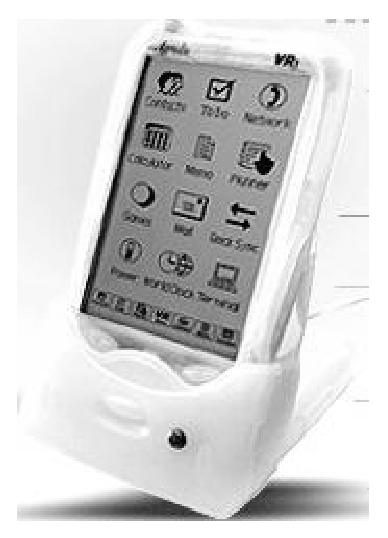
\includegraphics[width=7.0cm]{mw/bilder/agenda.eps}
    \caption{Der Agenda VR3}
    \label{mw_agenda}
  \end{figure}
  
  Leider gab es zum Zeitpunkt der Entscheidung noch keine
  Farb-Variante dieses Ger�ts. Farbe ist aber in einer
  Design-orientierten Entwicklung wie dem L�ufer ein absolutes Mu�.
  
\item[G.Mate Yopy] Abbildung \ref{mw_yopy} zeigt diesen PDA, der lange
  Zeit als Mythos durch die diversen News-Seiten und -Foren des
  Internet geisterte. Ihm wurde am ehesten zugetraut, der erste
  brauchbare PDA mit Linux als Betriebssystem zu sein.  Diese Hoffnung
  der Linux-Enthusiasten wurde nicht zuletzt durch die Pr�sentation
  des Yopy auf der Cebit 2000 durch den damaligen G.Mate-Partner
  Samsung gen�hrt.

  \begin{figure}
    \center
    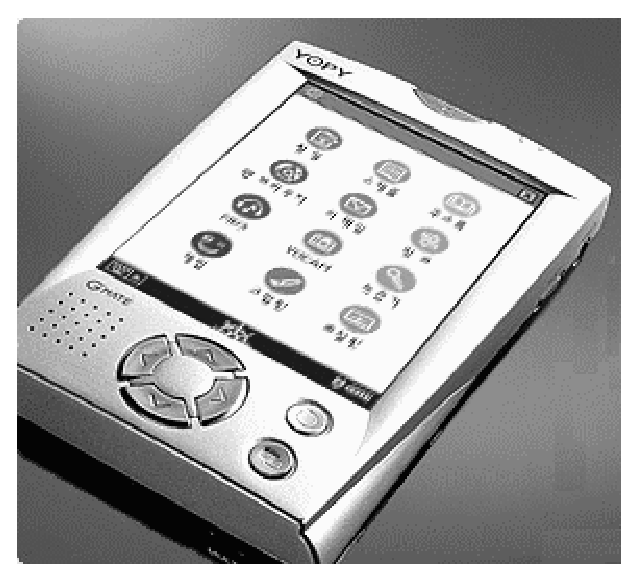
\includegraphics[width=7.0cm]{mw/bilder/yopy.eps}
    \caption{Der G.Mate Yopy}
    \label{mw_yopy}
  \end{figure}
  
  Nachdem Samsung jedoch aus dem Projekt ausgestiegen ist, ist es
  ruhig um den Yopy geworden. In Deutschland war kein solches Ger�t
  auszumachen.  Somit kam dieser PDA leider nicht f�r das Projekt in
  Frage, zumal seine Zukunft nach wie vor ungekl�rt ist und somit eine
  Versorgung der Nullserie des L�ufers mit Ger�ten nicht sicher war.
  
  Auf der Cebit 2002 wurde der Yopy wieder gezeigt, nun jedoch vom
  mechanischen Aufbau komplett anders in �hnlichkeit zu einem
  Mobiltelefon.  Diese Form pa�t nicht zu den Anforderungen an einen
  PDA im L�ufer, weshalb sich die Entscheidung gegen diesen PDA auch
  im Nachhinein als richtig erwiesen hat.

  
\item[VTech Helio] Siehe Abbildung \ref{mw_helio}.  Dies ist
  eigentlich ein PDA der Firma VTech, der mit dem propriet�ren VT-OS
  als Betriebssystem betrieben wird.  Zu diesem PDA unterst�tzt VTech
  allerdings auch die Entwicklung einer Linux-Distribution.
  \begin{figure}
    \center
    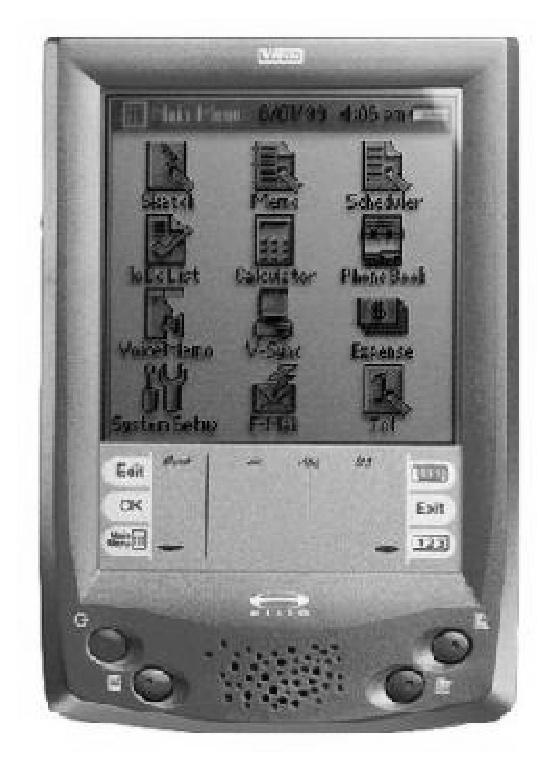
\includegraphics[width=7.0cm]{mw/bilder/helio.eps}
    \caption{Der VTech Helio}
    \label{mw_helio}
  \end{figure}
  
  Der PDA macht von seiner �u�eren Erscheinung mehr den Eindruck eines
  Spielger�tes f�r Kinder, was ja auch der Haupt-Markt des Anbieters
  VTech ist.  Der PDA verf�gt ausserdem nicht �ber ein Farb-Display,
  so da� er f�r das Projekt ebenfalls nicht in Frage kam.
  
  
\item[Casio Cassiopeia] Die PDAs dieser Serie sind �beraus
  leistungsf�hig.  Sie verf�gen �ber einen Prozessor auf Basis der
  MIPS-Architektur bei 125MHz-150MHz, bis zu 32MB RAM und Farbdisplays
  mit einer Aufl�sung von 320x240 Pixel.  Auf der Seite der Hardware
  spricht also vieles f�r den Cassiopeia. Abbildung \ref{mw_casio}
  zeigt den Cassiopeia.
  
  \begin{figure}
    \center
    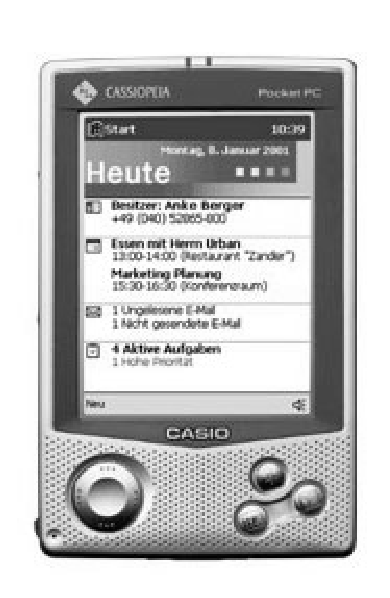
\includegraphics[width=7.0cm]{mw/bilder/casio.eps}
    \caption{Der Casio Cassiopeia}
    \label{mw_casio}
  \end{figure}
  
  Es ist auch eine Implementierung des Linux Kernels f�r diese Ger�te
  verf�gbar.  Allerdings besitzen die Ger�te dieser Serie kein
  wiederbeschreibbares Flash-ROM, sondern nur ein ROM f�r das
  Betriebssystem, so da� ein Start von Linux immer �ber spezielles
  Windows-CE Programm namens ,,CyaCE'' erfolgen mu�.  Dies ist jedoch
  im Rahmen einer \emph{Produkt}entwicklung nicht w�nschenswert, da
  sich ein potentieller Nutzer nicht zu sehr mit den technischem
  Details des Fahrzeuges auseinandersetzen m�ssen soll.
  
  Ein weiteres, nicht zu untersch�tzendes Argument gegen die Ger�te
  dieser Serie ist, da� sie von einem Asiatischen Hersteller vertrieben
  werden, und diese sich bisher als eher unwillige Sponsoren des Projektes
  erwiesen haben.

\item[Sharp Zaurus] Dieser PDA verf�gt �ber �hnliche technische Daten
  wie der Compaq IPAQ.  Wie dieser verf�gt er �ber einen StrongARM
  206MHz Prozessor, 64MB RAM und 16MB Flash.  Auch das Display ist
  �hnlich dem des Compaq. Abbildung \ref{mw_sharp} zeigt dieses Ger�t.

  \begin{figure}
    \center
    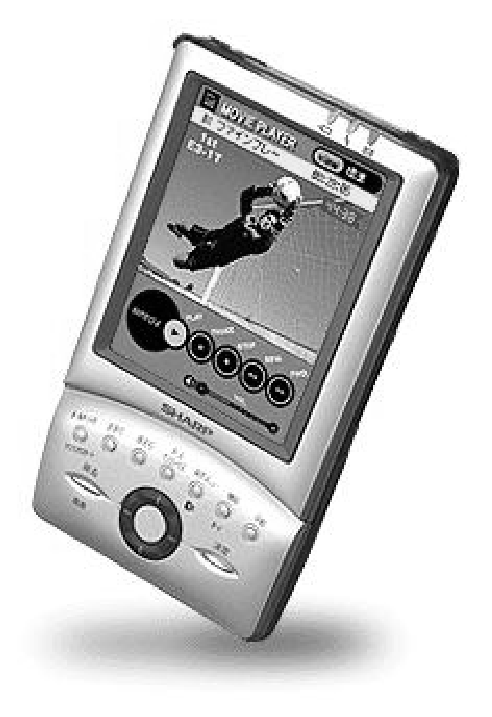
\includegraphics[width=7.0cm]{mw/bilder/sharp.eps}
    \caption{Der Sharp Zaurus}
    \label{mw_sharp}
  \end{figure}
  
  Allerdings wird dieser zu Beginn dieser Arbeit noch nicht mit einem
  Namen versehene PDA nicht mit Windows CE, sondern mit Linux als
  Betriebssystem ausgeliefert. Die Software entspricht weitgehend der,
  die wir auf dem IPAQ einsetzen. Es kommt also ein Linux Kernel 2.4.X
  mit QTopia als graphischer Oberfl�che zum Einsatz.

  Leider war das Ger�t zu Beginn unserer Arbeit noch nicht verf�gbar,
  so da� wir dieses von all seinen Daten her ideale Ger�t leider
  nicht verwenden konnten.  Auf der Cebit 2002 wurden erste Kontakte
  mit Sharp gekn�pft, um ein eventuelles Wechseln auf diesen PDA
  vorzubereiten.
  
  
\item[Compaq IPAQ] Der Compaq IPAQ (siehe auch Abbildung
  \ref{mw_ipaq_bild}ist von der Hardware her dem Sharp-PDA sehr
  �hnlich, der einzige Unterschied liegt in der standardm��ig
  ausgelieferten Software.  Der IPAQ kommt standardm��ig mit Windows
  CE, w�hrend der Sharp mit Linux ausgestattet wird.
  \begin{figure}
    \center
    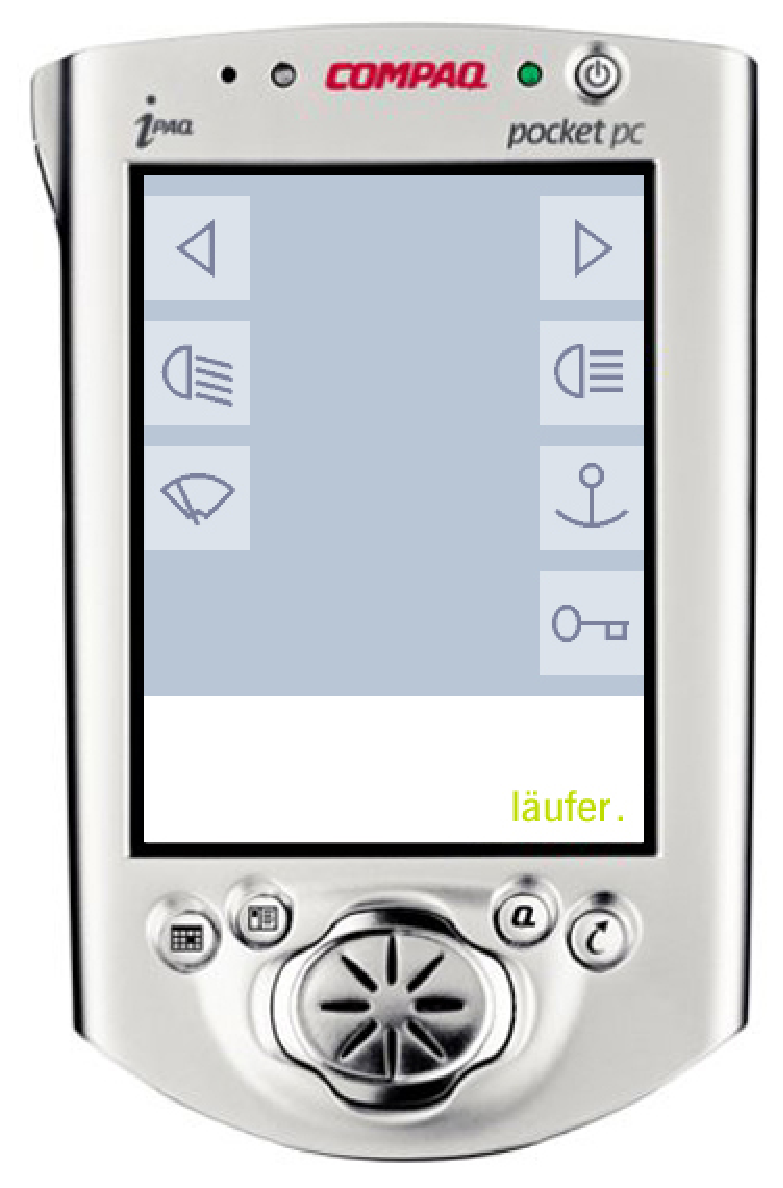
\includegraphics[width=7.0cm]{mw/bilder/Menu.eps}
    \caption{Der Compaq IPAQ mit der L�ufer-Software f�r die Cebit 2002}
    \label{mw_ipaq_bild}
  \end{figure}

  F�r den IPAQ existiert allerdings eine sehr weit fortgeschrittene
  Portierung des Linux Kernels und etlicher Programme, so da�
  mittlerweile sogar schon mehrere Distributionen um die Gunst des
  IPAQ-Besitzers buhlen.  Siehe dazu auch Kapitel \ref{mw_ipaq_linux}
  
  Die Hardware des IPAQ H3660 stellt wohl derzeit das technisch
  machbare im PDA-Umfeld dar und bietet Leistungen, die ein Entwickeln
  auf normalen Desktop-Rechnern erm�glicht, ohne das Unbehagen, die
  Zielplattform k�nnte eine bestimmte Funktionalit�t aus Gr�nden der
  dort vorhandenen Ressourcen nicht zur Verf�gung stellen.
  
  Die Hardware des IPAQ im Einzelnen:
  
  \begin{description}
  \item[CPU]
    StrongARM 206MHz
  \item[RAM]
    64MB
  \item[Flash]
    16MB interner Flash-Speicher
  \item[Display]
    240x320 12Bit reflektives Farbdisplay
  \item[Schnittstellen]
    RS-232, USB, IRDA, Analog Sound
  \item[Erweiterungen]
    
    Es besteht die M�glichkeit, den IPAQ um folgende Slots zu
    erweitern: CompactFlash, 1x PCMCIA oder 2x PCMCIA.  Hierzu wird
    der IPAQ in seine eigene Erweiterung, ein so genanntes ,,Jacket''
    hineingesteckt, was Ver�nderungen im Formfaktor zur Folge hat. Die
    Jackets gibt es in Ausf�hrungen mit den genannten
    Steckplatz-Konfiguration.
  \end{description}
  
\end{description}



\subsubsection{Entscheidung}
Die Wahl fiel letztlich auf einen Compaq IPAQ, da dieser nach den
Informationen, die zur Zeit der Entscheidung im WWW zur Verf�gung
standen, �ber die weitestgehende Unterst�tzung unter Linux verf�gt.
Ein weiteres wesentliches Argument f�r dieses Ger�t ist das reflektive
Display, wodurch eine Nutzung als zentrale Anzeige in einem Fahrzeug
�berhaupt erst m�glich wird.  Durch dieses Display wird die Anzeige
des IPAQ bei st�rkerer Sonneneinstrahlung automatisch heller, so da�
im Gegensatz zu z.B. Notebooks ein Ablesen auch im Sommer bei gro�er
Helligkeit m�glich ist.

Leider war es zu Beginn dieser Arbeit nicht m�glich, den Sharp Zaurus
zu ber�cksichtigen, da dieser zu diesem Zeitpunkt nicht zur Verf�gung
stand.  Im weiteren Projektverlauf wird allerdings versucht, auf
diesen PDA umzusteigen, da er �ber �hnliche Leistungen wie der IPAQ
verf�gt, jedoch direkt mit Linux ausgeliefert wird.  Diese Verwendung
eines Standard-PDA macht vor dem Hintergrund einer
\emph{Produkt}entwicklung nat�rlich Sinn.


\subsection{Zusammenfassung}
Wie weiter oben beschrieben wurde die Entscheidung zugunsten von Linux
gef�llt, da Linux auf dem PDA sehr PC-�hnlich zu programmieren ist und
�ber Multitasking verf�gt.  Au�erdem ist es im Bereich der GUI sehr
flexibel und es ist nicht unbedingt ein PDA n�tig, um Komponenten f�r
die L�ufer-Software zu entwickeln.

F�r den IPAQ wurde sich entschieden, weil er die beste Wahl nach dem
noch nicht verf�gbaren Sharp Zaurus darstellt.  Das Ger�t verf�gte als
erstes am Markt �ber ein \emph{reflektives}
TFT-Display\footnote{TFT=Thin Film Transistor}, was den Einsatz in
einem offenen Fahrzeug �berhaupt erst m�glich macht.  Im Laufe des
Projektes wurden im Rahmen des Cebit-Auftritts des L�ufers erste
Kontakte zu Sharp aufgebaut, um diesen PDA f�r die Nullserie gegen
einen Sharp Zaurus zu ersetzen.


\newpage
\section{Auswahl der Linux-Distribution}
\subsection{Anforderungen}
F�r den IPAQ standen zum Zeitpunkt der Entscheidung mehrere
Linux-Distributionen zur Auswahl.  Es mu�te sich also innerhalb des
Projektes f�r eine entschieden werden.  Dabei waren die Anforderungen
der Entwickler mechatronischer Komponenten ebenso zu ber�cksichtigen
wie die sp�terer Nutzer des L�ufers.

F�r Entwickler ist es am wichtigsten, da� ihnen die Entwicklung f�r
das System m�glichst leicht gemacht wird.  Dies schlie�t eine
ordentliche Programmierschnittstelle ebenso ein wie gute Werkzeuge zum
Erstellen der Graphischen Benutzerschnittstelle.  Aber auch ein gutes
Management der Softwareinstallation auf dem Ger�t ist dem Entwickler
wichtig.

F�r den Anwender ist der Mehrfachnutzen des Ger�tes entscheidend.  Es
soll zus�tzlich noch als ,,normaler'' PDA nutzbar bleiben.  Dazu
geh�rt eine ausgereifte Auswahl an Anwendungen zur Termin- und
Adre�verwaltung.  Aber nat�rlich auch ein Umfangreiches
Softwareangebot, was auch die M�glichkeit bietet, neue Versionen der
installierten Software einfach einspielen zu k�nnen.  Dies gilt
nat�rlich insbesondere f�r die Systemsoftware, also die Distribution
an sich, aber auch f�r die f�r den L�ufer speziell angefertigte
Software.



\subsection{Die Alternativen}\label{mw_ipaq_linux}
Compaq selbst unterst�tzt ma�geblich die Portierung des Linux-Kernels,
ist aber mittlerweile aus der Entwicklung einer eigenen darauf
aufsetzenden Distribution ausgestiegen, da mehrere aus der Sicht
Compaqs besser Alternativen zur Verf�gung stehen.  Zur Entstehungszeit
dieser Arbeit befindet sich Linux auf PDAs und insbesondere auf dem
IPAQ unter dem Einflu� starker Entwicklert�tigkeit, so da� viele
Distributionen und Programme sich noch im Zustand ,,Projekt'' befinden
und erst nach und nach zu ,,Produkten'' werden.  Das prominenteste
,,Produkt'' d�rfte der Sharp Zaurus sein, dessen Software weitgehend
mit der freien Oberfl�che OPIE �bereinstimmt.

Im folgenden sollen die einzelnen Projekte, die sich um Linux auf dem
IPAQ bem�hen, vorgestellt werden.  Wie auch schon bei der �bersicht
�ber aktuelle Linux-PDAs (siehe \ref{mw_pda_uebersicht}) kann und soll
hier kein vollst�ndiger �berblick �ber diese Projekte gegeben werden.
Die Projekte, die hier genannt werden, sind die, die im Rahmen dieser
Studienarbeit n�her untersucht wurden.\\
Im einzelnen sind dies:

\begin{description}
\item[PocketLinux] PocketLinux\cite{plinux} kann man wohl mit Fug und
  Recht als das ambitionierteste Projekt bezeichnen.  PocketLinux
  setzt sich aus einem Linux-Kernel, eine Java Virtual Machine sowie
  einer XML-basierten GUI zusammen.  Leider hat ein kurzer Test der
  Version f�r x86-Linux zu der Erkenntnis gef�hrt, da� die Kombination
  Java+XML+PDA wohl (noch) nicht performat genug ist, um die Anspr�che
  des Projekts L�ufer an das Ansprechverhalten der Software zu
  erf�llen.
  
  Mittlerweile wurde die Entwicklung dieses Systems auch eingestellt.
  Die Entwicklung der Java VM geht allerdings weiter und wird als
  eigenst�ndige VM f�r Embedded Devices entwickelt.

\item[Familiar Linux] Familiar\cite{flinux} ist die Brot-Und-Butter
  Distribution von Linux auf dem IPAQ.  In Ihr sind auch die fr�heren
  Compaq-Distri\-butionen aufgegangen.
  
  Familiar verf�gt �ber ein Debian-�hnliches Paketsystem, wodurch die
  Installation weiterer Software sehr einfach m�glich ist.  Jede
  verf�gbare Software ist hierzu in Pakete organisiert, die wom�glich
  untereinander durch Beziehungen verbunden sind.  Die Pakete
  werden dazu automatisch aus dem Internet geladen und eventuelle
  Abh�ngigkeiten zu anderen Softwarepaketen werden aufgel�st.  Dies
  erspart dem Anwender die von anderen Linux-Systemen bekannten
  Probleme mit Abh�ngigkeiten zwischen Softwarepaketen.  So f�hrt
  z.B. die Installation eines graphischen Programms automatisch zur
  Installation der ben�tigten Umgebung.  F�r dieses System existieren
  verschiedene Graphische Frontends, so da� die Handhabung der
  Softwareverwaltung f�r den Anwender sehr einfach m�glich ist.
  
  In der Standardinstallation verwendet Familiar das von
  UNIX-Workstations bekannte XWindow System in der Version 11 (kurz
  X11) als Graphische Schnittstelle, es existieren aber auch andere
  Graphische Oberfl�chen.  Die Portierung bestehender Anwendungen ist
  recht einfach, da X11 als Fenstersystem auf nahezu jeder auf UNIX
  oder seinen Artverwandten basierenden Workstation Verwendung findet.
  Allerdings sind diese Anwendungen in der Regel nicht auf den kleinen
  Bildschirm des PDA hin optimiert, da an UNIX Workstations historisch
  gesehen schon immer sehr gro�e Monitore mit gro�er Aufl�sung �blich
  waren.  Ebenfalls verf�gbar sind die ersten X11-basierte
  Anwendungen, die speziell f�r Familiar entwickelt wurden.  Diese
  Anwendungen decken den Bereich der Organizer-Software ab und
  ber�cksichtigen nat�rlich die spezielle Hardware, auf der sie laufen
  sollen.
  
\item[Intimate] Das Ziel dieses Projektes ist es, ein komplettes
  Debian-Linux auf den IPAQ zu bringen.  Dies ist nat�rlich nicht in
  den internen 16MB Flashspeicher als Festplattenersatz des IPAQ
  m�glich.  Deshalb setzt die Installation von Intimate zwingend das
  Vorhandensein einer externen Speicherm�glichkeit voraus.  Meistens
  ist dies wohl ein IBM Microdrive , das 1GB an Speicher im Formfaktor
  einer CompactFlash-Karte bietet.

  Intimate entsch�digt f�r diesen Aufwand mit einer Softwareauswahl,
  die (fast) auf dem Niveau von Linux auf Intel-Rechnern liegt.
  Insbesondere sind die bekannten Pakte wie Gnome, KDE, Mozilla, Emacs
  und andere verf�gbar.  Diese Anwendungen leiden jedoch unter dem
  kleinen Display des PDA, das �ber eine Aufl�sung von 240x320 Pixel
  verf�gt.  
  
  F�r den L�ufer ist allerdings diese weitgehende Verf�gbarkeit von
  Desktop- und Server-Anwendungen nicht unbedingt erforderlich, ja
  sogar hinderlich, da es im Bereich der XWindow-Anwendungen derzeit
  noch keine wirklich zufriedenstellende Software f�r den PDA-Einsatz
  gibt.  Die ben�tigte Festplatte braucht �berdies recht viel Strom,
  wodurch sich Intimate f�r die gegebene Anwendung als ungeeignet
  erwies.


\item[QTOPIA] QTOPIA ist keine eigene Distribution, sondern ein Set
  von PDA-Anwendungen die auf der QT-Bibliothek des Norwegischen
  Herstellers Trolltech basieren. 
  
  Diese Bibliothek wurde in der Version QT/Embedded (QTE) speziell an
  die Bed�rfnisse von PDAs angepa�t.  QTE ben�tigt kein XWindow
  System, sondern operiert direkt auf dem Linux Framebuffer.  Dadurch
  spart es Speicherplatz und Rechenzeit, verliert aber den Vorteil von
  X11, n�mlich die Netzwerkfunktionalit�t.
  
  QTE ist je nach Art der Kompilierung voll Sourcecode-kompatibel zu
  den anderen QT-Varianten f�r Windows, XWindow, MacOS, etc.  Um aus
  einer bestehenden QT-Anwendung f�r z.B. das XWindow System eine
  Anwendung f�r den PDA zu machen, Bedarf es keiner �nderungen,
  vorausgesetzt die GUI pa�t auf den Bildschirm des PDA.  Dies
  vereinfacht die Entwicklung ungemein.

  QT genie�t au�erdem den Ruf einer sehr guten Dokumentation, was
  den Entwicklern mechatronischer Komponenten sicher zugute kommen
  sollte.
  
  QTOPIA stellt nun eine komplette PDA-Umgebung auf Basis dieser
  Klassenbibliothek zur Verf�gung.  Dies beginnt mit den
  Rahmenbedingungen, wie verschiedenen Formen der Texteingabe
  (Handschrift, Virtuelle Tastatur, T9\footnote{Bei T9 werden wie beim
    Handy die Worte nach einigen wenigen Zeichen erkannt} etc.) und
  umfa�t auch einen ordentlichen Grundstock an Anwendungen, die man
  auf einem PDA erwartet.  Dazu geh�ren neben der
  PIM\footnote{Personal Information Manager}-Suite auch ein Betrachter
  f�r Dateien von Tabellenkalkulationen, ein Webbrowser sowie
  Email-Client und nicht zuletzt eine Anzahl an Spielen.
  
  QTOPIA findet z.B. auf dem Sharp Zaurus Verwendung, was f�r die
  Produktreife dieser Software spricht.
\end{description}

\subsection{Die Entscheidung}
F�r die Verwendung im L�ufer wurde QTOPIA auf Familiar gew�hlt, da
dies unter den gegebenen Umst�nden die fortgeschrittenste Wahl
darstellte.  Familiar mit X11 kam trotz der technischen �berlegenheit
des XWindow Systems nicht zum Zuge, da es an guten PDA Anwendungen f�r
diese Grafikschnittstelle fehlte.  QTOPIA ist explizit f�r diesen
Zweck entwickelt und stellt �ber dies sogar eine sehr gute
Programmierschnittstelle zur Verf�gung.

Auch die Aussicht auf kommerziell verf�gbare PDAs mit diesem System
beeinflu�te die Entscheidung ma�geblich, genauso wie die Qualit�t
anderer auf QT aufsetzender Softwarepakete wie z.B. KDE.



\newpage
\section{Klassenbibliothek}

\subsection{Anforderungen}
Die den Entwicklern mechatronischer Komponenten zur Verf�gung
gestellte Programmierschnittstelle bestimmt ma�geblich deren
Produktivit�t und die Qualit�t der von ihnen erstellten Software.  Aus
diesem Grund kommt dieser Klassenbibliothek eine besondere Bedeutung
zu, die in etwa der des richtigen PDAs aus der Sicht der sp�teren
Nutzer des L�ufers entspricht.

Die Programmierschnittstelle hat zwei wichtige Aufgaben: Die
Bereitstellung einer einfach zu verwendenden Kommunikation zwischen
PDA und Platinen sowie eine Schnittstellendefinition zwischen PDA
Software und dem Interface, mit dem der Fahrer auf die Fahrzeugsysteme
zugreifen kann.

Dabei m�ssen die f�r das Projekt spezifischen Randbedingungen
Beachtung finden: Zu diesen Randbedingungen z�hlt, da� mehrere
Entwickler parallel und wahrscheinlich ohne Kenntnis voneinander an
Komponenten f�r den L�ufer arbeiten werden. Au�erdem war zu Beginn
dieser Arbeit noch nicht vollst�ndig sicher, �ber welche
mechatronischen Systeme der L�ufer mal verf�gen wird.  Trotz dieses
unsicheren Umfeldes m�ssen die gesamten Software- und
Hardware-Komponenten am Ende der Entwicklung an einer Stelle zentral
zusammengef�hrt und kontrolliert werden k�nnen.

Es ist also notwendig, die Entwickler so gut es m�glich ist voneinander
unabh�ngig zu machen, es aber trotzdem zu erm�glichen, deren Arbeit am
Ende in einem Gesamtsystem zusammen zu f�hren.


\subsection{Die Kommunikation im L�ufer aus PDA Sicht}\label{mw_com}
Um die Entwickler mechatronischer Komponenten f�r den L�ufer
voneinander zu trennen, ist eine Kommunikationsstruktur notwendig, die dem
durch die Bereitstellung virtueller privater Verbindungen zwischen PDA
Software und Platine Rechnung tr�gt.  Somit wurde ein Designmerkmal
des CANBus' dieser Anforderung geopfert.  F�r die n�heren Details
dieses Aspekts verweise ich auf Kapitel \ref{jameson_kapitel}.  Hier
soll nun im folgenden auf die Anwender- bzw. Entwicklersicht auf diese
Kommunikation vom PDA aus eingegangen werden.

Grundbausteine der Kommunikation im L�ufer sind so genannte
Nachrichten\footnote{im folgenden auch: Message}, die von einem
Bus\-teil\-nehmer zum anderen gesendet werden.  Jeder Busteilnehmer
erh�lt dazu eine im System eindeutige Nummer, die sogenannte
ID\footnote{ID: f�r IDentifier}.  �ber diese Komponenten-ID wird die
Verbindung zwischen einem realen Ger�t, also z.B. einem
Scheibenwischer und dem entsprechenden Treiber auf dem PDA
hergestellt.  Die Kommunikationsstruktur des L�ufers macht dies f�r
den Entwickler transparent, d.h. er mu� sich lediglich darum k�mmern,
da� sich sein Ger�t und der dazugeh�rige Treiber unter der selben ID
beim System anmelden.

Die eigentliche Kommunikation erfolgt dann wie schon gesagt in Form
von Nachrichten, die zwischen dem Treiber und dem zu ihm geh�renden
Ger�t ausgetauscht werden.  Bei diesen Nachrichten handelt es sich
immer um einen Befehl (8Bit) mit optionalen Parametern (15Bytes).
Dadurch kann sich jeder Entwickler f�r sein Ger�t einen eigenen Satz
an Befehlen definieren, ohne da� dieser den anderen Teilnehmern im
System bekannt sein mu�.[FIXME - Referenz Jameson]



\subsection{Implementierung}\label{mw_klasse}
Ziel der Entwicklung der Klassenbibliothek ist es, die Entwicklung
darauf aufsetzender Komponenten so einfach wie m�glich zu machen, da
die Entwickler, die diese entwickeln werden, dies nur als Teil ihrer
Aufgabe auffassen k�nnen.  Die auf dieser Bibliothek aufsetzenden
Module sind genauer:

\begin{description}
\item[Treiber] Diese Komponenten stellen ein Interface zu den
  einzelnen mechatronischen Komponenten her.  Dazu sollen sie das
  Ger�t durch eine Klasse repr�sentieren, die als Methoden die
  speziellen F�higkeiten dieses Ger�tes exportiert.  Hierzu ist es
  n�tig, den Entwicklern durch diese Klassenbibliothek ein Interface
  zum CANBus zur Verf�gung zu stellen.  Au�erdem m�ssen diese Treiber
  auf Nachrichten sowohl von der GUI als auch von ihrem Ger�t am
  CANBus reagieren k�nnen.
  
\item[GUI] Die GUI soll sp�ter das Interface zum Fahrer darstellen.
  In ihr werden alle F�den zusammengef�hrt werden, die als Methoden
  aus den einzelnen Klassen laufen.  Dazu mu� es f�r den Entwickler
  dieser GUI einfach sein, auf die Methoden der Treiber zuzugreifen
  und deren Statusmeldungen zu erhalten.
\end{description}

Diese Module sind nicht Teil dieser Studienarbeit, da ihre
Implementierung im falle der Treiber am besten durch den Entwickler
der mechatronischen Komponenten durchgef�hrt wird.  Nur dieser hat das
Detailwissen, um die Treiber dem mechatronischen Ger�t angemessen zu
entwickeln.  Im Falle der GUI kann diese erst dann erstellt werden,
wenn alle Fahrzeugkomponenten feststehen, da in ihr auch die
Fahrzeuglogik festgehalten wird.  Um diese Logik zu implementieren,
bedarf es genauerer Kenntnisse der Fahrdynamik des L�ufers als die
Autoren dieser Arbeit haben k�nnen, schon aufgrund ihrer Fachrichtung.

Aufgabe ist es also, zwei Schnittstellen zu definieren. Im einzelnen
sind dies die Anbindung der GUI an die Treiber sowie die Kommunikation
zwischen Treiber und CANBus.

\subsection{Anbindung der GUI an die Treiber}
Die GUI mu� Befehle an die Treiber geben k�nnen.  Dies l��t sich
recht einfach dadurch erreichen, da� die Treiber als lokale Variablen
in der GUI Vorliegen.  Die GUI wird also zum Hauptbestandteil des
Software-Systems des L�ufers.

Die umgekehrte Kommunikation gestaltet sich etwas schwieriger.  Bei
dieser Anbindung der GUI an die Treiber kann man grunds�tzlich
Verschiedene Wege gehen:
\begin{description}
\item[Callback] Zum einen kann man allen Treibern bei der
  Initialisierung einen Pointer auf die GUI �bergeben.  Dabei mu�
  aber jeder Treiber die GUI und ihre Methoden schon kennen.  Da diese
  aber nicht Teil dieser Arbeit sein kann, ist diese verbreitete
  Methode f�r unsere Anwendung leider nicht sehr geeignet.
  
\item[Polling] Die GUI k�nnte auch die Treiber in regelm��igen
  Abst�nden Pollen, d.h. eine bestimmte im Framework zu definierende 
  Methode der Treiber-Objekte aufrufen.  �ber diesen Mechanismus w�rde
  dann jeder Treiber Rechenzeit erhalten und k�nnte eingehende
  Nachrichten bearbeiten.
  
  Diese Methode bietet die gew�nschte Flexibilit�t, da die GUI nur
  noch die Treiber kennen mu�, aber nicht umgekehrt.  Allerdings ist
  es offensichtlich, da� ein solches Vorgehen starke Probleme
  hinsichtlich der Leistung hat.  Zum einen wird so keine
  bedarfsgerechte Verteilung der CPU Leistung erreicht und zum anderen
  kostet das unn�tige Aufrufen von Methoden, die derzeit nichts zu tun
  haben, unn�tig Rechenzeit.
  
\item[Signals und Slots] Da f�r die GUI das Produkt ,,QTOPIA'' der
  Firma Trolltech zum Einsatz kommt, stand eine weitere M�glichkeit
  diese Anbindung zu realisieren zur Verf�gung.  Da dies im Gegensatz
  zu den anderen Ans�tzen nicht zu den Standard-Techniken geh�rt, soll
  hier eine Erl�uterung dieses Verfahrens gegeben werden.
  
  QT verf�gt �ber einen Mechanismus, der mit sogenannten ,,Signals''
  und ,,Slots'' arbeitet.  Signale und Slots k�nnen eine beliebige
  Anzahl Argumente beliebigen Typs �bermitteln und sind �berdies
  typsicher.
    
  Ein Objekt verschickt Signale, durch welche Slots von verkn�pften
  (connected) Objekten aufgerufen werden. Am besten l��t sich dies an
  einem kleinen Beispiel zeigen:
  
\begin{verbatim}
class Foo : public QObject
 {
  Q\_OBJECT
  public:
    Foo();
    int  value() const { return val; }
  public slots:
    void setValue( int );
  signals:
    void valueChanged( int );
  private:
    int  val;
 };
\end{verbatim}
    
  Die Ausdr�cke ,,Q\_OBJECT'', ,,slots'' und ,,signals'' werden vom
  Meta Object Compiler (moc) ben�tigt.  Dieser Compiler erzeugt ein
  neues C++-Sourcefile, das Code enth�lt, der das Objekt
  initialisiert.  Dieses File mu� compiliert und zu den anderen
  Objekt-Files gelinkt werden.  Die genannten Ausdr�cke werden vom
  Pr�prozessor entfernt bzw. so ver�ndert, da� der C++-Compiler den
  Code problemlos �bersetzen kann.
    
  Die Implementation von Foo::setValue():
\begin{verbatim}
void Foo::setValue( int v ) 
 {
   if ( v != val ) {
    val = v;
    emit valueChanged(v);
   }
 }
\end{verbatim}
  
  Ein weiterer moc-Ausdruck ist ,,emit'', womit ein Signal versendet
  wird.  Nun werden zwei Instanzen von Foo miteinander verbunden:

\begin{verbatim}
Foo a, b;
connect(&a, SIGNAL(valueChanged(int)), &b, SLOT(setValue(int)));
b.setValue( 11 );
a.setValue( 79 );
b.value();          // gibt 79 zur�ck
\end{verbatim}
    
  Durch Aufrufen von a.setValue() verschickt a ein Signal, worauf der
  damit verbundene Slot b.setValue() aufgerufen wird.
  
  Durch den Signal/Slot-Mechanismus von QT k�nnen zwei Objekte
  zusammen\-arbeiten, ohne da� sie sich gegenseitig kennen (es mu�
  nur jemand da sein, der sie verkn�pft).  Dies erleichtert die
  Programmierung von GUIs ungemein, da in einem neuen
  Widget\footnote{Element einer graphischen Oberfl�che} oft
  Standardkomponenten wie Pushbuttons etc. eingebunden werden m�ssen.
  QT �bernimmt f�r den Programmierer die Verwaltung solcher
  Standardkomponenten, sie m�ssen nur dynamisch alloziert (mit new)
  und connected werden.
  
  Genau dies ist aber auch bei der Kommunikation im L�ufer mehr als
  n�tzlich: Die Treiber k�nnen unabh�ngig von der GUI entwickelt
  werden und auch in eventuellen Nachfolgeprojekten Verwendung finden.
  Sie stellen ihre Funktionalit�t als Slot zur Verf�gung und emittieren
  Signale, wenn sie der GUI etwas mitteilen wollen.  Wohin diese
  Signale dann geleitet werden, ist Sache desjenigen, der den Treiber
  verwenden wird.
  
  Diese Flexibilit�t gab den Ausschlag f�r eine Entscheidung zugunsten
  dieser Art der Anbindung.  Informationen �ber QT finden sich unter
  \cite{mwtt}.  Der einzige Nachteil dieser L�sung ist die
  Abh�ngigkeit von QT, was bei der Nutzung von QT als GUI f�r den PDA
  aber kein gro�es Hindernis darstellt.

\end{description}

\subsection{Zugriff der Treiber auf den CANBus}
F�r den Zugriff auf den CANBus kann man ebenfalls die sehr m�chtigen
Strukturen von QTOPIA nutzen.  In diesem Fall sendet das Framework ein
Signal, da� eine neue Nachricht vorliegt.  �ber einen
Verteilermechanismus w�rde diese Nachricht dann als Signal an einen
Slot des entsprechenden Treibers gesendet.

Im L�ufer wird dieser Ansatz allerdings nicht verfolgt.  Statt dessen
erben alle Treiber von einer gemeinsamen Basisklasse, die die
Funktionalit�t des Sendens und Empfangens von Nachrichten zur
Verf�gung stellt.  Das Empfangen ist dabei eine abstrakte virtuelle
Methode, die von jedem Treiber einzeln implementiert werden mu�.  Zu
diesem Vorgehen haben zwei �berlegungen gef�hrt:

Zum einen den Teil der Bibliothek, der nicht direkt mit der GUI
zusammenh�ngt, m�glichst portabel zu gestalten.  Dies bedeutet auch,
da� man sich in diesem Bereich nicht von QT's Pr�prozessor abh�ngig
machen kann.

Zum anderen sind die anzubietenden Funktionalit�ten in diesem Bereich
wesentlich �bersichtlicher und auch schon im Laufe dieser Arbeit
bekannt: Das Senden und Empfangen von Nachrichten.  Diese genaue
Kenntnis der anzubietenden Funktionen nicht zu nutzen w�rde unn�tige
Komplexit�t im Programm hervorrufen und die Bibliothek nur unn�tig
vergr��ern.

\subsection{Implementierungsdetails}
Abbildung \ref{mw_uml} zeigt ein UML der entstandenen Bibliothek.  Auf
weitere Details zur Implementierung soll an dieser Stelle unter
Hinweis auf die im Anhang vorhandene API\footnote{API: Application
  Programming Interface}-Referenz verzichtet werden.

\begin{figure}
  \center 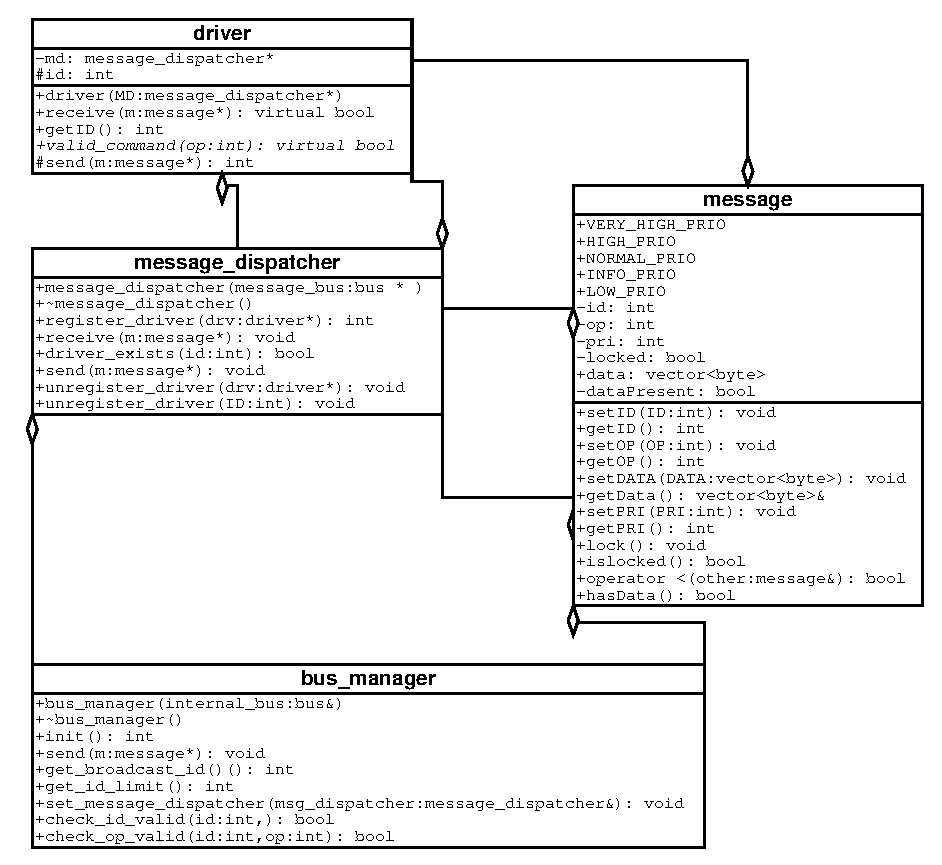
\includegraphics[width=15.0cm]{mw/bilder/uml.eps}
  \caption{UML der Klassenbibliothek}
  \label{mw_uml}
\end{figure}


%------------------------------------------------------------
\newpage
\section{Entstandene Software: DebugTreiber}

\subsection{Zweck des Tools}
Im Rahmen der Gespr�che mit den ebenfalls am Projekt L�ufer
beteiligten Maschinenbau-Studenten kam immer mehr zum Vorschein, da�
diese f�r die Entwicklung der mechatronischen Teile noch zus�tzliche
Werkzeuge ben�tigen.  So ist es f�r eine z�gige Entwicklung von
Komponenten nicht vertretbar, die Hardware parallel zum Treiber
entwickeln zu m�ssen.

Ein Entwickler z.B. eines Blinkers sollte die M�glichkeit erhalten,
seine Hardware zu testen, ohne tats�chlich schon den Treiber dazu
entwickelt zu haben. Da dieser Entwickler ja wei�, welche
ID\footnote{Diese jeder Komponente eindeutig zugeordnete Nummer mu�
  allerdings f�r jedes mechatronische Gesamtsystem zentral vergeben
  werden, da ein globaler Addressraum, wie ihn z.B. Ethernet bietet,
  nicht zur verf�gung steht.}sein Ger�t hat und welche Operationen es
versteht, kann er diese manuell eingeben und die korrekte
Funktionsweise entweder anhand von �nderungen am Ger�t selber (z.B.:
Lampe blinkt) oder aber anhand von R�ckmeldung �ber den CAN-Bus
beurteilen.  Genau dies soll der DebugTreiber erm�glichen: Manuelles
Senden und Empfangen von Nachrichten an ein bzw. von einem bestimmten
Ger�t, um den Hardware-Entwicklern die Arbeit zu erleichtern.

Da wir bei der Kommunikation zwischen Ger�t und Treiber(siehe
\ref{mw_com}) ein hinreichend generisches Verfahren einsetzen, war es
leicht m�glich, ein Programm zu entwickeln, das einen solchen
,,Handbetrieb'' eines Ger�tes erm�glicht.

\subsection{Funktionalit�ts�bersicht}

\subsubsection{Senden}
Abbildung \ref{mw_screen_senden} zeigt die GUI zum Senden einer
Message an ein Ger�t am CAN-Bus.  Wie in \ref{mw_com} beschrieben setzt
sich das Protokoll aus Operationen und eventuellen Parametern
zusammen.

Diese Messages kann man hier (numerisch) zusammenstellen, um dem unter
,,Setup'' eingestellten Ger�t eine Message zu senden.  Die GUI sollte
weitgehend selbsterkl�rend sein.  Sie verhindert, da� man zwar
Parameter eingibt, diese aber nicht gesendet werden, indem man vorher
ausw�hlen mu�, wieviele Parameter es denn werden sollen.  Dies
geschieht mit dem Eingabefeld ,,Anzahl Datenbytes''.

Dieses Tool kann (und will) allerdings nicht verhindern, da� einem
Ger�t Befehle gesendet werden, die dieses nicht verstehen kann.  Dies
mu� der Benutzer sicherstellen, der ja in der Regel mit dem Entwickler
des Treibers f�r dieses Ger�t identisch sein wird.

\begin{figure}
  \center
  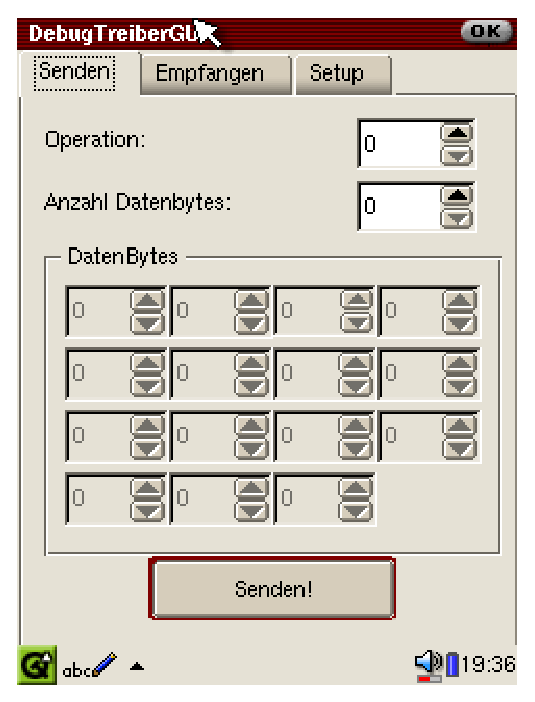
\includegraphics[width=5.0cm]{mw/bilder/GUI_senden.eps}
  \caption{Screenshot Senden}
  \label{mw_screen_senden}
\end{figure}


\subsubsection{Empfangen}
Abbildung \ref{mw_screen_empfangen} zeigt die GUI zum Empfangen von
Messages vom CAN-Bus.  Das Tool speichert eingehende Messages, die
unter der im ,,Setup'' eingestellten ID eintreffen.

Mit dem Feld ,,�bertragung'' kann man ausw�hlen, welche der
gespeicherten Messages man betrachten m�chte.  Dieses Feld zeigt
standardm��ig immer die Nummer der letzten empfangenen Message an.

Da dieser Wechsel jedoch recht h�ufig sehr schnell von statten gehen
kann, ist es m�glich, diesen Proze� zu pausieren.  Dies geschieht
mittels des Kontrollfeldes ,,Pause''.  Einkommende Nachrichten werden
bei dieser Einstellung nat�rlich weiterhin im Hintergrund archiviert.

\begin{figure}
  \center 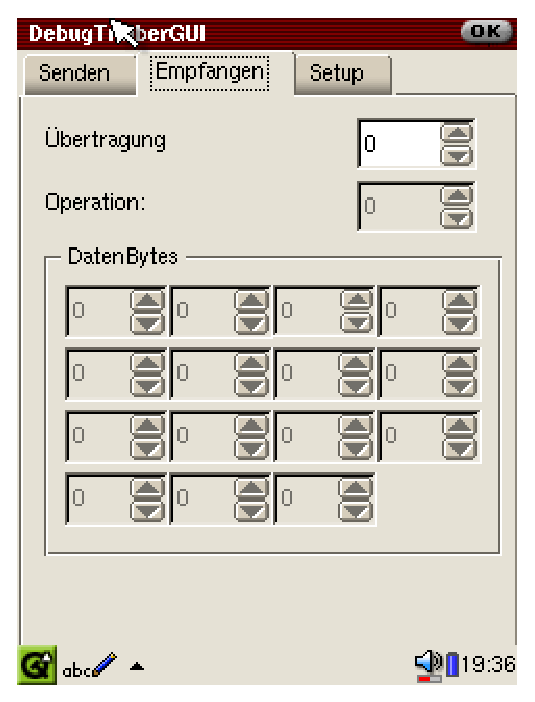
\includegraphics[width=5.0cm]{mw/bilder/GUI_empfangen.eps}
  \caption{Screenshot Empfangen}
  \label{mw_screen_empfangen}
\end{figure}

\subsubsection{Setup}
Abbildung \ref{mw_screen_setup} zeigt die GUI zum Einrichten des
Debug-Tools.  Hier kann man die gew�nschte ID des Ger�tes einstellen,
f�r das sich das Tool als Treiber registriert.  Alternativ kann man
hier ausw�hlen, einen sogenannten ,,Broadcast'' zu erstellen, der dann an
alle Busteilnehmer gesendet wird.

\begin{figure}
  \center 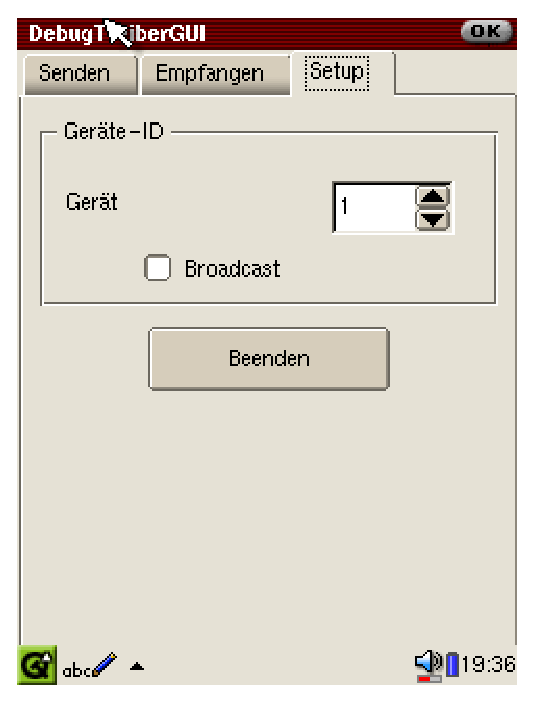
\includegraphics[width=7.0cm]{mw/bilder/GUI_setup.eps}
  \caption{Screenshot Setup}
  \label{mw_screen_setup}
\end{figure}


\newpage
\section{Fazit}
Im Rahmen dieses Teilbereichs der Mechatronik-Entwicklung f�r das
Projekt L�ufer wurde der Rahmen f�r das Fahrerinformationssystem des
L�ufers entworfen und implementiert.  Dieser Rahmen wird dann von den
Maschinenbauern mit ihrer spezifischen Fachkenntnis ausgef�llt
werden.

Da� das Framework hinreichend Leistungsf�hig ist, bewies die z�gige
Entwicklung der Demo f�r die Cebit 2002, bei der der L�ufer und seine
Mechatronik ausgestellt wurde.  Abbildung \ref{mw_cebit_gui} zeigt die
hierzu entwickelte GUI.  Auch bei dieser Entwicklung hat sich die Wahl
von Linux als PDA-System bew�hrt, da umfangreicher Support seitens der
Entwickler auf den entsprechenden Mailinglisten gegeben wurde, ohne
den eine solch schnelle Entwicklung sicher nicht m�glich gewesen w�re.

\begin{figure}
  \center 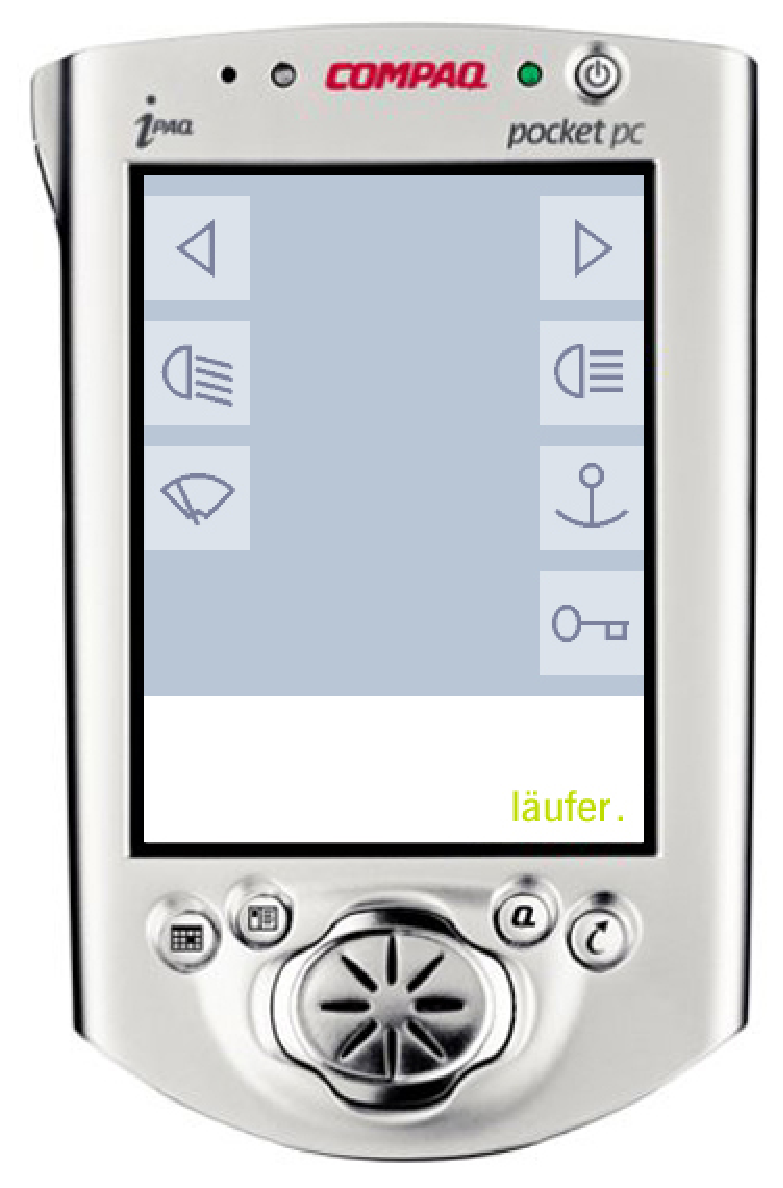
\includegraphics[width=7.0cm]{mw/bilder/Menu.eps}
  \caption{Der Compaq IPAQ mit der L�ufer-Software f�r die Cebit 2002}
  \label{mw_cebit_gui} 
\end{figure}





%%% Local Variables:
%%% mode: latex 
%%% TeX-master: "master"
%%% End:



% Jamesons Kaptitel
\chapter{Kommunikation}\label{jameson_kapitel}
von: Christoph Reichenbach
\section{Einleitung}

%--???--%
% Platine von 12V bis 48V

\section{Vor�berlegung: Zentralisiert oder F�deralistisch?}

Bevor wir uns in die faszinierende Welt der Daten�bertragung st�rzen, sollten wir, jedenfalls
f�r dieses spezielle Projekt, eine Grundsatzentscheidung treffen: Wollen wir ein m�glich
zentral gesteuertes Netzwerk verwenden, in dem das Maximum an Entscheidungen vom PDA
getroffen wird, oder diese Entscheidungen, soweit m�glich, den zu verwenden vorgesehenen SX-Platinen �berlassen?


Ein Vorteil einer zentralistisch angelegten Steuerung scheint, jedenfalls bei einem Reisefahrzeug,
nur schwer erkennbar; der �bliche Grund f�r solche Konstruktionen, die Minimierung von Redundanzen, greift
in einem Netz von konzeptionell ohnehin separaten Einheiten nicht. Somit sollten wir, um den
Daten�bertragungsaufwand zu minimieren, nur mehr Konfigurationsinformationen vom PDA an die Peripherie,
und umgekehrt nur wirklich auf dem PDA notwendige Informationen versenden; letztere lassen sich zusammenfassend
als f�r den Fahrer gedachte Angaben-- Geschwindigkeit, Akkumulatorstand-- und zur Weiterleitung an andere
Ger�te vorgesehene Informationen wie Zust�nde von als Peripherie angeschlossenen Lichtschaltern oder Blinker-Hebeln
beschreiben\footnote{Das Vorkommen der letztgenannten Informationen ist nicht zwingend erforderlich, falls
die Peripherie unmittelbar miteinander kommunizieren kann, z.B. durch eine Direktverbindung oder in einem
Multi-Master-Bussysstem.}.

\newpage

\section{Anforderungen an die Kommunikation}

Kommunikation, wenn nicht Selbstzweck-- wie bei allen Dingen-- mu� an der Me�latte
dessen beurteilt werden, was ihr Ziel und Zweck ist. Um von einer ``guten'' oder ``schlechten''
L�sung unsres Kommunikationsproblemes sprechen zu k�nnen, stellt sich uns somit zun�chst die Aufgabe,
die zur Bemessung der gesuchten Qualit�t dienenden Kriterien niederzuschreiben und auszuformulieren,
nicht zuletzt gegeneinander abzuw�gen, denn eine vollst�ndige Ordnung mu� sein, jedenfalls f�r ein
eindeutiges Urteil.

Das diese Abw�gung nicht einfach sein mu�, ist einleuchtend, doch f�hren wir sie trotz dieser
Vor�berlegung zun�chst aus, um eine Beurteilungsbasis zu bilden. Was also sind jene Me�latten,
die wir unsrer Kommunikationsl�sung anlegen wollen?

	\subsection{Korrektheit}

	Alle �bertragenen Daten m�ssen korrekt sein.


	Zu diesem Punkt mu� mehr gesagt werden, als sein Name hergibt. Korrektheit findet sich auf mehrere
	Arten und Weisen in unseren Forderungen wieder, die wir hier, milde axiomatisiert, auflisten wollen:

	\begin{enumerate}
	  \item{Wenn ein Datum den Empf�nger nicht erreicht, mu� der Sender davon erfahren}\label{j-correct-0}
	  \item{Wenn ein Datum den Empf�nger erreicht, mu� es zuvor versandt worden sein}\label{j-correct-1}
	  \item{Wenn ein Datum den Empf�nger mehrfach erreicht, mu� seine Semantik idempotent sein}\label{j-correct-2}
	\end{enumerate}

	Von diesen drei Forderungen ist insbesondere die Nummer \ref{j-correct-2} erl�uterungsbed�rftig. In Kommunikationssystemen
	kommt es erfahrungsgem�� vor, da� versandte Pakete aufgrund von unangemessen ausgel�sten Fehlerbehandlungen (�blicherweise,
	wenn die Best�tigung der Gegenseite einem unbemerkten �bertragunsfehler zum Opfer fiel) wiederholt versandt werden.
	Unsre obige Forderung ist nun auf zwei Weisen erf�llbar, n�mlich zum Einen, indem verhindert wird, da�
	der Empf�nger die Botschaft mehrfach erh�lt, oder zum Anderen, indem auf einer h�hergelegenen Interpretationsebene (auf die
	somit diese Fehlerbehandlung verschoben wird) der Doppelempfang ohne Folgen bleibt.

	Die erste Forderung ist in der Praxis auf eine sehr hohe Protokollebene verschiebbar, insbesondere, da wir Bidirektionalit�t fordern, ihr
	wesentlicher Vorteil, die Erkennung einer Situation, in der ein bestimmtes Ger�t vom Netz abgetrennt wurde, jedoch in
	genau dieser Situation f�r dessen bed�rfende Ger�te durch erzwungene Antworten auf alle an den Empf�nger gerichteten
	Anfragen erreicht werden kann.

	Diese drei Implikationen werden unsre Grundforderungen bilden. Da wir jedoch jenseits der Wunderbaren Welt der
	theoretischen Informatik operieren, werden sie nat�rlich nur ``in den allermeisten F�llen'' erf�llbar sein,
	aber diese Aussage bezieht sich nat�rlich auf alle unsre Forderungen. Diese speziellen Forderungen jedoch sind von der
	Art, in der sich wenig Verhandlungsspielraum-- im Gegensatz, zum Beispiel, zur �bertragungsgeschwindigkeit-- ergibt, somit
	m�ssen wir bei von uns gew�hlten Technologien stets auf ihre Erf�llung oder Erf�llbarkeit achten.

	\subsubsection{Bedeutung der Forderungen}

	Die Forderungen selbst sind �brigens durch ein triviales Modell bereits erf�llbar, einen {\it wissentlichen Nichtverschicker},
	der kein Datum versendet und den Sender davon in Kenntnis setzt (was die erste Forderung unmittelbar und die beiden anderen
	trivial erf�llt). Die Forderung, da� �berhaupt Daten �bertragen werden k�nnen, m�ssen wir somit auch ausdr�cken.

	%

	\subsection{Hinreichende Daten�bertragungsrate}

	Die Geschwindigkeit, mit der Daten �bertragen werden, mu� den Anforderungen des Projektes gen�gen.


	Diese Anforderung ist, in einer derartigen Formulierung, von kaum zu �bertreffender Ungenauigkeit, doch eine
	pr�zise Formulierung der ben�tigten Daten�bertragungsrate scheint in der gegebenen Situation kaum m�glich, insbesondere,
	da die Menge der anzuschlie�enden Ger�te nicht fest gegeben ist und somit nur eine Absch�tzung gemacht werden kann,
	wieviel diese dann schlie�lich an ``laufenden'' Informationen ben�tigen beziehungsweise versenden.

	Unsre Vor�berlegung jedoch, den Ger�ten gr��tm�gliche Autonomie zu gew�hren, legt nahe, da� die Bandbreite �berschaubar
	bleiben kann; betrachten wir dazu einen typischen Extremfall:

	\subsubsection{Schnelles Tachyometer}

	Typische Geschwindigkeitsmesser in verwandten Fahrzeugen werden oft nicht h�ufiger als zwei Mal pro Sekunde mit neuen
	Informationen versorgt; ein genauer aufl�sendes Tachyometer k�nnte zum Beispiel mit der Fernseh-typischen Rate von 25 Hz eine
	als st�ndig aktuell erscheinendende Qualit�t erreichen; bei 24 Bit Datenlast (8 Bit Kennziffer, 16 Bit Information)
	w�ren dies folglich, in diesem Beispiel, 600 bps f�r dieses eine Ger�t.


	Auf die n�chsth�here glatte Zahl aufgerundet (um eventuellen Unw�gsamkeiten, wie Datenverlust, zumindest in einem bescheidenen Ma�e
	vorzubeugen) w�ren dies 1024, f�r eine gesch�tzte Obergrenze von 16 Ger�ten also
	16384 bps im auf Datenlast eingeschr�nkten �bertragungsverkehr-- also Kontrolldaten ignorierend-- als theoretisches Minimum.
	Das ist, aus heutiger Sicht, nicht sehr viel, was aber, nach der Vor�berlegung, unsren Erwartungen grob entspricht.


	Bandbreite alleine reicht nat�rlich nicht unbedingt; die Erz�hlung vom mit CD-ROMs beladenen G�terzug als K�nig der Bandbreite ist
	gel�ufig genug, um an eine andere h�ufige Forderung der Daten�bertragung zu erinnern.

	%

	\subsection{Geringe Latenzzeiten}

	Die Zeit, die zwischen dem Versand und dem Eintreffen eines Datenpaketes vergeht, sollte minimal sein.


	Erneut eine eher vage Forderung, die an unsere Argumentation zur nicht-Zentralisiertheit erinnert. Wie 'minimal' die Verz�gerung sein
	sollte, ist an praktischen Beispielen wohl-- abgesehen von offensichtlichen Beschr�nkungen-- am ehesten an einer doppelten
	�bertragung zwischen einem Schalter und einer anderen Peripherie, beispielsweise einem Scheinwerfer, erkennbar; hier machen sich
	hohe Latenzzeiten zwar nicht in einer gef�hrdenden, aber doch f�r den Fahrer ersichtlichen und irritierenden Weise
	bemerkbar. Bei einer nicht direkten Verdrahtung m��te also eine �bertragung zweier Botschaften innerhalb kurzer
	Zeit versandt werden k�nnen, bei
	direkter Kommunikationsm�glichkeit zwischen Schalter und Licht verringert sich dies auf eine einzelne Botschaft.

	Eine gute Latenzzeit f�r diesen Kommunikationsschritt w�re, wie im letzten Kriterium erw�hnt, 0.04s; praktisch ausreichend
	w�re jedoch auch eine schlechtere Zeit von 0.1s, da, wie erw�hnt, zu guter Letzt doch ``nur'' wieder das Empfinden des Fahrers bedient wird.

	Gerade an diesem Beispiel sieht man nat�rlich eine zuvor schon oft implizit erw�hnte notwendige Anforderung, die als n�chstes ausgef�hrt werden soll.

	%

	\subsection{Bidirektionalit�t}

	Kommunikation zwischen Peripherie und PDA sollte in beide Richtungen m�glich sein.


	Diese Forderung ergibt sich unmittelbar aus der Notwendigkeit, Informationen, wie, zum Beispiel, die aktuelle Reisegeschwindigkeit,
	aus Peripherieger�ten auszulesen.

	%

	\subsection{Unterst�tzung f�r mehr als einen Client}

	Es sollte m�glich sein, mehr als ein Peripherieger�t mit dem PDA kommunizieren zu lassen.


	�hnlich wie beim vorherigen Punkt, der Bidirektionalit�t, ergibt sich diese Notwendigkeit aus praktischen Erw�gungen. Eine
	Ermangelung an Bidirektionalit�t oder Mehr-Client-Funktionalit�t w�re zwar allgemein durch Verwendung mehrerer paralleler
	Kommunikationssysteme ausgleichbar, eine solche Konstruktion ist aufgrund des Hardware-Mehraufwandes und der grunds�tzlich
	anderen Ansteuerung jedoch separat zu handhaben. Die angeklungene Forderung nach einem eher geringen Hardware-Aufwand l��t sich
	im �brigen noch verallgemeinern, wie wir im n�chsten Punkt sehen werden.
	%

	\subsection{Geringe Ressourcenanforderungen}

	Das verwendete Kommunikationssystem soll ``m�glichst wenig'' Hardware, Strom, und Prozessorleistung der beteiligten Kommunikationssysteme
	ben�tigen.



	Eine pr�zisere Angabe jenseits von offensichtlichen Schranken des Machbaren sind hier nicht m�glich; dies ist ein eher komparatives Kriterium.

	%

	\subsection{Praktische Realisierbarkeit mit gegebenen Mitteln}

	Das Kommunikationssystem mu� an finanziellem und technischem Aufwand realistisch implementierbar sein.


	Insbesondere ist, rein komparativ gesehen, eine Unterst�tzung seitens der Sponsoren, sowohl materiell als auch
	mit Informationen und praktischer Unterst�tzung ein relevantes und jedenfalls im Zweifelsfall den Ausschlag gebendes Kriterium.
	%


	\subsection{Die Minimalanforderungen}\label{j-min-req}

	Um nun nicht unn�tig auszuschlie�en, wollen wir unsre Minimalforderungen derart formulieren, da� der Ausgleich fehlender
	Eigenschaften auf einer h�heren Ebene prinzipiell erlaubt sein soll, endg�ltiger Ausschlu� einer Technologie w�rde also nur
	erfolgen, wenn sie das Erf�llen eines der Kriterien (in einem angemessenen Ma�) prinzipiell ausschlie�en w�rde.

	Wir fordern von gew�hlten Technologien minimal, da� sie nicht ausschlie�en, da� folgende Kriterien erf�llt werden:
	\begin{enumerate}
	  \item{\bf Korrektheit}
	  \item{{\bf Hinreichende Daten�bertragungsrate}: Mindestens 16384 bps f�r Daten alleine}
	  \item{{\bf Geringe Latenzzeit}: Maximal 0.05s pro Botschaft oder 0.1s f�r zwei Botschaften\footnote{Diese beiden Kriterien sind sehr unterschiedlich, da z.B. �ber Priorisierungsmechanismen unter Umst�nden sichergestellt werden kann, da� Botschaften, die eingingen, jedoch weiterversandt werden m�ssen, eine geringere Latenzzeit haben. Auf der anderen Seite jedoch ist es-- bei einer Latenz von konstant 0.05s-- durch zus�tzlichen Bearbeitungsaufwand m�glich, da� dennoch ein wenig mehr als 0.1s ben�tigt wird. Diese Zeit betrachten wir jedoch als unerheblich und verwenden somit 0.05s als ein einfacher zu handhabendes Kriterium.}}
	  \item{\bf Bidirektionalit�t}
	  \item{\bf Unterst�tzung f�r mindestens 16 Peripherieger�te}
	  \item{{\bf Geringe Ressourcenanforderungen}: Strombedarf auf Platine abdeckbar, eventuelle Kabel maximal handels�bliche Koaxialkabel an Dicke, 
	    sonstige Hardware sollte maximal soviel Masse haben wie der Rest der SX-Platine}
	  \item{\bf Praktische Realisierbarkeit}
	\end{enumerate}


	Mit diesen sieben Kriterien werden wir nun die verschiedenen M�glichkeiten, die sich uns zur Kommunikation bieten,
	beurteilen.

\newpage

\section{Alternativen der Kommunikationshardware}

Wir werden nun eine Reihe von Alternativen durchgehen, die uns, verbunden mit verschiedenen Vor- und Nachteilen,
Kommunikation zwischen PDA und Peripherie erlauben. Im Falle einiger dieser Technologien k�nnten die ben�tigten Anschl�sse
zwar unmittelbar auf die SX-Board aufgel�tet werden, eine Kommunikation mit dem PDA w�rde jedoch einer Zwischenstation, eines
Proxys, ben�tigen. Da auf den genannten Platinen ohnehin ein serieller Anschlu� vorhanden ist, k�nnen sie, bei
entsprechender Programmierung, unmittelbar als ein solcher dienen (sofern die verwendete Kommunikationsmethode
der Forderung nach {\bf Bidirektionalit�t} gen�gt).\\

	\subsection{Einfache Hartverdrahtung}
	
	Die einfachsten Dinge sind oft auch die besten, daher wollen wir zun�chst die Direktverbindung des PDAs mit der Peripherie �ber direkte
	Kabelverbindungen betrachten.

	Diese L�sung erf�llt zun�chst unsre Minimalanforderungen, erlaubt beliebig viele Peripherieger�te und ist an Bandbreite und Latenz nur durch
	den Systembus des SX-Controllers begrenzt. Doch schon hier stellt sich die erste Frage: Wie verbindet man die Controller direkt an ihrem
	Systembus? Ein Arbitrierungsmechanismus m��te herbei, es mu� sichergestellt werden, da� keine �bertragungen verloren
	gehen\footnote{Erste Forderung der Korrektheit}. Aber
	damit haben wir schon wesentlich mehr als eine einfache Hartverdrahtung; wenn wir jedoch unser Modell beibehalten wollen, bliebe uns nur,
	die Peripherie direkt mit den Eing�ngen der SX-Ports zu verbinden. Dies w�rde nat�rlich die Anzahl der anschlie�baren Peripherieger�te unmittelbar
	beschr�nken-- die notwendigen 16 Ger�te sollten jedoch kein prinzipielles Problem darstellen.

	Eine direkte Verbindung erzwingt jedoch einen unn�tig komplexen Kabelbaum (wenn zwei Peripherieger�te direkt
	nebeneinander liegen, ist es nicht ausreichend, sie miteinander zu verbinden-- jedes von ihnen mu� einzeln verkabelt sein). Eine derartige
	Konstruktion w�rde Masse am L�ufer kosten und w�re fehleranf�llig; dennoch verbleibt die Hartverdrahtung als eine, wenn auch nicht
	optimale, M�glichkeit. Ihr Hauptvorteil, die hohe Geschwindigkeit und geringe Latenz (die durch zwischengeschaltete Verst�rker
	jedoch geringf�gig leiden d�rfte) ist im Projektrahmen zwar interessant, aber nicht fundamental ausschlaggebend.
	
	%

	\subsection{Drahtlose Kommunikation}

	Die Zusammenfassung aller drahtlosen Kommunikationsmittel in einer einzigen Sektion legt das Urteil �ber diese nat�rlich bereits nahe,
	daher will ich es ohne Umschweife ausformulieren.

	Drahtlose Kommunikation ben�tigt mehr Leistung als hartverdrahtete Kommunikation und ist st�rungsanf�lliger; da sie kein geschlossenes
	System erlaubt (jedenfalls nicht ohne harte Kryptographie, die jenseits der Schranken der praktischen Realisierbarkeit lag), ist
	somit auch die Erf�llung der Forderungen der Korrektheit nur schwerlich vorstellbar.
	%

	\subsection{Universal Serial Bus (USB)}
	%
%% -- fixme -- %%

	\subsection{IEEE 802}
	%
%% -- fixme -- %%

	\subsection{IEEE 1394 ,,Firewire''}
	%
%% -- fixme -- %%

	\subsection{Profibus}
	%
%% -- fixme -- %%

	\subsection{InterBus}
	%
%% -- fixme -- %%

	\subsection{Actuator Sensor Interface}
	%
%% -- fixme -- %%

	\subsection{Controller Area Network (CAN)}

	Das Controller Area Network, 1986 von der Robert Bosch AG zur
	Multi-Master-Kommunikation im Auftrag von Mercedes entwickelt,
	erfreut sich heutzutage einer wachsenden Beliebtheit auch bei
	anderen KFZ-Herstellern wie BMW, Porsche, Fiat etc., wird
	jedoch auch au�erhalb der Automobilbranche genutzt.


	Das CAN-Protokoll ist ein reines Kommunikationsprotokoll
	(welches auch vielfach bereits in Hardware implementiert
	wurde), bezieht sich also nicht auf die	verwendeten
	physikalischen Transfermedien und die dar�bergelegene
	``Objektschicht'' (wie die dar�berliegenden Schichten
	gem. OSI-Modell von der CAN-Spezifikation genannt
	werden). Zur Zeit existieren zwei relevante, im gleichen Netz
	ineroperable Protokollversionen:

	\subsubsection{CAN 1.2}
	Version 1.2 des Protokolls stellt Mechanismen zur
	Bus-Arbitrierung, Erkennung und Korrektur fehlerhafter
	Daten�bertragungen und einen Standard-Adressraum von 11 Bits
	f�r angeschlossene Ger�te zur Verf�gung; aufgrund einer
	protokollbedingten Einschr�nkung ist jedoch ``nur''
	eine Adressierung von 2032 Busteilnehmern m�glich.\\
	Ein zur unmittelbaren Daten�bertragung verwendetes CAN-Frame
	(der Version 1.2) maximaler Gr��e beinhaltet 8 Bytes an Daten
	und belegt (inkl. Inter-frame space, dem Abstand zweier
	Frames) 111 Bit.\\
	Das Protokoll selbst l��t die genaue Hardware-Implementierung
	offen, g�ngig sind jedoch Raten von 1 Mb/s bei minimalem
	Verdrahtungsaufwand, was unsere Minimalanforderungen mehr als
	abdeckt.


	\subsubsection{CAN 2.0}
	Diese Protokollversion unterscheidet sich von CAN 1.2
	lediglich in der optionalen Verf�gbarkeit von
	29-Bit-Bezeichnern\footnote{Die Einf�hrung dieser Erweiterung
	begr�ndet sich historisch aus von der American Society of
	Automative Engineers (SAE) gestellten Anforderungen}.

	%

	\subsection{Vehicle Area Network (VAN)}

	Dieses Netzwerk, in direkter Konkurrenz zum CAN, wurde in Frankreich entwickelt, scheint sich jedoch keiner vergleichbaren
	Popularit�t zu erfreuen. Ebenfalls als Multi-Master-f�higes
	Protokoll entworfen, wurde es 1994 ISO-standardisiert, hat
	jedoch keine (uns relevant erscheinenden) markanten Vorteile
	gegen�ber seinem Konkurrenten.

	%

	\subsection{Konklusion}

%% -- fixme -- %%
\newpage

\section{Verbleibenden Anforderungen und Umsetzung}
	\subsection{Bereits durch CAN abgedeckte Anforderungen}
	Untersuchen wir nun die gestellten Anforderungen in Bezug auf bereits
	stattgefunden habende Abdeckung durch CAN selbst:

	\begin{enumerate}
	  \item{{\bf Korrektheit}: Wir erinnern uns an die drei geforderten Eigenschaften:
	    \begin{enumerate}
	    \item{{\it Wenn ein Datum den Empf�nger nicht erreicht, mu� der Sender davon erfahren}:
	      Diese Implikation wird von CAN nicht selbst erf�llt; ein erweiterndes Protokoll m��te
	      sie sich zur Aufgabe setzen. In unmittelbarem Zusammenhang damit ergibt sich ein praktisch
	      relevantes Problem: Kurzzeitige Leitunsst�rungen k�nnen den Verlust einzelner Botschaften zur
	      Folge haben, ohne, da� die Kommunkation unbedingt zusammengebrochen w�re. Diese Situation
	      erfordert Neuversendungen der alten Daten, wird jedoch nicht von CAN abgedeckt, da dieses
	      Protokoll keine empfangenen Sendungen quittiert.
	    }
	    \item{{\it Wenn ein Datum den Empf�nger erreicht, mu� es zuvor versandt worden sein}:
	      Wird trivial von CAN erf�llt.}
	    \item{{\it Wenn ein Datum den Empf�nger mehrfach erreicht, mu� seine Semantik idempotent sein}:
	      Die Pr�misse gilt in CAN nicht, somit mu� die Konklusion nicht erf�llt werden.}
	    \end{enumerate}
	  }
	  \item{{\bf Hinreichende Transferrate}: �bliche Implementierungen liefern 1 Mb/s; bei Wahl eines hinreichend
	    intelligenten Protokolles sollte die gew�nschte Mindest-Transferrate somit zu erreichen sein:
	    Eine solche Basis-�bertragungsrate liefert,
	    bei zwischen 111 ($1 \times 8$) und 440 ($8 \times 1$) Bits
	    f�r 8 Byte, also zwischen knapp 580000 und 145000 bps alleine f�r
	    Daten \footnote{falls keine Fehlerbehandlung n�tig ist}, weit mehr,
	    als gefordert.
	  }
	  \item{{\bf Geringe Latenzzeiten}:
	    Die Latenzen in CAN sind, wie in Bus-Systemen �blich, minimal. Bei 111 f�r schlechtest
	    m�gliche Frames liegt die Latenz unter 0.00012s, was dar�berliegenden Protokollen viel
	    Freiraum einr�umt.
	  }

	  \item{{\bf Bidirektionalit�t}:
	    CAN bietet, als Multi-Master-System, verschiedenste M�glichkeiten multidirektionaler Kommunikation.
	  }

	  \item{{\bf Unterst�tzung mehr als eines Clients}: Wie angedeutet, sieht CAN 1.2 eine Adressierung von bis zu 2032 Clients vor;
	    tats�chlich k�nnte durch sp�tere Auswahl auf den Empfangenen Daten diese Menge beliebig erweitert werden
	    (was im Rahmen dieses Projektes jedoch einer Begr�ndbarkeit entbehren w�rde).}

	  \item{{\bf Geringe Ressourcenanforderungen}: Die aufgef�hrten Bedingungen (Subesektion \ref{j-min-req}) werden von der handels�blichen Hardware
	    uneingeschr�nkt erf�llt.
	  }

	  \item{{\bf Praktische Realisierbarkeit}: Bei Verwendung dieser Technologie erhielten wir Unterst�tzung durch unsre
	    Sponsoren (von denen tats�chlich eine diesbez�gliche Empfehlung ausgesprochen worden war).
	  }
	\end{enumerate}

	\subsection{Verbleibende Anforderungen}
	Die wesentliche verbleibende Anforderung ist somit die erste Forderung der Korrektheit, die eine Notifikation
	des Senders im Falle einer fehlgeschlagenen �bertragung voraussetzt. Bevor wir uns �ber die Bedeutung dieser Forderung
	klar werden


\newpage

\section{Alternativen f�r das Kommunikationsprotokoll}

Die Wahl des Bus-Systems (f�r das wir, auf externe Empfehlung hin, CAN-Controller vom Typ
MCP2510 der Firma Microchip Technology Inc.
verwenden), war somit gefallen. Diese liefern die bereits zuvor f�r diverse Absch�tzungen verwendete �bertragungsrate
von 1 Mb/s

	\subsection{DeviceNet}
%% -- fixme: Mention it at the very least -- %%

	\subsection{CANopen}
%% -- fixme: Mention it at the very least -- %%

	\subsection{Smart Distributed System (SDS)}
%% -- fixme: Mention it at the very least -- %%


	\subsection{Eigenentwicklung}
	Zuletzt blieb nun noch die M�glichkeit einer auf die Bed�rfnisse des L�ufers zugeschnittenen Eigenl�sung. Diese
	hatte zwar zun�chst den unmittelbaren Nachteil, noch nicht entworfen worden zu sein, in Anbetracht der Nicht-
	verf�gbarkeit existierender Implementierungen der andren genannten Protokolle f�r diese Plattform jedoch andererseits
	den Vorteil, mit moderaten Entwurfsaufwand den Implementierungsaufwand den Bed�rfnissen des L�ufers entsprechend
	zu gestalten.

	\subsection{Fazit}
	Schlu�endlich fiel unsre Entscheidung schon sehr fr�h auf eine eigene Entwicklung, da der Aufwand f�r eine vollst�ndige
	Implementierung bereits existierender Protokolle (soweit ihre Spezifikationen �berhaupt �ffentlich verf�gbar waren) unseres
	Ermessens nach wesentlich h�her gewesen w�re, wohingegen die Einschr�nkung eines dieser Protokolle keine
	merklichen Vorteile gegen�ber einem solchen eignen Protokoll erwirkt h�tte. 


\newpage

\section{Das L�ufer-Protokoll f�r den CAN-Bus} 

Die Aufgaben des resultierenden Protokolls lassen sich nun wieder auf die bereits zuvor verwendeten Protokollkriterien zur�ckf�hren.
Hierbei mu� jedoch darauf geachtet werden, die Eigenheiten des CAN-Protokolls zu beachten; die Protokolle haben also nicht nur zur
Aufgabe, unsere Korrektheitsforderungen zu erf�llen, sondern auch, eine gute Anbindung an CAN zu bieten-- wobei es sich von diesem
nat�rlich aus Gr�nden eines klaren Designs zumindest in seiner Spezifikation hinreichend weit abtrennen sollte.\\

Unsere Entscheidung fiel zugunsten eines zweischichtigen Protokolldesigns, in dem eines der Protokolle die grunds�tzliche Kommunikation und das
andere einfaches Session-Management mit Timeouts spezifizierte. Die Trennung dieser beiden Dinge schien uns in Hinsicht auf die
bevorstehende Implementierung, aber auch aus Sicht der Modularit�t
sinnvoll.\\

Eine zun�chst noch offene Frage war jedoch die Form der Protokolle,
gerade auch, da CAN Unterst�tzung f�r Multi-Mastering bietet. Wir
entschlossen uns zun�chst dazu, das Session-Protokoll f�r eine
Master-Slave-Kommunikation auszulegen, da dies der angestrebten unmittelbaren
Kontrolle der Peripherie durch ein zentrales System entsprach; dies
erweiterten wir sp�ter um einen Notifikationsmechanismus in die andere
Richtung und bauten es somit zu einem zwei-Master-Netz aus.
Das Netzwerk-Protokoll hingegen, das auch die Aufgabe der
Adressierung bestimmter Clients �bernehmen sollte, bildete ein
Multi-Master-System mit prioritisierten Botschaften (speziell unter Ausnutzung
der Eigenschaften des CAN-Busses), aus den gleichen Gr�nden.\\

Aus theoretischer Sicht ist das Netz somit von sternf�rmiger
Topologie, die tats�chliche Verdrahtung hingegen kann nat�rlich
beliebig im Rahmen des von CAN Erm�glichten erfolgen.

	\subsection{Die beiden Protokollschichten}
	Die beiden Protokolle, mit Namen {\it LLO} und {\it LLZ} (``L�ufer Layer One'' bzw. ``Zero''), nehmen also
	zueinander signifikant andere Aufgaben wahr:

		\subsubsection{Aufgaben des LLO-Protokolls}
		Die Aufgaben des LLO-Protokolls umfassen die folgenden:
		\begin{enumerate}
		  \item{Adressierung der Klienten}
		  \item{Verpackung der zu �bertragenden Daten in Pakete des Data Link/Network Layer (speziell CAN)}
		  \item{Busmastering}
		\end{enumerate}


		\subsubsection{Aufgaben des LLZ-Protokolls}
		Das LLZ-Protokoll �bernimmt folgende Teilaufgaben:
		\begin{enumerate}
		  \item{Session-Management}
		  \item{Erf�llung des ersten Korrektheitskriteriums}
		\end{enumerate}
		Eine ``Sitzung'' im f�r uns relevanten Sinn erstreckt sich hierbei von Aktivierung bis Deaktivierung
		des L�ufers.

		\subsubsection{Der sichere Betriebszustand}
		Beiden Protokollen ist ein Konzept zu Eigen, das den Namen ``sicherer Betriebszustand'' tr�gt, sich
		auf Klienten im Bus bezieht und
		individuell f�r jedes angeschlossene Ger�t definiert werden mu�. Dieser sichere Betriebszustand
		ist von angeschlossenen Ger�ten im Fehlerfall einzunehmen, insbesondere, wenn die Kommunikation nach
		au�en abrei�t.
\newpage

\section{Der Bezug zum OSI-Schichtenmodell}
Als kurzer Einschub soll hier noch einmal auf das OSI-Schichtenmodell
eingegangen werden, das zwar keinen leitenden Einflu� auf das Protokolldesign
hatte, wohl aber zur nachtr�glichen Klassifizierung verwendet werden kann.\\
In dem verwendeten Kommunikationssystem werden die Ebenen wie folgt belegt:

\begin{itemize}
  \item {{\bf Schicht 1: Physical Layer}: Diese Schicht findet sich in Verdrahtung, dem MCP2510, dem SX-Microcontroller, und den
    dazwischenliegenden Verbindungen.}
  \item {{\bf Schicht 2: Data Link Layer}: Die Fehlererkennung dieser Schicht ist im CAN-Protokoll spezifiziert, findet sich ent-
    sprechend physikalisch auf dem MCP2510.}
  \item {{\bf Schicht 3: Network Layer}: Ansteuerung der Komponenten wird, im Rahmen der CAN-spezifizierten Vorgaben, von einem
    von einer Implementierung des LLO-Protokolls realisiert. Die wesentliche Arbeit dabei wird durch Filtermechanismen im MCP2510
    realisiert.}
  \item {{\bf Schicht 4: Transport Layer}: Die Zerteilung in einzelne Pakete f�hrt die LLO-Implementierung durch.}
  \item {{\bf Schicht 5: Session Layer}: Die Registrierung von Busteilnehmern und Timeout-Checks bei der Kommunikation werden
    von LLZ realisiert.}
  \item {{\bf Schicht 6: Presentation Layer}: Nach- bzw. Vorbearbeitung der �bersandten Daten wird von Ger�ten und Treibern
    individuell gel�st und ist nicht Teil der hier beschriebenen Kommunikationsschicht.}
  \item {{\bf Schicht 7: Application Layer}: Die tats�chliche Durchreichung der Informationen an den Anwender, ihre optische
    Aufbereitung, automatische Beantwortung oder, allgemeiner, Versendung, findet sich in den anderen Teilen dieser Ausarbeitung
    beschrieben.}
\end{itemize}
    

\newpage

\section{Das LLO-Protokoll}\footnote{Die vollst�ndige Protokollspezifikation findet sich als Anhang (Sektion {\ref llo-proto}).}


	\subsection{Struktur des Protokolls}
	\subsection{Umsetzung}
	\subsection{Tests}

\newpage

\section{Das LLZ-Protokoll}\footnote{Die vollst�ndige Protokollspezifikation findet sich als Anhang (Sektion {\ref llz-proto}).}
	\subsection{Struktur des Protokolls}
	\subsection{Umsetzung}
	\subsection{Tests}

\newpage

\section{Fazit}


\newpage



\section{Protokoll-Layer 1: LLO-Protokoll, Version 0}
Das L�ufer Layer 1- Protokoll hat die Aufgabe, eine zielgerichtete,
sichere �bertragung von potentiell beliebigen Datenmengen in einem
Broadcast-Netzwerk mit bis zu 30 Kommunikationsteilnehmern und potentiell
begrenzter Paketgr��e durchzuf�hren. Sicher in diesem Zusammenhang bedeutet,
da� es �berpr�ft, ob ein Rezipient die f�r ihn gedachte Botschaft erhalten
hat, und, falls nicht, eine vern�nftige Anzahl von Neu�bertragungen versucht,
nach denen es den Rezipienten als vom Netz abgetrennt registriert.
Das vorliegende Netz ist dabei sternf�rmig aufgebaut.
\\
Die hier befindliche Spezifikation bezieht sich auf Version 0 des
L�ufer Layer One (LLO)-Protokolls.\\


\subsection{Kommunikation}
Das Protokoll sieht ein Multi-Master-Netzwerk als Basis vor, mit einem
Master in der Funktion des LLO-Controllers. Das Netzwerk mu� entweder
drei Klassen von Nachrichten-Priorit�ten, oder voll-Duplex-Kom-\\munikation
unterst�tzen.\\
Im Kontrast zum LLO-Controller (kurz: Controller) werden die anderen
Busteilnehmer als LLO-Clients (kurz: Clients) bezeichnet, auch, wenn diese
Bezeichnung ihre M�glichkeiten nicht voll w�rdigt.\\

In dieser Spezifikation wird Bezug auf Timeouts genommen. Diese Timeouts
werden nicht explizit spezifiziert, mit Ausnahme des Keep-Alive-Timeouts,
um Implementierern die Wahl Bus-spezifische angemessene Timeouts zu erlauben.\\


\subsubsection{Clients}
Jedem Client ist eine eindeutige Identifikationsnummer (Port) zugeordnet, die
im Addre�bereich des Protokolls liegt (0-31 in dieser Version) und nicht
0 oder 1 ist (1 ist f�r den Controller reserviert).\\
Eine Menge von Hardware ist ein Client genau dann, wenn sie sich an einem
Port P != 0 als Client im Sinne der Protokollspezifikation verh�lt.
Aus dieser Definition folgt, da� mehr als ein physikalischer Empf�nger als
Client agieren kann; die Protokollimplementierungen auf den Clients haben
in diesem Fall Vorkehrungen daf�r zu treffen, da� ihr Verhalten auch im
Fehlerfall dieser Spezifikation entspricht.\\

Jedem physikalichen Element eines Clients ist ein sicherer Betriebszustand
zugeordnet. Sobald dieses Element feststellt, da� es von den �bertragungen
des Netzes abgetrennt wurde, mu� es s�mtliche Kommunikation beenden und
den sicheren Betriebszustand einnehmen.\\
Ein Verlassen des sicheren Betriebszustandes ist nur durch Zur�cksetzen
des Ger�tes auf einer untergeordneten Ebene m�glich (z.B. Hardware-Reset).\\


\subsubsection{Controller zu Client-\"Ubertragungen}
%---------------------------------------

\paragraph{Synchrone \"Ubertragungen\\}
%------------------------------
Eine �bertragung von einem Controller zu einem Client erfolgt unangek�ndigt
mit einer Sequenz von STX-Paketen (Synchronous Transfer); aus Sicht des
Masters:

\begin{tabular}{cl}
  $\leftarrow$  & {\tt STX(id, more) size: data}\\
  $\rightarrow$	& {\tt ACK(id, more)}\\
\end{tabular}

Graphisch dargestellt:

\vspace{0.3cm}
\begin{tabular}{|c|c|c|c|}
\hline
\hline
{\tt 010IIIII } & {\tt X00MSSSS } & {\tt LLLLLLLL} & \hspace{1cm} $\cdots$ {\tt SIZE} bytes $\cdots$ \hspace{1cm} \\
\hline
\hline
\end{tabular}

\vspace{0.3cm}

\begin{tabular}{|c|c|}
\hline
\hline
	  {\tt 011IIIII }
	  &
	  {\tt X00MSSSS } \\
\hline
\hline
\end{tabular}

\vspace{0.3cm}

Wobei die Bedeutungen wie folgt sind:\vspace{0.3cm}\\

\begin{tabular}{lcp{8cm}}
{\bf Name}	& {\bf K\"urzel} & {\bf Bedeutung}\\
\hline

{\tt STX}	& {\tt 010}	& Synchronous Transfer: Operationscode\\
{\tt ACK}	& {\tt 011}	& Acknowledgement: Operationscode\\
{\tt more}	& {\tt M}	& Flag, welches indiziert, ob noch mehr Daten in diesem	Kommunikationsstrom folgen\\
{\tt size}	& {\tt L}	& Menge an folgenden Datenbytes\\
{\tt id}	& {\tt I}	& Identit\"at des Clients (Client-Kanals)\\
{\tt seqnr}	& {\tt S}	& Sequenznummer (s. \ref{j:p1:ferr})\\
{\tt reserviert}	& {\tt X}	& Reserviertes Bit\\
{\tt data}	& 	& Sequenz von {\it size} Bytes an Daten\\
\end{tabular}
\vspace{0.3cm}\\

Wenn bei einer �bertragung das {\it more}-Flag gesetzt ist, m�ssen die
Daten der n�chstes �bertragung ans Ende der vorherigen �bertragung
angeh�ngt werden.\\
Zwischen Controller und Client findet maximal eine �bertragung
gleichzeitig statt; somit ist gew�hrleistet, da� Pakete einer �bertragung
eindeutig zugeordnet werden k�nnen.\\

Ein Ausbleiben des Acknowledgements f�r eine bestimmte, imple-\\mentierungs-
abh�ngige Zeit wird als Timeout gewertet; der Sender f�hrt in diesem Fall
eine Neu�bertragung durch.\\
Nach einer angemessenen Anzahl von versuchten Neu�bertragungen wird
schliesslich eine Fehlermeldung an die aussendende Stelle ausgegeben oder
(falls keine solche Stelle existiert) intern behandelt werden.\\

\paragraph{Broadcast-�bertragung\\}
%----------------------------

Broadcast-�bertratungen entsprechen �bertragungen, bei denen die
Zieladdresse gleich 0 ist.



\subsubsection{Client zu Controller- �betragungen}
%---------------------------------------
Diese �bertragungen sind synchron und werden mit der {\tt RTX}-Operation durch-
gef�hrt:


\begin{tabular}{cl}
$\rightarrow$ & {\tt RTX(id, more) size:data}\\
$\leftarrow$  & {\tt ACK(id, more)}\\
\end {tabular}

Die �betragungen finden statt, sobald der Controller explizit mit einer
NOP-Anweisung den Bus freigibt oder pausiert. In diesem Fall werden R-�bertragungen von
dem ausgewiesenen Sender akzeptiert, bis eine �bertragung nicht mehr das
'more'-Flag gesetzt hat oder ein unbehebbarer Fehler auftrat.
Jede erfolgreiche �bertragung wird mit einem {\tt ACK} best�tigt.


\subsubsection{Fehlererkennung und -behandlung}\label{j:p1:ferr}
%-----------------------------------
Das LLO-Protokoll geht von einem selbst fehlererkennenden Protokoll aus,
daher testet es nur auf Fehler, die eine Netz-Trennung zwischen Controller
und Client indizieren.


\paragraph{Sequenznummern\\}
Jede synchrone und asynchrone �bertragung erh�ht einen Sequenzz�hler
sowohl auf der Seite des Clients wie auch des Controllers; dieser Z�hler
hat den initialen Zustand 0 und z�hlt aufw�rts, in Schritten der Gr�sse
1, Modulo 16. Sein Zustand wird in jeder �bertragung mitgesandt und danach
erh�ht, mit der expliziten Ausnahme von {\tt SYS}-,
{\tt KAL}- und {\tt NOP}-�bertragung (bei denen er nur
mitgesandt, aber nicht erh�ht wird) sowie Broadcasts\footnote{Da die Sequenznummern von
Broadcasts nicht definierbar sind. Der Nichterfolg eines Broadcasts kann somit
nur durch Timeout der Best\"atigung erkannt werden. Dies bedeutet, dass die Empfangsreihenfolge
f\"ur Broadcasts nicht garantiert ist und reduziert deren Nutzen auf globale Fehlermeldungen.}.\\
F�r {\tt STX} und {\tt RTX} werden hierbei zwei getrennte Z�hler verwendet, um
bei gepipelinetem Versandt eine eindeutige Zuordnungsf�higkeit der Nummern
zu gew�hrleisten.


\paragraph{�bertragungen im Fehlerfall\\}
Falls bei einer �bertragung ein Fehlerfall diagnostiziert wird, wird diese
�bertragung entweder entweder erneut durchgef�hrt (wenn der Fehler vom
Sender diagnostiziert wurde), oder es wird- entweder anstelle eines {\tt ACK}
(synchron) oder statt zu schweigen (asynchron) ein {\tt SYS} zur�ckgesandt:

\begin{tabular}{cl}
  $\rightarrow$ & {\tt RTX(id, more) seq=10, size:data}\\
  $\leftarrow$  & {\tt ACK(id, more) seq=11}\\
  $\rightarrow$ & {\tt RTX(id, more) seq=14, size:data}  {\bf /* FEHLER */} \\
  $\leftarrow$  & {\tt SYS(id, more) seq=12, INVSQ}      {\bf /* Fehlersignalisierung */} \\
\end{tabular}

In diesem Fall antwortet der Sender entweder ebenfalls mit {\tt SYS} (Abbruch der
�bertragung), oder er wiederholt die �bertragung an der vom erhaltenen
{\tt SYS} indizierten Stelle. Ein Abbruch erfolgt genau dann, wenn sich die
angezeigte Sequenznummer des Empf�ngers auf eine vorhergehende Botschaft
bezieht, oder wenn die Differenz der Sequenznummern modulo 16 gr�sser
oder gleich 8 ist. Der Empf�nger synchronisiert im Abbruchsfall seine
Sequenznummer mit der des Senders.
Dieser Fehlerfall kann unter folgenden Bedingungen auftreten (unter Voraus-
setzung der Korrektheit des Controllers):
a) Ein Client verwendet eine inkorrekte Protokollimplementierung
b) Ein Client hat mehrere asynchrone Pakete verpa�t
c) Ein Client besteht aus mehreren physisch Einheiten, von denen eine echte
nichtleere Teilmenge einen Teil der �bertragungen verpa�t hat.

F�r den Fall (a) kann die Korrektheit des Empfangs im Allgemeinen nicht
gew�hrleistet werden. Fall (b) ist durch Definition der inh�renten Un-
sicherheit asynchroner Pakete abgedeckt. Kritisch ist somit Fall (c):
Die empfangenden physikalischen Einheiten m�ssen erkennen, da� eine
Geschwistereinheit einen Fehler erkannt hat, und sich ruhig verhalten.
Im Falle eines �bertragungsabbruches m�ssen auch die Einheiten, die
die Nachricht korrekt erhalten haben, die aktuelle �bertragung abbrechen,
um Konsistenz zu gew�hrleisten.

\paragraph{SYN-Request\\}
%-----------------
Ein {\tt SYN}-Request ist eine synchrone {\tt STX}-�bertragung, die eine size von 0
hat. Sie dient der Synchronisierung der Sequenznummern und ist wie eine
normale �bertragung zu behandeln, soweit das Protokoll betroffen ist.

Nach sp�testens 14 asynchronen Paketen (Broadcasts) in Folge mu� ein Sender
ein {\tt SYN}-Paket schicken, um die Synchronit�t der Sequenzz�hler zu
gew�hrleisten.


\paragraph{Systemcodes\\}
%-----------------
Bei einem SYS werden Systemcodes (meist Fehlercodes) mitversandt.
Sie sind definiert wie folgt:

\begin{tabular}{ccp{4.5cm}p{4.5cm}}
{\bf NR}& {\bf ID}	& {\bf Bedeutung}				& {\bf Kommunikation}\\
\hline
1	& {\tt EINTN}	& Interner Fehler			&Abbruch\\
2	& {\tt EINSQ}	& Unpassende Sequenznummer		&Retry oder {\tt ABORT}\\
3	& {\tt ABORT}	& �bertragung Ung�ltig, Abbruch		&Abbruch\\
4	& {\tt CONTN}	& �bertragung ab hier fortgesetzt	&Fortsetzung\\
5	& {\tt EOVFL}	& Nachricht zu lang: Buffer-�berlauf	&Abbruch\\
6	& {\tt EINVR}	& Ung�ltige Version			&Abbruch\\
7	& {\tt EGLBL}	& Globales Versagen			&Sicherer Betriebszustand\\
8	& {\tt ENRDY}	& Ger�t nicht bereit			&Retry nach Verz�gerung\\
\end{tabular}
\vspace{0.3cm}

Ein SYS:GLOBL kann als Broadcast vom Controller eingesetzt werden, um alle
Ger�te in den sicheren Betriebszustand zur�ckzufahren (und damit den Bus
effektiv zu deaktivieren).


\paragraph{Timeout\\}
%-------------
Bei synchronen Versendungen wird ggf. in einem spezifizierten Zeitraum kein {\tt ACK}
vom Empf�nger erhalten. In diesem Fall wird das Paket erneut versandt


\subsection{Keep-Alive}
%-------------

Mindestens einmal pro 100 ms mu� der Controller f�r ein Keep-Alive-Signal
({\tt KAL}) auf dem Bus sorgen. Bleibt dieses Signal f�r mehr als 300 ms aus,
so m�ssen sich alle Clients in einen sicheren Betriebszustand zur�ckfahren.


\subsection{Kodierung der �bertragungspakete}
%------------------------------------
Dieses Kapitel dokumentiert die Standardkodierung der Pakete; implementierende
Systeme k�nnen eine eigene, angemessenere Kodierung verwenden.


Graphisch pr\"asentiert sich die Kodierung wie folgt:

\vspace{0.3cm}
\begin{tabular}{|c|c|c|c|}
\hline
\hline
{\tt OOOIIIII } & {\tt XVVMSSSS } & {\tt LLLLLLLL} & \hspace{1.5cm} $\cdots$ {\tt SIZE} bytes $\cdots$ \hspace{1.5cm} \\
\hline
\hline
\end{tabular}\\
\vspace{0.3cm}


{wobei manche Befehle nur zwei Bytes verwenden und die Bedeutung der Abk\"urzungen wie folgt ist:}


\begin{tabular}{cp{10cm}}
{\bf K\"urzel} & {\bf Bedeutung}\\
\hline

{\tt O}	& Synchronous Transfer: Operationscode\\
{\tt I}	& Identit\"at des Clients (Client-Kanals)\\
{\tt X}	& Reserviertes Bit\\
{\tt V}	& Versionsnummer\\
{\tt M}	& Flag, welches indiziert, ob noch mehr Daten in diesem	Kommunikationsstrom folgen\\
{\tt S}	& Sequenznummer (s. \ref{j:p1:ferr})\\
{\tt L}	& Menge an folgenden Datenbytes\\
\end{tabular}


\subsubsection{Erstes Pr�fixbyte}
%----------------------
Das erste Byte des Paketes (Pr�fixbyte) setzt sich zusammen wie folgt:\vspace{0.3cm}\\

\begin{tabular}{ll}
{\bf Bits}	& {\bf Bedeutung} \\
\hline
7-5		& Operation \\
4-0		& Rezipient \\
\end{tabular}
\vspace{0.3cm}\\


\subsubsection{Operationen}
%------------------
\vspace{0.3cm}

\begin{tabular}{ll}
{\bf Nummer}	& {\bf ID} \\
\hline
0	& {\tt NOP}\\
1	& {\tt STX}\\
2	& {\tt RTX}\\
3	& {\tt ACK}\\
4	& {\tt SYS}\\
5	& {\tt KAL}\\
\end{tabular}


\subsubsection{Zweites Pr�fixbyte}
%-----------------------
\vspace{0.3cm}

\begin{tabular}{cl}
{\bf Bits} & {\bf Bedeutung}\\
\hline
7	& Reserviert\\
6,5	& Version (hier immer 0)\\
4	& Das 'mehr'-Flag\\
3-0	& Sequenznummer\\
\end{tabular}\vspace{0.3cm}\\


\subsubsection{STX, RTX: �betragungspakete}
%--------------------------------
In diesen Paketen folgt ein Byte mit der Anzahl der zu �bertragenden
Daten-bytes, gefolgt von entsprechend vielen Daten.


\subsubsection{ACK, NOP und KAL}
%--------------------
Diese Pakete sind nach den Pr�fixbytes leer.


\subsubsection{SYS}
%-------
Auf dieses Paket folgt genau ein Byte mit dem Identifikator der System-
Message.


\subsection{Appendix A: Implementierung auf dem CAN-Bus}
%-------------------------------------------
Bei einer Implementierung auf dem CAN-Bus (LLO/CAN) wird das komplette
erste Pr�fixbyte im Identifyer dargestellt:
\ \vspace{0.1cm}\\
\begin{tabular}{cl}
{\bf Bits}	& {\bf Bedeutung}\\
\hline
10-8	& LLO/CAN-Operation\\
7-5	& Priorit�t f�r {\tt RTX}-Botschaften, sonst 011\\
4-0	& ID des Rezipienten
\end{tabular}
\ \vspace{0.1cm}\\

\subsubsection{A.1 Codierung der LLO/CAN-Operationen}
%-------------------------------------

\begin{tabular}{cccl}
{\bf Bit 10} 	& {\bf Bit 9}	& {\bf Bit 8}	& {\bf ID}\\
\hline
0	& 0	& 0	& {\tt SYS}\\
0	& 0	& 1	& {\tt ACK}\\
0	& 1	& 0	& {\tt KAL}\\
1	& 0	& 0	& {\tt STX}\\
1	& 1	& 0	& {\tt RTX}\\
1	& 1	& 1	& {\tt NOP}\\
\end{tabular}\vspace{0.3cm}\\

Somit gilt: \{{\tt SYS}, {\tt ACK}, {\tt KAL}\} $>$ \{{\tt STX}\} $>$ \{{\tt RTX}\} $>$ \{{\tt NOP}\},
wobei A $>$ B bedeutet, da� alle Elemente von A eine h�here
Priorit�t als ein beliebiges Element aus B haben.

Bei STX und RTX wird die L�ngenangabe im daf�r von
CAN vorgesehenen Bereich gespeichert, nicht als zus�tzliches
Byte. Das Protokoll verwendet im optionalen Datenbereich also
genau ein Byte.

\label{llo-proto}

\newpage


\section{Protokoll-Layer 0: LLZ-Protokoll, Version 0}
%-------------------------------------------
Alle folgenden Aussagen beziehen sich auf Version 0 des Protokolls, mit
Ausnahme explizit gekennzeichneter Stellen.\\

Das LLZ (L�ufer Layer Zero)- Protokoll realisiert eine asynchrone
und synchrone Kommunikation �ber einen existierenden sicheren Transferkanal.
'Sicher' hat hierbei die Bedeutung, da� die erfolgreiche �bertragung
mit hoher Sicherheit ``garantiert'' wird; kommt die �bertragung nicht zustande,
tritt der Garantiefall ein und es mu� ein Fehler auf
der darunterliegenden Protokollebene ausgel�st werden.
Das Protokoll unterscheidet zwischen Empf�nger- und Senderstationen, die
verschiedene Rechte und Pflichten haben.\\
Zudem ist das Protokoll Zustandsbehaftet.\\

Im folgenden bezeichnet $\prec X$ das Ereignis, da� die Botschaft X empfangen
wurde, und $X \succ$ das vollst�ndige und erfolgreiche Versenden der Botschaft X,
ebenso wie $\rightarrow X$ (Senden) und $\leftarrow X$ (Empfangen).\\

\subsection{Kommunikation}
%----------------
Jegliche Kommunikation, mit Ausnahme einer Notifikation, wird von einem
Sender ausgel�st.\\

\subsubsection{Synchrone Kommunikation}
%---------------------------

\paragraph{Operationen und Semantik\\}
F\"ur jedes Ger\"at ist eine Menge von Operationen definiert. Diese
Operationen d\"urfen durch eine bestimmte Anzahl von Bytes parameterisiert sein.
F\"ur jede mit $\overline{x}$ parametrisierte Operation $p(\overline{x})$ gilt,
da\ss\ die Semantik des Empfangs von $p{\overline{x}^\prime}$ nach $p{\overline{x}}$
gleich der Semantik des Empfangs von $p{\overline{x}^\prime}$ ist, also, da\ss\ alle
Operationen nur Zustand {\it setzen} und {\it keine relativen Modifikationen} an ihm
durchf\"uhren.
 

\paragraph{Request\\}
%-------------
Eine synchrone Kommunikation beginnt mit einem Request, der vom Sender
ausgel�st wird. Die Notation hierf�r ist (aus Sender-Sicht)\\

\begin{tabular}{cl}
$\rightarrow$ {\tt REQ(n) <OP> [Parameter]*}\\
\end{tabular}

z.B.

\begin{tabular}{cl}
$\rightarrow$ {\tt REQ(2) SET-STATE 7}\\
\end{tabular}

(n ist 1 plus die Anzahl der Parameter). Die Operation ist ein 7-Bit-Wert
(das MSB ist reserviert); die Anzahl der Parameter ist beschr�nkt auf 15.
Auf einen Request mu� ein Response folgen. Protokollimplementierungen
m�ssen also eventuell vorher eingehende Notifikationen zur�ckstellen.\\

\paragraph{Response\\}
%--------------
Aus Sender-Sicht ist die Notation hierf�r wie folgt:

\begin{tabular}{cl}
$\leftarrow$ & {\tt RES(n) <OP> [Value]*}\\
\end{tabular}

Wobei {\tt <OP>} eine Wiederholung des Operationscodes aus dem Request ist.

\paragraph{Kommando\\}
%--------------
Statt einem Request kann auch ein Kommando ({\tt CMD} statt {\tt REQ}) abgesetzt werden.
Der einzige Unterschied ist, da� keine Response hierauf generiert wird.


\subsubsection{Asynchrone Notifikation}
%---------------------------
Der Empf�nger kann asynchron Notifikationen absetzen. Diese Notifikationen
sind wie Responses aufgebaut, haben als Transmissionsoperation (s. 1.3) jedoch
{\tt NTF} statt {\tt RES}. Insbesondere beinhalten sie auch eine Operation.
Notifikationen d�rfen nur bei au�ergew�nlichen Situationen verwendet werden.
Es bleibt Senderimplementierungen vorbehalten, Empf�nger, die Notifikationen
unangemessen mi�brauchen, per {\tt SDN} zu deaktivieren.

Jeder Einheit ist jedoch eine Notifikation pro Sekunde zuzugestehen.


\subsubsection{Spezifikation der Transmissionspakete}
%-----------------------------------------
Alle �bertragungen sind Byte-basiert. Ein Transmissionspaket mit einem
Payload der L�nge n+1 sieht aus wie folgt:

\begin{tabular}{|c|c|c|c|c|}
	prfx & dat0 & dat1 & . . .  & datn\\
\end{tabular}

I.e. ein 8-Bit-Pr�fix, gefolgt von n+1 Datenbytes.

Der Pr�fix hat folgende Form:
\vspace{0.3cm}\\
\begin{tabular}{cp{1.0 cm}p{10 cm}}
{\bf Bit}	& {\bf ID}	& {\bf Bedeutung}\\
\hline
7-5	& {\tt TOP}	& Transmissionsoperation (siehe \ref{j-app-1.3.1})\\
4	& --	& reserviert (mu� 0 sein)\\
3-0	& {\tt LEN/ ERC/ VNR}
		& {\tt LEN}: Anzahl der folgenden Bytes an Daten minus 1.
		  Falls {\tt TOP} den Wert {\tt ERR} hat, ist dies der Error-
		  code; es folgen keine weiteren Daten.
		  Falls {\tt TOP} den Wert {\tt INI} oder {\tt IOK} hat, ist hier
		  die Versionsnummer des Protokolls codiert.\\
\end{tabular}


\subsubsection{Transmissionsoperationen}\label{j-app-1.3.1}
%------------------------------
\ \vspace{0.3cm}\\

\begin{tabular}{clp{10cm}}
{\bf Code}	& {\bf ID}	& {\bf Semantik}\\
\hline
0	& {\tt SDN}	& Der Empf�nger soll einen sicheren Betriebs-
		Zustand einnehmen und s�mtliche Kommunikation
		unterbinden (siehe Sektion \ref{j-app-3})\\

1	& {\tt IOK}	& Initialisierungsantwort (Protokollversion in VNR)\\

2	& {\tt REQ}	& Sender-Operation: Synchrone Anfrage\\

3	& {\tt RES}	& Empf�nger-Operation: Synchrone Antwort\\

4	& {\tt CMD}	& Sender-Operation: Asynchrones Kommando\\

5	& {\tt NTF}	& Empf�nger-Operation: Asynchrone Notifikation\\

6	& {\tt INI}	& Initialisierungsoperation, siehe Sektion \ref{j-app-3}\\

7	& {\tt ERR}	& Protokollfehler, siehe \ref{j-app-1.3.2}\\
\end{tabular}


\paragraph{Protokollfehler\\}\label{j-app-1.3.2}
%---------------------
Falls ein Sender eine ung�ltige �bertragung absetzt, mu� der Empf�nger
ihn dar�ber benachrichtigen. Zu diesem Zweck ist {\tt TOP ERR} definiert. 

Die folgenden Werte f�r {\tt ERC} sind definiert:
\ \vspace{0.3cm}\\

\begin{tabular}{lp{11cm}}
{\bf \tt ERC}	& {\bf Bedeutung} \\
\hline
0	& Sonstiger Fehler (catch-all-code) \\
1	& Version nicht unterst�tzt \\
2	& Falsche Rolle: Sender versuchte, {\tt RES}, {\tt NTF} oder {\tt IOK} zu senden \\
3	& Schon initialisiert: {\tt INI} gesendet, obwohl der Empf�nger bereits initialisiert ist \\
4	& Fehler verschickt: Der Sender sandte ein {\tt ERR} zum Empf�nger \\
5	& Paket korrupt: Ein reserviertes Bit ist falsch gesetzt \\
6-15	& -- {\it reserviert} --\\
\end{tabular}
\ \vspace{0.3cm}\\

\subsection{Payload}
%----------
LLZ v0 �bertr�gt Datenpakete einer Gr��e von 1 bis 16 Bytes. Das erste
Byte, als ``Operation'' bezeichnet, mu� immer vorhanden sein. 


\subsection{Lebenslauf von Kommunikationsteilnehmern}\label{j-app-3}
%-------------------------------------------

Der Lebenslauf von Sendern wird in dieser Spezifikation nicht behandelt.
Empf�nger jedoch werden von Sendern initialisiert und, bei Bedarf, deaktiviert;
die entsprechenden Zust�nde und �berg�nge finden sich in 3.1.


\subsubsection{Empf�nger}
%--------------
Das LLZ-Protokoll definiert folgende Zust�nde eines Empf�ngers:
\ \vspace{0.3cm}\\

\begin{tabular}{ccp{8cm}}
{\bf Code}	& {\bf Name}		& {\bf Erkl�rung}\\
\hline
{\bf S0}	& {\tt PRE-INIT}	& Initialer Zustand. Ger�t darf keine Fehlercodes senden.\\
{\bf S1}	& {\tt INIT}		& Ger�t hat INI erhalten, noch nicht beantwortet\\
{\bf S2}	& {\tt RUNNING}		& Ger�t hat IOK geantwortet und ist im normalen	Betriebszustand\\
{\bf S3}	& {\tt DOWN}		& Ger�t hat SDN erhalten und den sicheren
                                          Betriebszustand eingenommen, es darf keine Fehlercodes mehr senden. \\
\end{tabular}
\ \vspace{0.3cm}\\


%Das Zustands�bergangsdiagramm ist wie folgt:
%
%		<SDN
%	+---------------------------+
%	|			    |
%	|   <INI     IOK>     <SDN  V
%	S0 -$\rightarrow$ S1 -$\rightarrow$ S2 -$\rightarrow$ S3
%        ^	 |
%	|	 |ERR>
%	+--------+


In Zusatenden {\bf S0}, {\bf S1} und {\bf S3} werden alle Messages ignoriert, die nicht
zu einem Zustands�bergang f�hren.


\subsubsection{Shutdown}
%------------
Beim Erreichen des {\tt DOWN}-Zustandes sollte das Kommunikationsprotokoll, soweit
m�glich, das zugrundeliegende System informieren, so da� dies einen
gesicherten "Failsafe"-Betriebszustand einnehmen kann.


\subsubsection{Initialisierung des Empf�ngers}
%-----------------------------------
Die korrekte Sequenz zur Initialisierung eines Empf�ngers verl�uft aus
Sicht des SENDERS wie folgt:

\begin{tabular}{cl}
$\leftarrow$	&{\tt INI(VNR=0)}\\
$\rightarrow$	&{\tt IOK(VNR=0) ops[16]}\\
\end{tabular}

Folgt keine Antwort, so mu� der Sender annehmen, da� der Empf�nger nicht
existiert.

Statt IOK kann auch {\tt ERR(1)} (Version nicht Unterst�tzt) gesendet werden,
siehe \ref{j-app-3.3.1}.

Das Datenfeld ops[16] beinhaltet eine Liste aller vom Ger�t unterst�tzten
Operationen, codiert in 128 Bits. Der Test auf Vorhandensein der Operation
x (f�r x $>$ 7) ist also in Hochsprachensemantik wie folgt:
\ \vspace{0.2cm}\\
{\tt have-op(x) := ((x >> 3) < n) {\bf /* Byte is defined */}\\
\mbox{\hspace{2cm}\&\& (ops[x >> 3] \& (1 << (x \& 7)))}}
\ \vspace{0.2cm}\\
Dies erlaubt die Deklaration der Operationen 0-127. Die Deklaration dient
Debugzwecken und ist in dieser Protokollversion nicht verbindlich.

\paragraph{Versionsunterschiede\\}\label{j-app-3.3.1}
%--------------------------
Falls die Protokollversion des Senders vom Empf�nger nicht unterst�tzt
wird, mu� er mit {\tt ERR(1)} antworten. Der
Sender kann dann andere Protokollversionen durchprobieren, oder mit {\tt SDN} das System deaktivieren.
\label{llz-proto}

% Christians Kapitel
\chapter{Implementierung der Embedded Platinen}\label{cr_kapitel}
von: Christian R�diger
\section{Anforderungen an die Peripherieelektronik}
\subsection{Gesamtkonzept}
Die Mechatronik im Projekt L"aufer mu� einer Reihe projektspezifischer Anforderungen standhalten. Was bedeuten also die eingangs geschilderten
Zielsetzungen f�r die Peripherieelektronik?

Da sich der genaue Funktionsumfang aller mechatronischen Komponenten f"ur die Zukunft nicht absch�tzen l"asst, und neue Komponenten jederzeit einfach
einzugliedern sein sollen muss das System leicht erweiterbar sein. F�r die  Zielgruppe zur Nutzung der Platinen sind die Peripherieger�te des L"aufers
muss das System mit vertretbarem Aufwandt bedienbar sein. F�r den nutzenden Ingeneur muss der Effekt und nicht der Weg interessant sein.
Die begrenzten Resourcen eines autnomen Systems wie dem L"aufer erfordern au�erdem eine sparsame Nutzung von Energie.
Um die Fahrer nicht durch Fehlfunktionen oder Ausfall eines Ger�tes zu gef�hrden mu� das System betriebssicher sein. D.h. sowohl in der physikalischen
Auslegung als auch in der Implementierung m"ussen m"ogliche Extreme in der Nutzung des Fahrzeugs ber"ucksichtigt werden. Dies beinhaltet auch eine
gewisse Fehlertoleranz mittels ,,fail save Design''.
Nicht zuletzt muss die L�sung zum einen durch das vorhandene Know How im Umfeld des Projekt L"aufer umsetzbar als auch finanzierbar bzw. durch
Sponsoren erh�ltlich sein.
Bei der Zusammenstellung der Platine muss ausserdem auf Verf"ugbarkeit der Bauelemente sichergestellt sein.
Zu guter letzt muss eine Platine wenig Raum einnehmen um dem Design des Fahrzeugs gr"o�tm"oglichen freiraum zu gew"ahren.

Zusammengefasst ist das Ziel der Arbeit eine im mechatronischen Bereich vielseitig und einfach bedienbare Platine zu erstellen sowie die
Implementierung einer Grundfunktionalit�t.
Im folgenden wird die Umsetzung der Anforderungen im Detail besprochen.

\subsection{Flexibilit"at}
Der CAN-Bus macht ein einfaches Einklinken in den Bus an jeder erdenklichen Stelle m�glich. Dadurch ist das Gesamzkonzept schnell erweiterbar.
Ein neueres Ger�t erh�lt eien eindeutige Identifikationsnummer und wird dann durch den PDA erkannt und gesteuert. N�heres dazu findet sich im Protokollteil wieder.
Die Platine erm�glicht das Anschlie�en unterschiedlicher Ger�te ohne sich um Protokollfragen k�mmern zu m�ssen.
Die Wahl der Microcontrollers und der elektronischen Bausteine lassen dem Entwickler gr��tm�gliche Freiheit bei der Wahl der Funktionalit�t des
Peripherieger�tes. Das Layout der Platine erlaubt bei entsprechender Dimensionierung der Widerst�nde und Kondensatoren eine Versorgungsspannung von
5 bis 48 Volt. Ein Spannungswandler regelt dann die Spannung auf die f�r MOS-technologie �blichen 5 Volt herunter um die Bauelemente entsprechend zu
versorgen
\subsection{Kosten}
Die Platine enth�lt lediglich Standardbauelemente wie sie auch in der Automobilindustrie verwendet werden. Die Kosten einer komplett best�ckten Platine
belaufen sich auf etwa 150,- \geneuronarrow{}. das Layout erlaubt jedoch eine Teilbest�ckung die sich auf die f�r ein spezifisches Peripherieger�t notwendigen
Bauelemente beschr�nkt. Ein weitere wichtger Punkt bei der Kostenbestimmung war die Verwendbarkeit und das Zusammenspiel der Bauelemente in der
gew�nschten Zusammenstellung. Um gravierende Fehler auszuschlie�en und alle Vorstellungen umzusetzen begleitete die Firma Cetron den gesammten Prozess der
Platinenentwicklung. Von der Idee, dem Prototypen, der Auswahl der Komponenten, des Microcontrollers, dem Layout der Platine in zwei Revisionen bis 
hin zur Suche nach Sponsoren f�r 12 4-Layer Platinen sowie bei der Best�ckung derselben stand die Firma Cetron mit Rat und Tat bei.

Die genauen Kosten der Platine h�ngt nicht unwesentlich von der Wahl der Komponentendistributoren ab. Preisunterschiede von bis zu 400 \% (z.B. bei
blauen LEDs) sind keine
Seltenheit. Eine sorgf�ltiger Preisvergleich der m�glichen Lieferanten ist wichtiger Bestandteil der Kostenbestimmung.
\subsection{Sicherheit}
Zum Schutz vor Strom und Spannungsspitzen sowie weitestgehend vor falscher Bedienung durch einen Entwickler wurde bei der Auswahl der Komponenten als
auch beim Layout auf Robustheit Wert gelegt. Die Platine sowie die Bauelemente enthalten eine Reihe von Schutzmechanismen wie Zener-dioden oder eine
,,Schmelzsicherung'' in Form einer besonders d�nnen Leiterbahn.
Der zweite wichtige Sicherheitsaspekt liegt in der Funktion eines etwaigen Ger�tes. Hierzu sind die Nutzer der Platine angehalten einen fail save
Zustand zu implementieren. Eine entsprechende Nachricht auf Protokollseite existiert bereits.
\subsection{Design}
Um sich in das Design des L�ufers zu integrieren sind sowohl die Erweiterbarkeit als auch die simple Gr�sse der Platine von Wichtigkeit.
Die Erweiterbarkeit ist bereits im Bereich Flexibilit�t beschrieben. Die Gr��e der Platine betr�gt ca. 4,5cm * 8,6 cm, hat also etwa die Gr�sse einer Checkkarte.

\begin{figure}
  \center
  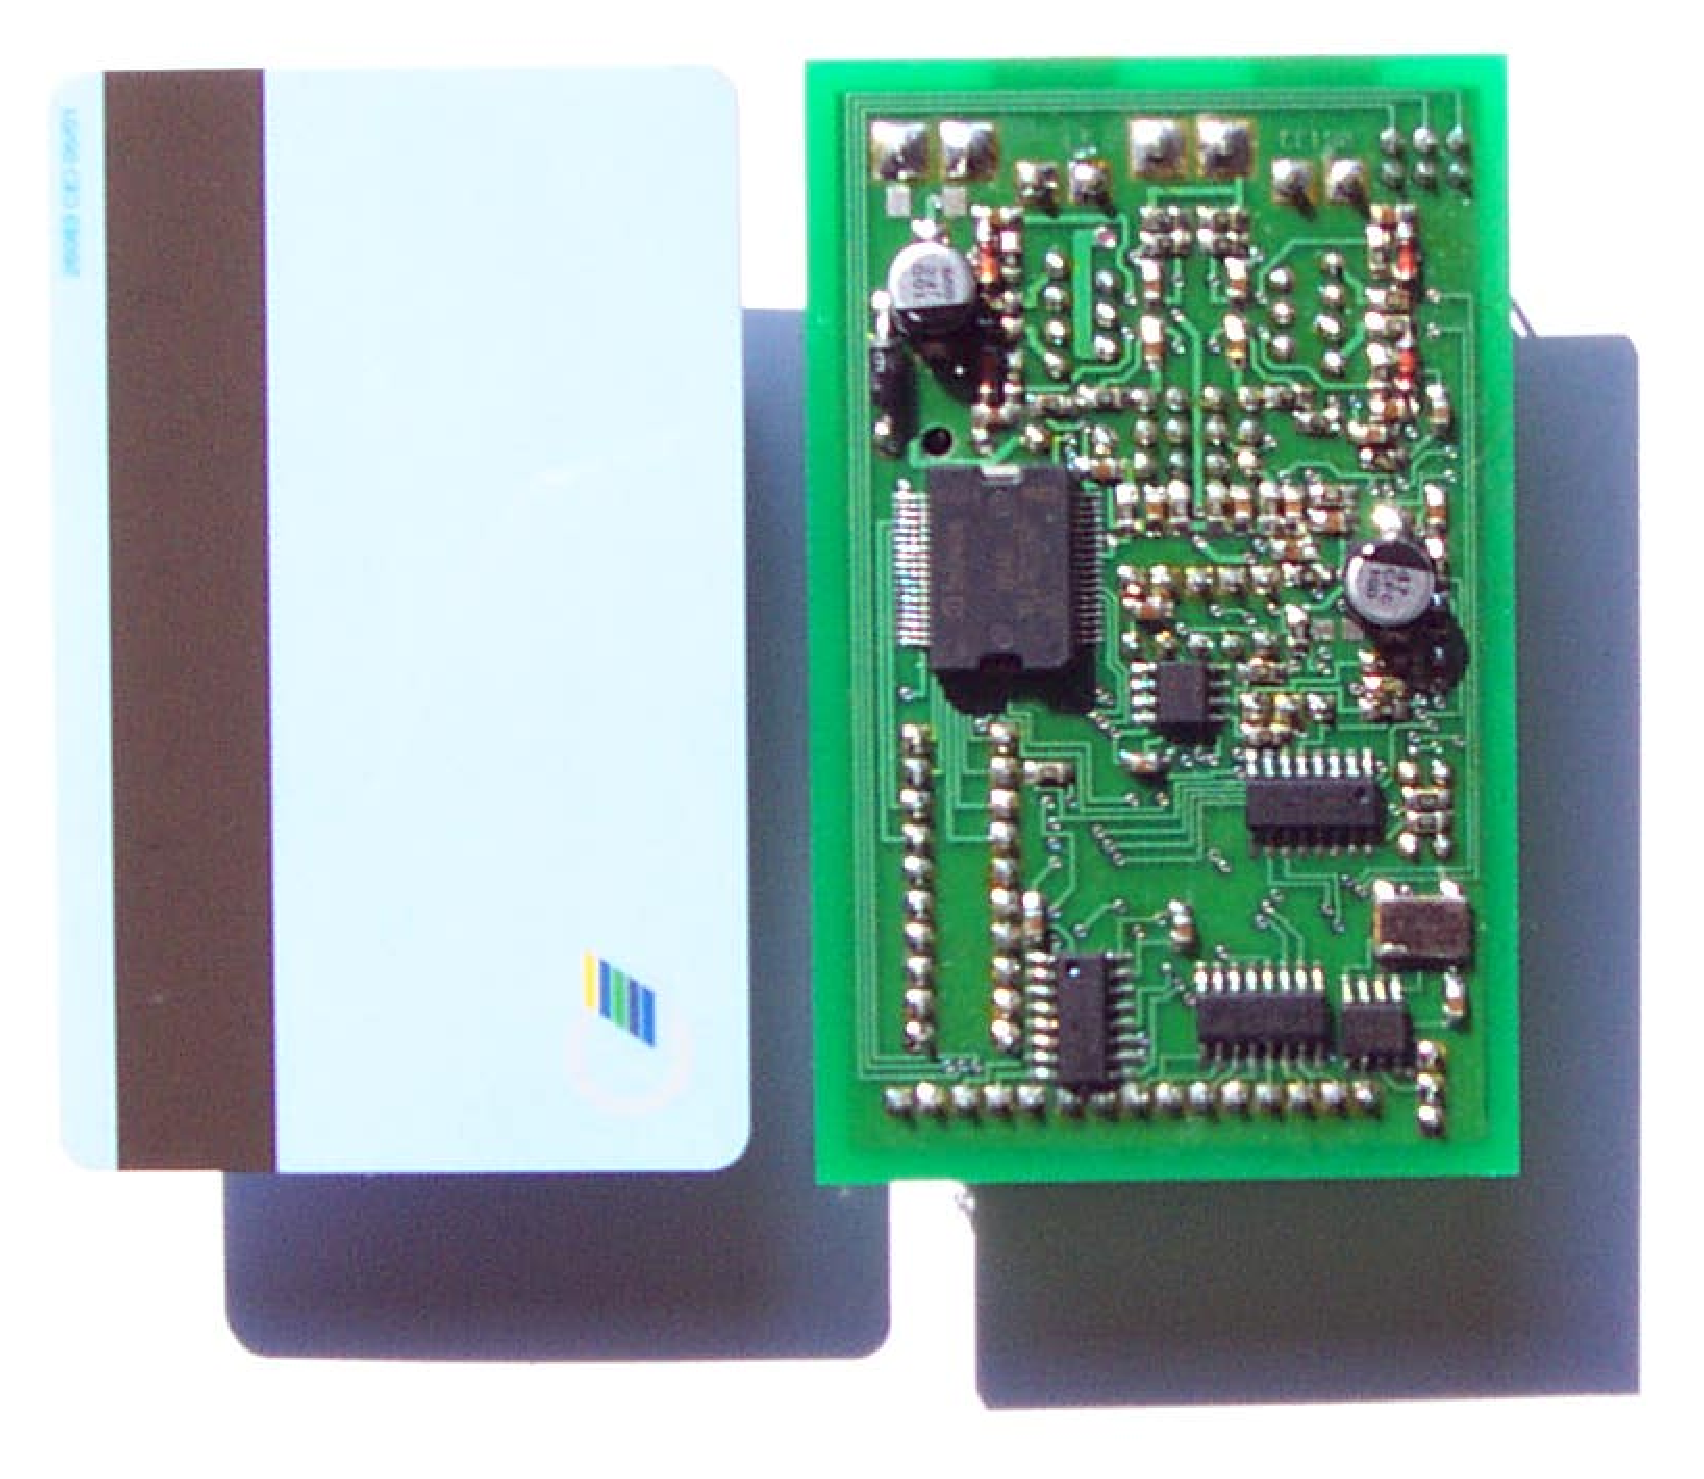
\includegraphics[width=277pt]{Platine_C-Karte.eps}
  \caption{Gr�ssenvergleich Platine Cheque Karte}
  \label{Platine-Karte}
\end{figure}


\newpage
\section{Wahl der Komponenten}
\subsection{Microcontroller}
HC-Familie Motorola

8051-Familie 
-Infineon
SAB80C35
---------------------------------------
Intels 8-Bit Industriestandard:
Vom 8008 zu 8080 und 8085, Vergleich mit Zilog Z80 22.4.2002 

Preiswert und leistungsfa"hig:
Motorola 6800 und 6809 im Vergleich zu MOS 6502 

Die 16Bit-A"ra
Die Konkurrenten:
Intel 8086/88 vs. Motorola 68K 29.4.2002

Texas Instruments TI9900, Zilog Z8000 und National Semi. NS16016

Von 16 auf 32Bit:
Intel 80286-486 und Pentium(I) vs. Motorola 68020-060 und NS16032 
-------------------------------------------------

SAB80C166

SAB C167LM

80C31

68HC11

HC12-Familie Motorola

MC68HC812A4

8-16-32 bit MCs

PIC by Microchip


Taktfrequenz
Preis
Erh�ltlich
Entwicklungsumgebung


Die Wahl des Microcontrollers beruht auf der Empfehlung der Firma Cetron. Im folgenden werden im groben die Eigenschaften beschrieben. Weitere Details
stehen im Teil \ref{Konzeption} Konzeption der Implementierung.

Die Wahl des Microcontrollers fiel auf den SX52. Dieser Microcontroller der Firma Ubicom hat 16 Seiten Programmspeicher a 512 12-Bit Worten f�r den 
Programmcode und 16 $\times$ 16 8-Bit Registerb�nke sowie eine Spezialbank zur Konfiguration. Das hei�t es stehen 8 Kilobyte (1 Byte = 12 Bit) f�r
Programmcode und $2^{8}$ 8-Bit Register zu Laufzeit zur Verf�gung. F�r Unterprogrammaufrufe steht ein Stapel mit einer Tiefe von acht Eintr�gen zur
verf�gung. Der Programmspeicher entspricht physikalisch einem Flashrom, soda� das zum Beispiel weiterentwickelte Versionen auch im nachhinein
eingespielt werden k�nnen. Diese M�glichkeit erleichtert auch die Entwicklung insofern als das Programme nicht erst in simulierter Umgebung getestet
werden muss, sondern sofort im Einsatzumfeld erprobt werden kann ohne gro�e Kosten zu verursachen.

Der SX52 hat f�nf 8-Bit Ports die sowohl als Input als auch als Output nutzbar sind. Es existiert ein Stromsparmodus (Sleep-mode) der zur Laufzeit an- und ausschltbar
ist. Der Microcontroller hat eine Interrupt-funktion die ebenfalls zur Laufzeit aktivier und deaktivierbar ist. Einer der f�nf Ports kann als
Interrupt oder Weck-port konfiguriert werden. Das hei�t ein Signal an diesem Port l�st einen Interrupt aus bzw. ,,weckt'' den Mocrocontroller aus dem
Stromsparmodus. 

Ein Besonderheit des SX ist ein komerziell erh�ltliches Programmierpaket, mithilfe dessen ein Programm schrittweise ausgef�hrt und sowohl auf
Bildschirm als auch am Microcontroller verfolgbar ist. N�hers dazu im Kapitel \ref{Umgebung} Programierumgebung.
Dies macht die Programmierarbeit deutlich einfacher.

Die Assemblersprache die der mitgelieferte Interpreter akzeptiert ist PIC-kompatiebel, so das im Internet L�sungen zu h�ufigen Problemen auzufinden
sind.

Mit einer Taktfrequenz von 50 MHz ist der SX auch f�r eine 115 Baud �bertragung an der seriellen Schnittstelle schnell genug.
Weitere f�r die Programmierung relevante Merkmale werden im Kapitel \ref{Implementierung} Implementierung besprochen.
\subsection{Peripherie}
Um eine flexible Nutzung der Platine zu sichern gilt es eine Vielzahl von Anschlu�m�glichkeiten zur Verf�gung zu stellen. Im folgenden werden die
genutzen Bauelemente und Funktionalit�ten der Platine beschrieben.
\begin{description}
\item[Serial Peripheral Interface (SPI)]
Die gro�e Anzahl an Bauelementen macht eine sparsame Nutzung der I/O-Ports am Microprozessor n�tig.
Zu diesem Zweck sind der CAN-Bus-Chip, zwei Low-Side-Switches, ein Analog-Digital-Wandler und ein Digital-Analog-Wandler �ber ein SPI-Bus System mit
dem Microcontroller verbunden. Jeder dieser Bausteine hat einen Chipselect-Eingang der bei einer logischen Null den jeweiligen Baustein aktiviert. Der
Datentransfer geschieht dann zwischen Microcontroller und dem selektierten Baustein. 

Das jeweilige Chipselect wird �ber einen Multplexer gesetzt. Diese L�sung spart nicht nur wertvolle Pins am Port des Microcontrollers, sie garaniert
auch das keine zwei oder mehr Ger�te auf den Datentransfer reagieren.
\item[Kommunikation]
Neben dem SPI-Bus zur internen Kommunikation stehen eine serielle Schnittstelle und ein CAN-Bus f�r die externe Kommunikation zur Verf�gung. 
CAN -Jameson Fragen.
Die serielle Schnittstelle ist direkt �ber einen Wandlerbaustein (MAX202CSE) mit dem Microcontroller verbunden. Durch die Anbindung des 
RXD- (RXD = Receive Data) und CTS-Signals (CTS = Clear To Send) an den weckf�higen Port des Microcontrollers ist eine Aktivierung der Platine �ber die
serielle Schnittstelle m�glich.
\item[Digital-Analog-Wandler]
Angeschlossen an den SPI-Bus werden die Auszugebenden Spannungen mit 12 Bit codiert. So kann linear eine Spannung von 0 bis 12 Volt dargestellt werden.
Der Baustein von Linear Technologie LTC 1446 enth�lt zwei Digital-Analog-Wandler, so das insgesamt 24 Bit (2 $\times$ 12) �ber dan Bus �bertragen werden
m�ssen.

\item[Analog-Digital-Wandler]
Der LTC 1594 von Linear Tchnologie enth�lt einen 4-Kanal Multiplexer �ber den einer von vier Eing�ngen an den Analog-Digital-Wandler gef�hrt werden
k�nnen. Der LTC 1594 ist ebenfalls �ber den SPI-Bus erreichbar. Zur Konfigurations werden anfangs vier Bit �bertragen die zum einen als Aktivierung und zum anderen f�r die Auswahl des Multiplexereingangs.
Wenn ein Eingang ausgew�hlt ist, dann codiert der Analog-Digital-Wandler die anliegende Spannung bis maximal 12 Volt in 12 Bit. Die Abtastrate betr�gt
16,8 kHz.

�ber Jumper l�sst sich eine R�ckkopplung der Br�ckenausg�nge mit den Eing�ngen des Anlog-Digital-Wandlers herstellen.
Der Strom an der Br�cke wird �ber einen Widerstand gef�hrt, die abfallende Spannung mit einem Operationsverst�rker verst�rkt und dann im
Analog-Digital-Wandler gemessen.
Das hei�t es existiert eine direkte M�glichkeit zu Messung der Leistungsaufnahme der an der Br�cke angeschlossenen Ger�te (z.B. Motoren).

\item[Low-Side-Switch]

Mit dem Siemens Smart Octal Low Side Switch TLE 6230 GP stehen �ber den SPI-Bus zwei Acht-Bit Schalter zur Verf�gung.
Die Ansteuerung erfolgt �ber 2 $\times$ Acht-Bit W�rter, wobei das erste Wort der Konfiguration das zweite der Freischaltung dient.
Vier der Acht Anschl�sse sind PWM\footnote{PWM Puls Weit Modulation oder engl. Pulse Width Modulation}-bar. Die notwendigen Signale dazu gehen direkt
vom Microcontroller aus (also ohne den Umweg �ber den SPI-Bus).
Die Bausteine haben einen Kurzschlu�schutz integriert.

\item[Digitale Eing�nge]
Mit dem ULN2004A gibt es �ber 7 Anschl�sse einen direkten Zugang zum Microcontroller. 
Der sieben Darlington Schlatungen enthaltende Baustein von STMicroelectronics Akzeptiert eine Eingangsspannung von f�nf bis zu acht Volt je nach
Eingangsstrom.
Drei der Eing�nge werden an den interruptf�higen Port des Microcontrollers durchgeschaltet. Dadurch ergibt sich eine weitere M�glichkeit die Platine
von ausserhalb zu ,,wecken''.

\item[Br�cken]
F�r verbrauchsstarke Gleichstromger�te sind zwei H-Br�cken Der Firma Infineon auf der Platine enthalten. Der TLE 5206-2 kann bis zu 40 Volt Spannung bei
f�nf Ampere liefern. Er vertr�gt dabei kurzzeitige Stromspitzen von bis zu sechs Ampere.
Die aus zwei Bausteinen resultierenden 4 Anschl�sse, k�nnen beispielsweise f�r vier in eine Richtung steuerbare Motoren oder zwei in beide Richtungen
steuerbare Motoren verwendet werden.

\item[Speicher]
Mit dem FM24C64 steht ein 64 Kilobyte gro�er seriell bedienbarer Speicher zur Verf�gung. Der Speicher ist unterteilt in acht $\times$ 8.192 Bits,
so da� jeweils acht Bit seriell in den Speicher geschrieben werden k�nnen. Die Speicherzelle werden also mit einer 13-stelligen Bin�rzahl
adressiert$2^{13}$.

\item[LED]
Um ein optisches Feedback (zum Beispiel f�r den Fall einer Fehlfunktion) f�r den Programmierer zu erm�glichen, sind zwei LED\footnote{LED = Light Emitting
Diode} an den Microcontroller angeschlossen. Eine davon blau die andere gr�n.

\end{description}

Tabelle : anschl�sse input output stromaufnahme Spannungsaufnahme Ger�t 

Tabelle : interne Komunikation mit Micocontroller Frequenz max anzahl w�rter wortl�nge

\newpage

\section{Anforderungen an die Implementierung des Microcontrollers}
Im folgenden werden die Auswirkungen der Vorgaben auf die Assembler-Programme des Microcontrollers beschrieben.

\subsection{Bedienbarkeit}
Was bedeutet Bedienbarkeit im Bezug auf die Programme des Microcontrollers?

Ziel ist es dem Entwickler eine Art Bibliothek zur Ansteuerung der einzelnen Platinenkomponenten anzubieten.
Folgende Punkte sind dabei mit R�cksicht auf die Assemblerumgebung weitestm�glich zu beachten:
\begin{itemize}
\item Die Programmpakete f�r die einzelnen Platinenkomponenten m�ssen als Module verf�gbar sein, die gegebenenfalls vom Entwickler eingebunden werden
k�nnen.
\item Die einzelnen Module m�ssen sich den Arbeitsspeicher so teilen, das Keines das jeweils Andere st�rt bzw. Inkonsistenzen zur Laufzeit hervorruft.
Das hei�t das eine strikte Arbeitsspeichernutzung vorhanden sein muss.

\item Es m�ssen Konventionen f�r den Austausch von Daten zwischen den Modulen entwickelt werden.

\item Der Programmspeicher muss m�glichst effizient von den Modulen genutzt werden.

\item Innerhalb der Module sollte es keine weiten Verzweigungen durch Unterprogrammaufrufe geben, um dem Entwickler(und damit Nutzer der Module)
m�glichst viel Freiraum auf dem Unterprogramm-Stapel gezu wew�hrleisten.

\item Konstante Einstellungen die sich aus der Architektur der Platine ergeben sollten dem Entwickler durch ,,sprechende'' Konstantennamen einfach
handhabbar gemacht werden.
\end{itemize}

\subsection{Sicherheit}
Die Implementierung der Platinen muss eventuelle Fehlfunktionen ber�cksichtigen und ad�quat behandeln ohne die Kommunikationsebene zu st�ren.
Desweiteren muss es einen sicheren Zustand geben in den die Platine bei etwaiger Fehlfunktion versetzt wird um Kurzschluss, unn�tigem Leistungsverbrauch
oder �hnlichem vorzubeugen.

\subsection{Kommunikation}

Die Modularit�t des Systems bringt eine Vielzahl von Kommunikationsanforderungen mit sich. So m�ssen die Einzelnen Platinen in Kontakt mit der
Steuereinheit treten, auf der Platine muss der reibungslose Austausch zwischen den Programmmodulen sichergestellt sein ohne inkonsistenzen
hervorzurufen, auf Hardwareebene werden einzelne Kompenenten �ber ein serielles Protokoll angesprochen (SPI) und nicht zuletzt muss der Microcontroller
die zeitkritische serielle Schnittstelle betreiben (sofern das Modul eingebunden ist).

\subsection{Erweiterbarkeit}
Um auch zuk�nftige Weiterentwicklungen der Peripherie ber�cksichtigen zu k�nnen, muss die Programmierung der Komponnenten einer klaren Konvention
folgen.So k�nnen auch neue Implemetierungen diesem Muster folgen und der Entwickler hat eine geringe Einarbeitungszeit. Eine Schnittstelle im Sinne
einer Hochsprache ist hier nicht von N�ten, da die geringe Stacktiefe und der begrenzte Programmspeicher ohnehin eine geringe
Verschachtelungstiefe der Unterprogramme erzwingen.

\newpage
\section{Implementierung}
\label{Implementierung}
\subsection{Programmierumgebung}
\label{Umgebung}

Wie bereits im vorangehenden Kapitel beschrieben war einer der Gr�nde f�r die Wahl des SX52 seine gute Handhabbarkeit bei der Entwicklung.
Dies h�ngt mit der erh�ltichen Entwicklungsumgebung der Firma Parallax zusammen. 
Das Programm SX52 besteht aus einem Editor einem Assembler-Interpreter und einem Laufzeitdebugprogramm. Um den Microcontroller zu programmieren
beziehungsweise die Debugroutinen anzuwenden, ben�tigt man ausserdem den SX-Key \ref{cr_sx_key}. Der SX-Key �bernimmt so er angeschlossen ist die Taktung des
Prozessors, so das die Debugfunktionen m�glich sind.

\begin{figure}
  \center
  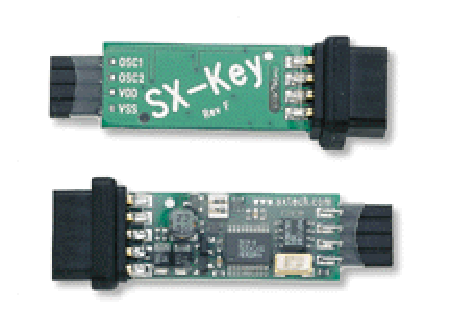
\includegraphics[width=277pt]{sx-key_m.eps}
  \caption{Der SX-Key}
  \label{cr_sx_key}
\end{figure}

Die Debugfunktion erm�glicht die Ausf�hrung von
Programmen schrittweise zu verfolgen und dabei die Registerinhalte zu �berwachen. Desweiteren k�nnen bestimmte Register oder gar Bits formatiert (als bin�re,
hexadezimale oder dezimale Zahl) angezeigt werden. 

\begin{figure}
  \center
  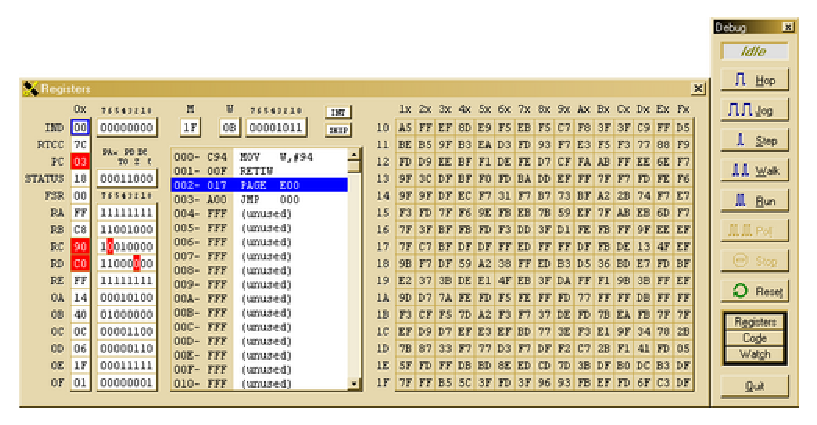
\includegraphics[width=400pt]{regs_dbug_500.eps}
  \caption{Registerfenster mit Debugleiste}
  \label{cr_sx_exe}
\end{figure}

\subsection{Funktionsweise eins SX52 Assemblerprogramms}
Im folgenden wird die Funktionsweise eines SX52 Assemblerprogramms grob umrissen, um eine Verst�ndniss der folgenden Erkl�rungen zuerm�glichen.
Ich gehe davon aus, das Begriffe wie Akkumulator,Clock (oder auch Zeitgeber) und Register bereits bekannt sind.

Die Programme des SX52 sind ein einem 64 Kilobyte grossem EEPROM untergebracht. Jedes Byte hat eine L�nge von zw�lf Bit. Ein Byte repr�sentiert eine
Instruktion f�r den Microcontroller. Dabei teilt sich ein solches Byte je nach Befehl in Operationscode und Argumente. Anders als zum Beispiel bei
einmem MIPS Assembler haben die Operationscodes nicht alle die gleiche L�nge. Die Adresse der aktuell auszuf�hrende Zeile entnimmt man dem
Programmz�hler (zu engl. Programm Counter, abgek�rzt PC).

Ein Programm beginnt an der h�chsten Stelle des Speichers, also an der Stelle FFF (Hexadezimal). Dort wird die Einsprungadresse des Hauptprogramms
eingelesen und in den Programmz�hler geschrieben. Die Einsprungadresse wird auch als ,,\footnote{engl.reset: widerherstellen. In diesem Kontext soll
der Anfangszustand des Programms wieder hergestellt werden}reset'' bezeichnet. Der Befehl an der aktuellen Stelle wird eingelesen und, nach dem der Programmz�hler um Eins iteriert
wurde, ausgewertet.

Ein solches Programm k�nnte nun bis zu h�chsten Stelle durchlaufen und dann wieder von der Stelle FFF (hexadezimal) aus zur�ckspringen. In der Praxis wird das jedoch
selten so gehandhabt. Folgende Ereignisse k�nnen den Kreislauf unterbrechen:

\begin{description}
\item[Rollover-Interrupt]
Der \footnote{engl.roll over: �berschlagen, vorne �berkippen; engl. interrupt: die Unterbrechung}Rollover-Interrupt unterbricht das Programm, schreibt
den aktuellen Inhalt des Programmz�hlers, sowie den Akkumulator und die Register \footnote{FSR: File Select Register, enth�lt den Zeiger auf die
Aktuelle Registerbank}FSR und \footnote{}STATUS in ein eigens f�r die Interruptbehandlung vorgesehenes
Register. Danach werden die Befehle ab der Adresse 000 ausgef�hrt bis das Ende des Interrupts durch einen speziellen R�cksprungbefehl angezeigt wird (hier: RETIW
oder RETI). Diese Befehle sorgen nun daf�r, dass der Programmz�hler, der Akkumulator und die Register FSR und STATUS wieder auf die zuvor gespeicherten
werte gesetzt werden. Die Befehle von der Adresse 000 bis zum R�cksprungbefehl werden im folgenden als Interrupt-Routine bezeichnet.
W�hrend eine Interrupt-Routine ausgef�hrt wird, kann kein weiterer Interrupt erfolgen.
\item[SLEEP-Befehl]
Durch den SLEEP-Befehl wird die Clock ausgeschltet und alle den Microcontroller betreffenden Systeme nur noch minimal versorgt. Das Programm h�lt an.
\item[Multi-Input-Wakeup-Interrupt]
Der Multi-Input-Wakeup-Interrupt wir durch ein Signal am Port B ausgel�st. Er bewirkt entweder das ,,aufwachen'' des Microcontrollers, wenn dieser im
SLEEP-Modus war, oder er startet die Interrupt-Routine.
\item[Endlosschleife]
Man kann das erreichen der h�chste Speicherstelle auch durch eine eigene Endlosschleife verhindern, die w�hrend des Programmlaufes nicht verlassen
wird.
\item[Neustart durch ab- und einschalten der Versorgungsspannung]
Nat�rlich kann man den Microcontroller auch aus- und wieder anschalten um das Programm zu unterbrechen.
\end{description}

W�hrend des Programmablaufes werden Daten eingelesen, bearbeitet und ausgegeben. Dies geschieht in den Registerb�nken. Man Unterscheidet im Fall des
SX52 zwischen globalen und zu adressierenden Registerb�nken zu je 16 Byte a acht Bit. Die globalen Register sind jederzeit adressierbar. Sie enthalten
unter anderen das STATUS-Register, das FSR-Register und die Port-Register. Im FSR ( engl. File Select Register, etwa Dateiauswahlregister) stehen die ersten vier Bit der zu
adressierenden Registerbank. Um eine Bank zu adressieren schreibt man entweder die entsprechende Adresse direkt in das FSR-Register oder nutzt den
BANK-Befehl gefolgt von einer drei Bit Nummer, das viert Bit im FSR wird dabei immer auf 0null gesetzt. Um jetz trotzdem die undgeraden Registerb�nke
adressieren zu k�nnen muss der Programmierer das entsprechende Bit im FSR-Register setzten. Diese umst�ndliche handhabe ist auf die Kompatibilit�t mit
dem SX32 zur�ckzuf�hren, der nur acht Registerb�nke zur Verf�gung stehen hat.

\subsubsection{Unterprogrammaufrufe}
Unterprogrammaufrufe werden mittels CALL-Befehl realisiert. Der SX52 enth�lt einen Stapel der Tiefe acht, um Unterprogramme rekursiv aufzurufen.
Beim Aufruf eines Unterprogramms wird die R�cksprungadresse auf den Stack gelegt und der Programmz�hler auf den Wert des CALL-Arguments gesetzt.
Das Argument kann jedoch nur einen Adressraum von 256 Byte ansprechen (Argumentl�nge: neun Bit), drei der restlichen vier Bit f�r eine vollst�ndige
Programmspeicheradresse stehen im STATUS Register das vierte Bit wird auf null gesetzt. F�r die Programmierung bedeutet dies, das mit einem
Unterprogrammaufruf innerhalb einer Programmspeicherseite nur Unterprogramme in der unteren H�lfte aufgerufen werden k�nnen. Weiter unten im Text wird
ein Konzept beschrieben, das diese Einschr�nkung geschickt umgeht.

\subsubsection{Arbeitsregister}
Der SX52 nutzt in der Summe 17 Register zur Verarbeitung von Daten zur Laufzeit. Die Register teilen sich auf in eine globale Bank und 16 indirekt 
adressierbare B�nke. Jede Bank enth�lt 16 Register. F�r die Adressierung der globalen Register sind keine Vorkehrungen n�tig. Um die 16 ,,normalen''
Registerb�nke zu referenzieren schreibt man einfach die Registernummer hin. Die globale Register haben in den vier \footnote{Most Significent Bits:
H�chstwertigen Bits}MSB einen ungeraden Wert stehen, w�hrend f�r die ,,normalen'' Register immer ein gerader Wert in den ersten vier Bit steht.
Steht alo im Bit Nummer vier des Befehlsarguments eine Eins, so werden die Bits 0 bis 3 f�r die Adressierung eines globalen Registers genutzt, sonst 
wird ein Register aus der im FSR spezifizierten Bank entnommen.
Beispiel:
\begin{verbatim}
; W bezeichnet den Akkumulator
MOV  $1A,W ; schreibt den Inhalt von W in das globale register $1A
BANK $60   ; stellt FSR auf Bank sechs
SETB FSR.4 ; stellt FSR auf Bank sieben
MOV  $0A,W ; schreibtden Inhalt von W in das register Nr.$7A
\end{verbatim}
In der Summe stehen dem Benutzer 256 Register plus 15 globale Register zur Verf�gung. Von den globalen Registern sind die ersten f�nf Register f�r
spezielle Aufgaben vorgesehen (unter anderen FSR und STATUS-Register),dann folgen die f�nf I/O-Ports die auch als Register nutzbar sind, und dann
bleiben noch sechs ,,freie'' Register.

\begin{figure}
  \center
  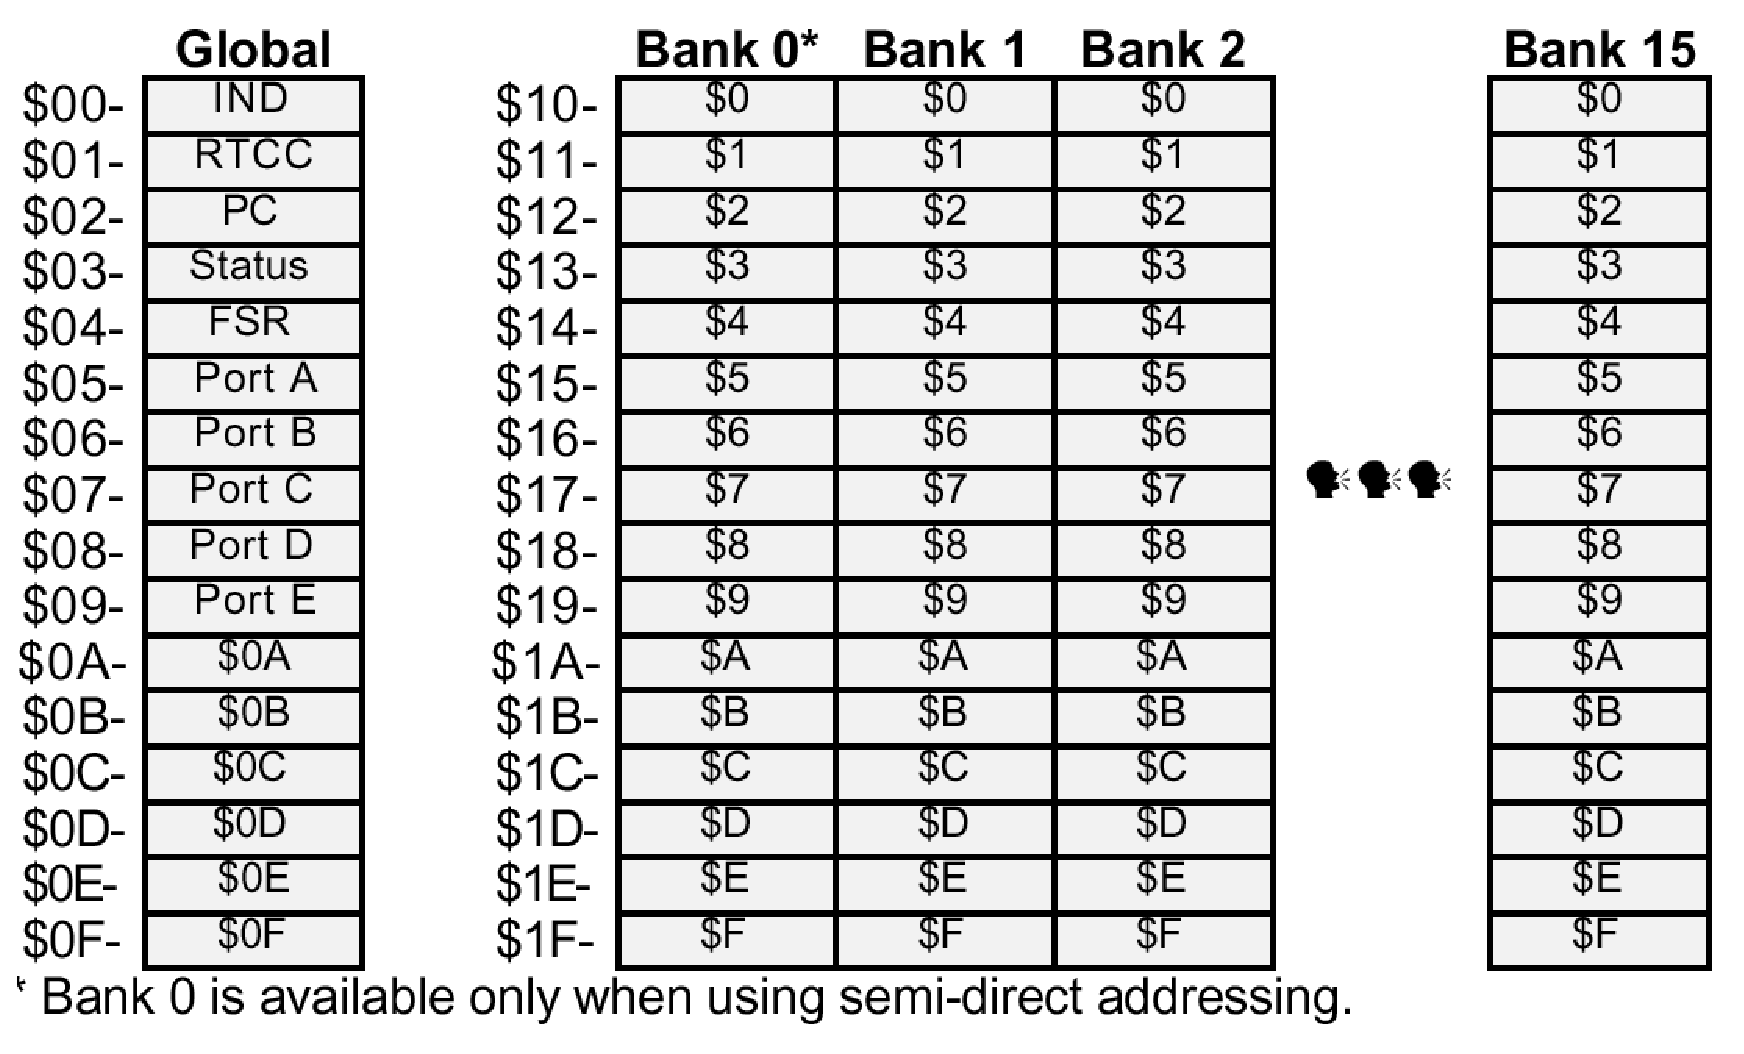
\includegraphics[width=400pt]{register.eps}
  \caption{Aufbau der Registerb�nke im SX52}
  \label{register}
\end{figure}

\section{Assembler-Directiven}

Der zum SX52 gelieferte Assembler stellt eine Reihe von Direktiven zur Verf�gung, die, klug genutzt, die Programmierung vereinfachen.
Eine Dirktive wird nicht zur Laufzeit, sondern bereits vor der Programmierung des Programmspeichers ausgef�hrt. sie dienen zum Beispiel zur
organisation des Programmcodes, zur Benennung von Variablen und Konstanten, oder zur arithmetischen �berpr�fung einiger Programmkomponenten.
Im folgenden werden einige der Direktiven beschrieben und wie sie genutzt werden k�nnen um die Zielsetzungen in der Implementierung zu verfolgen.

\subsubsection{EQU-Direktive}
Mit der EQU-Direktive werden Konstanten oder Registern Namen zugeordnet.
\begin{verbatim}

LED	EQU 	RB.5        ; sechstes Bit auf Port B wird mit LED benannt
FOO	EQU 	$0a         ; das Register 0a wird mit FOO benannt
BAR	EQU 	#%0000_0011 ; die Konstante BAR hat den Wert drei

\end{verbatim}
\subsubsection{ORG-Direktive}
Die ORG-Direktive dient der genauen Platzierung von Programmcode im Programmspeicher. Man definiert eine Speicheradresse zwischen 000 und FFF 
(hexadezimal) an welcher der folgende Programmcode beginnen soll.
\begin{verbatim}

ORG  #000	;der folgende Code wird ab Adresse 000 eingef�gt
# Es folgt die Interrupt-Routine
...

ORG  #200	;der folgende Code steht ab Adresse 200 (hex)
CALL FOO	
MOV  $01, #2	
...

\end{verbatim}
\subsubsection{DS-Direktive}
Die DS-Direktive benennt einen Programmspeicherbereich. Die gr��e des Bereichs in Byte wird als Argumnet �bergeben.
\begin{verbatim}

FOO	DS	1
BAR	DS	2

\end{verbatim}
\subsubsection{MACRO-Direktive}
Ein n�tzliches Werkzeug bei der Speicherorganisation ist die MACRO-Direktive. Programmcode, der in ein Macro eingebunden wird l�sst sich leicht aus dem
Programm entfernen und wieder einsetzen. Diese Eigenschaft erm�glicht es Programmteile genau zu platzieren und so Adressierungsbeschr�nkungen zu
umgehen.
\begin{verbatim}
MACRO 	FOO	; Macro namens FOO

MOV	M,#BAR	; Programmcode

ENDM
.
.
.
ORG	200
FOO		; Macro FOO wird bei 200 (hex) eingef�gt
\end{verbatim}
\subsubsection{\$-Direktive}
Das Dollarzeichen liefert die aktuelle Bank zur�ck.
\begin{verbatim}

FOO EQU $	;FOO enth�lt die aktuelle Bank

\end{verbatim}
\subsection{Konzeption}
\label{Konzeption}

Bei der Konzeption der Module galt es die potentiellen Schwierigkeiten mit Unterprogrammaufruf, Verteilung der Programmteile auf den Speicher, sowie
den Zugriff auf Register f�r den Entwickler m�glichst einfach handhabbar zu machen.
Um dies zu erreichen eignet sich eine Modulstruktur die durch geschicktes Einsetzen der Macro-Direktiven die oben genannten Schwierigkeiten umgeht.

\subsubsection{Modulstruktur}
Man unterteilt jedes Modul in verschiedene Segmente. Begreift man nun ein Assemblerprogramm als Automat mit den Zust�nden Initialisierung,
Hauptfunktion und Interrupt, so werden die einzelnen Segmente an der passenden Stelle eingebunden.
\begin{figure}
  \center
  \includegraphics[width=400pt]{Automat2.eps}
  \caption{Ein Assemblerprogramm als Automat}
  \label{Automat}
\end{figure}
Zus�tzlich Bedarf es f�r die Datenorganisation
noch ein CALL- und ein DATA-Segment. Im folgenden die Segmente im Einzelnen.
\begin{description}
\item[CODE-Segment]
Im CODE-Segment befinden sich die eigentlichen Routinen eines Moduls. Jede Routine beginnt dabei mit einer Einsprungmarke und endet mit einem
R�cksprungbefehl f�r Unterprogramme. Der R�cksprungbefehl setzt die durch einen CALL-Befehl gespeicherten Werte in STATUS-, FSR-Register und
Programmz�hler wieder ein, und f�hrt das Programm von dort an weiter aus.
\item[CALL-Segment]
Das Callsegmnet dient dazu die 256-Byte Grenze des CALL-Befehls zu umgehen. Dieses Segment muss jeweils in den unteren 256-Byte einer
Programmspeicherseite liegen.
Im CALL-Segment werden Funktionsnamen mit den entsprechenden Funktionen im CODE-Segment verkn�pft. Der Trick liegt dabei in der verwendung des
JMP-Befehls. JMP springt an die im Argument �bergebene Stelle in Programmspeicher. Da das Argument des JMP-Befehls neun Bit lang ist, k�nnen die vollen
512 Byte eine Speicherseite referenzeiert werden.
Das CALL-Segment erm�glicht also einen Unterprogrammaufruf ohne die 256-Byte Beschr�nkung bedenken zu m�ssen. Desweiteren f�gt der Assembler noch einen
PAGE-Befehl ein wenn dem CALL ein @ vorangestellt wird, so dass auch dies Beschr�nkung wegf�llt.
\item[DATA-Segment]
Wie bereits oben beschrieben stehen dem Programmierer 256 Register auf verschiedenen B�nken zur Verf�gung. Um mit den Registeradressierungen nicht
durcheinander zu kommen, empfiehlt es sich pro Modul nur auf einer Bank zu arbeiten, die dann ausschlie�lich daf�r reserviert ist.
Die Macros erm�glichen es bei der Programmierung auf Register Adressierung zu verzichten.
Um das zu erreichen definiert man ein Macro in dem platz f�r maximal 16 Register reseviert wird. Man benutzt bei der Programmierung dann nur noch die
Variablen f�r den reservierten Platz. Diese Praxis ist mit der Variablendeklaration in einer Hochsprache vergleichbar, nur das die Typisierung vom
Benutzer und nicht vom Compiler vorgenommen wird.

Um dann die entsprechende Bank zu reservieren, Wird das Macro durch die ORG Direktive an der entsprechenden Stelle eingef�gt. Die erste Instruktion im
Macro weist dann einer Variablen die aktuelle Adresse zu, so da� der Entwickler mit der Kombination BANK-Befehl und eben genannte Variablen die
entsprechende Modulbank referenzieren ohne schon wissen zu m�ssen welche Bank er eigentlich nutzt.
Beipiel
\begin{verbatim}
MACRO 	  FOO	; Macro namens FOO
MEINEBANK $     ; Die aktuelle Bank wird referenziert
VAR1      DS1   ; Ein Register reservieren
VAR2      DS1   ; ...
...
ENDM

ORG	$20
FOO		; Macro FOO wird bei 20 (hex) eingef�gt
                ; enspricht der dritten Bank
\end{verbatim}
\item[INTERRUPT-Segment]
Ben�tigt man f�r ein Modul auch Routinen die durch einen Interrupt ausgel�st werden, so schreibt man den dazu n�tigen Code in ein Macro.
Dieses Macro wird als Interrupt-Segment beschrieben. Die Interrupsegmente schreibt man dann hintereinander an die Adresse 000 (hexadezimal). In den
Interruptsegmenten darf kein Interrupt R�cksprungbefehl stehen. Der muss am Ende der Macroliste stehen um sicherzustellen das alle Segmente ausgef�hrt
werden.
\item[INIT-Segment]
Jedes Modul ben�tigt auch einen Bereich im Initialbereich des Gesamtprogramms zur Initalisierung seiner Variablen. Dazu definiert man zu jedem Modul
ein INIT-Macro. 
\end{description}
Zusammengefasst k�nnte ein Programm nach den oben beschriebenen Konventionen dann wie folgt aussehen:
\small{
\begin{verbatim}
;M O D U L E
; Modul_1

; DATASEGMENT
    MACRO   DATA_MODUL_1
     MEINEBANK $     ; Die aktuelle Bank wird referenziert
     VAR1      DS1   ; Ein Register reservieren
     VAR2      DS1   ; ...
    ENDM
    
; INTERRUPTSEGMENT
    MACRO   INTERR_MODUL_1
    ;Anweisungen die bei Interrupt ausgef�hrt werden sollen
    ENDM
    
; INITSEGMENT
    MACRO   INIT_MODUL_1
    ;Initialisierung der Variablen
    ENDM
    
; CALLSEGMENT
    MACRO   CALL_MODUL_1
     routine_1
     JMP _routine_1 
    ENDM
    
; CODESEGMENT
   MACRO   CODE_MODUL_1
   _routine_1 ;Sprungmarke f�r CALL-Segment
   ; der eigenliche Code
   ...
   ENDM

; Modul_2
...
; CALLSEGMENT
    MACRO   CALL_MODUL_2
     routine_2
     JMP _routine_2
    ENDM
    
; CODESEGMENT
   MACRO   CODE_MODUL_2
   _routine_2 ;Sprungmarke f�r CALL-Segment
   ; der eigenliche Code
   ...
   ENDM
...
; Modul_3
...

;P R O G R A M M
Hier wird jetzt der Programmcode auf den Speicher verteilt

ORG $000
;Interrupt
INTERR_MODUL_1
INTERR_MODUL_2
INTERR_MODUL_3
RETI ;aus Interrupt herausspringen

ORG $500 
main        ;anf�ngliche Einsprungmarke
;Initialisierung
;Interrupt abschalten
...
;allgemeine Konfiguration
...
INIT_MODUL_1
INIT_MODUL_2
INIT_MODUL_3
;Interrupt wieder einschalten
mainprog   ; Hauptteil des Programms
...
@CALL routine_1
...
@CALL routine_2
...
JMP mainprog

ORG $600
CALL_MODUL_1
CALL_MODUL_2
CODE_MODUL_1
CODE_MODUL_2

ORG $800
CALL_MODUL_3
CODE_MODUL_3

\end{verbatim}
}
\subsubsection{Datenaustausch zwischen den Modulen}

Um den Austausch von Daten sicher zu stellen, werden zwei B�nke f�r den Austausch von Daten reserviert. Jedes Modul entnimmt dort seine Eingabewerte und
 legt die Ergebnisse dort wieder ab.

\subsection{Implemetierungen}
Im folgenden werden beispielhaft Module f�r einige Bauelemente beschrieben.
\begin{description}
\item[Serielle Schnittstelle]
Die serielle Datenu"bertragung ist in der Norm RS232 festgelegt.
Danach ko"nnen zwei Computer u"ber die Datenleitungen TxD (Transmit Data) und RxD (Receive Data) miteinander kommunizieren.


Ein Byte wird als Folge von Bits digital gesendet. Zusa"tzlich wird jedem Datenbyte ein Startbit vorangestellt.
Zur U"berpru"fung folgt ein Parita"tsbit und letzlich noch ein Stopbit. Eine Fehleru"berpru"fung (Parity) findet bei der Implementierung in diesem Fall nicht statt.



Die Serielle Schnittstelle nutzt den Interrupt um ein korrektes Timing zu erreichen. Der Befehl RETIW k�rzt den Zeitraum bis zum n�chsten Rollover
Interrupt um den Betrag im Akkumulator W. So l�sst sich die Frequenz relativ genau an den gew�nschte Wert anpassen.
Bei einer Taktfrequenz von 50 MHz ben�tigt ein Zyklus 20 Nanosekunden (Bis auf Sprungbefehle ben�tigt jede Instruktion nur einen
Zyklus).
Die genaue Taktung erreicht man durch den Interrupt.
Bei einer Baudrate von 115200 mu� alle x ns eine Abtastung auf eine eingehendes Signal erfolgen.

Die UART (Universal Asynchronous Receiver / Transmitter) ist ein Chip (Baustein), die zur Kommunikation u"ber eine serielle Schnittstelle beno"tigt wird. Kommunikation bedeute hier Datenaustausch u"ber Input- bzw. Output-Leitungen.
Die UART u"bertra"gt im Modus 8n1 8-Bit-Daten serialisiert in einem Rahmen, der aus einem Start-Bit und einem Stop-Bit besteht. 

 Daraus ergeben sich die Datenu"bertragungsparameter Parita"tsart (even, none, odd, space, mark), Anzahl der Datenbits (5-8), Anzahl der Stopbits (1-2) und die Anzahl der pro Sekunde folgenden Bits (Baudrate; 300-115200). Diese Parameter werden durch entsprechende Software an den seriellen Ein-Ausgabe-Baustein (UART- Universal Asynchroneous Receive and Transmit) u"bermittelt, der die Datenu"bertragung an der seriellen Schnittstelle (COM) steuert. Die Datenu"bertragung ist im wesentlichen von der Leistungsfa"higkeit des UART-Schaltkreises abha"ngig. Insbesondere wird die Baudrate durch verschiedene Schaltkreistypen beschra"nkt (vgl. Bild 8: z.B. UART 8250 bis 19,2 kBaud). 


Die meisten AVR-Typen haben eine Hardware-UART eingebaut. Das Wort UART sagt zuna"chst einmal nur aus, da? 
es sich um einen universellen Sende-Empfa"nger handelt, der asynchron Daten u"bertra"gt. Die asynchrone Datenu"bertragung erfolgt
 im Gegensatz zur synchronen ohne separates Taktsignal. Deshalb ist nur eine Sende- und eine Empfangsleitung sowie eine Masseleitung
  erforderlich. Ein UART-Empfa"nger mu? das eintreffende Signal mit einer mehrfachen Taktferquenz abtasten und so das Taktsignal ru"ckgewinnen. Das setzt ein akkurates Timing beim UART-Sender voraus. Man kann eine UART durchaus als reine Software-Lo"sung realisieren und Bascom bietet diese Mo"glichkeit auch. Aber das kostet sehr viel Rechenzeit (und Programmspeicher), bringt Fehler in der Datenu"bertragungsrate mit sich und la"?t logischerweise keine hohen U"bertragungsraten zu. Bitte achten sie in der Bascom-Hilfe genau darauf, ob sich ein bestimmter Befehl auf die Hard- oder Software-UART bezieht und bringen Sie beides nicht durcheinander.

Datenwort: Die gebra"uchlichste U"bertragungsart fu"r ein Datenwort ist 8N1, also 8 Datenbits, kein (N) Parita"tsbit und 1 Stopbit. Die Hardware-UART des AVR bietet mehr Mo"glichkeiten (z.B. auch 9 Datenbits), aber das will ich hier nicht behandeln. Bascom verwendet standardma"?ig 8N1.


Um eine Frequenz von 115 Baud zu realisieren ben�tigt man eine 4 mal so hohe Abtastfrequenz.

Je nach Fre

Der 


Abtastung 1/4 der Baudrate
Um nun ca. alle 0,008695652 Sekunden ein Signal zu senden 

Alle 256 Zyklen wird ein Rollover Interrupt ausgel�st bei einer Taktfrequenz von 50 MHz sind das 50.000.000 Instr/s = 20 Nano Sekunden pro Instr.

1/50000000=0.000 000 020 Sec -> 20 NanoSek;;  50_000_000 Cyc/sec 460800 Cyc/Sec ==> 108,5069444

TaktFrequenz/4*Baudrate = Anzahl der Instruktionen bis Interrupt ausgel�st werden soll.


Tabelle
Baudraten
von bis 
max = 



115200 Baud -> 115200 Bit/s

460800 bit/s ->0.000_002_17  = ca 2,17 mycroSec

1/115200 => alle 0,000_00868 Sec eine Bit setzten

also ca. alle 0,000_00212 Sec einmal Abtasten

\item[PWM]
Die Puls-Weit-Modulation ist ein Verfahren zur ...


reverse iterations


----Bild von approximierter Kurve------!!!
\item[Speicher]
mini seriell
\item[SPI]
mux 
\item[Sensorik]

R�ckkopplung

\end{description}
\newpage
\section{Fazit}
Die Wahl des Microcontrollers hat sich als gut erwiesen, da sich eine gut handhabbare Programmstruktur erstellen lies. Das dies nicht nur aus der
Sicht eines Informatikers so ist hat die Schulung des M�nchner Projektteams im Mai 2002 gezeigt. Auch in Zukunft wird die Platine dort auch in anderen
f�r den mechatronischen Bereich genutzt werden. Ebenso hat die Arbeit gezeigt wie wichtig der Austausch zwischen den Teammitgliedern und den
beteiligten Disziplinen f�r eine ad�quate Anforderungsl�sung ist.
\section{Ausblick}
Anleitung
C-Compiler
Techn Docu


% Schluss
\chapter{Fazit}\label{fazit_kapitel}
von: Markus Weimer

%\section{Zusammenfassung}
Insgesamt wurde ein Mechatronik-Framework entwickelt, das den
gestellten Anforderungen weitgehend gerecht wird. Teile des
Frameworks, wie die Platine und die darauf aufsetzende Software sind
bereits an der TU M�nchen im Einsatz, wo mechatronische Komponenten
f�r den L�ufer entwickelt werden. Andere Teile wie Kommunikation und
das Fahrerinterface k�nnen derzeit noch nicht eingesetzt werden, da
noch keine mechatronischen Komponenten zur Verf�gung stehen.  Deren
Entwicklungsende wird den Zeitraum der vorliegenden Ausarbeitung
�berschreiten.

Das Autoren-Team wird das Projekt L�ufer weiter begleiten, um auch die
Anwendung der im Rahmen dieser Arbeit erstellten Software zu
unterst�tzen.

Im Rahmen dieser Arbeit wurden allerdings nicht nur die im Hauptteil
beschriebenen Entwicklungen betrieben, sondern auch Erfahrungen in
Bereichen gesammelt, die nur einem Projekt offenstehen.  Diese sollen
im folgenden auch ihren Platz in dieser Ausarbeitung finden.

\begin{description}
\item[Gewinnung von Partnern] Das Projekt L�ufer setzt in seiner
  gesammten Entwicklung sehr stark auf die Zusammenarbeit mit externen
  Partnern aus Industrie und Forschung.  Dies stellt zum einen die
  praktische Umsetzbarkeit der angedachten und dem Partner
  vorgestellten Entwicklung sicher, erm�glicht aber andererseits auch
  die Nutzung externen Know-Hows.
  
  So reisten zwei der Autoren\footnote{Markus Weimer und Christoph
    Reichenbach} gemeinsam nach Bern, um an der dortigen FH deren
  L�sung f�r eine Mechatronik in einem muskelgetriebenen Fahrzeug
  kennenzulernen.  Aus den dortigen Gespr�chen folgten ma�gebliche
  Design-Entscheidungen f�r die Kommunikationsstruktur des L�ufers. Im
  fr�hen Stadium des Projektes reisten die selben Personen nach
  Saarbr�cken, um dort mit Spezialisten der Firma HighTec �ber die
  M�glichkeiten einer Verbindung zwischen PDA und CANBus zu sprechen.
  
  Sp�ter besuchten wiederum zwei der Verfasser dieser
  Arbeit\footnote{Markus Weimer und Christian R�diger} die Firma SHARP
  in Hamburg.  In einem Gespr�ch mit den dort f�r mobile Endger�te
  zust�ndigen Managern gelang es, SHARP als weiteren Industriepartner
  zu gewinnen. Dies war und ist f�r das Projekt als ganzes ein
  wichtiger Erfolg, da SHARP evtl. die Versorgung des Projektes mit
  PDAs f�r die Nullserie leisten wird. Bei Kosten um die 600Euro je
  PDA ist dies ein nicht unerheblicher Posten bei der Frage, ob die
  Nullserie von zehn Fahrzeugen realisierbar ist.
  
\item[Interdisziplin�re Zusammenarbeit] Auch dies ist eine der St�rken
  des Projektes. Das Mechatronik-Team stie� als bisher letztes zum
  L�ufer-Team, in dem sich bis zu diesem Zeitpunkt haupts�chlich
  Maschinenbauer und Designer befanden.  Anders als in anderen
  Bereichen wird im Projekt die Unterschiedlichkeit nicht als
  Handicap, sondern als Chance verstanden.  Jedes Mitglied des
  Projektes kann sich der Unterst�tzung durch andere in deren
  jeweiligem Fachgebiet sicher sein.
  
  So erstellte z.B. der Designer des Projektes Farbschema und
  Layoutvorlagen f�r die CeBIT-Demo (s.u.). Andererseits erstellte
  Markus Weimer f�r die Webseite des Projektes einige interaktive
  Elemente\footnote{z.B. ein Kontakt-Formular} und gab Hinweise zur
  technischen Realisierung der Webseite.  Diese Zusammenarbeit der
  unterschiedlichen Fakult�ten hat auch im Bereich der Mechatronik
  L�sungen erm�glicht, die ohne Sie nicht denkbar gewesen w�ren.
  
\item[Messen] F�r die Industriepartner des L�ufers ist es nat�rlich
  von besonderem Interesse, sich mit dem L�ufer der interessierten
  �ffentlichkeit zu pr�sentieren.  Dies ist vor dem Hintergrund zu
  sehen, da� einiger der Partner im L�ufer mit Technologien arbeiten,
  die so noch nicht kommerziell erh�ltlich sind, oder nur einem sehr
  kleinen Kreis von Spezialisten bekannt sind.  Auf Messen k�nnen sich
  die Industriepartner mit dem L�ufer einen wahren Publikumsmagneten
  auf den Stand stellen, um an Ihm die eigene Technologie zeigen zu
  k�nnen.
  
  F�r das Projekt stellen Messen zum einen eine Herausforderung dar,
  da der L�ufer zum Beginn einer solchen in einem pr�sentablen Zustand
  sein mu�.  Zum anderen bergen die Messen aber auch sehr gro�e
  Chancen in sich, Kontakte zu weiteren interessanten Partnern aus
  Industrie, Forschung und Politik zu kn�pfen.
  
  Das Mechatronik-Team hatte zusammen mit dem Projekt L�ufer die
  Gelegenheit, sich auf der CeBIT 2002 auf dem Stand von IBM zu
  pr�sentieren.  W�hrend dieser Messe wurden erste Kontakte zu SHARP
  (s.o.) und auch zur C't (s.u.) aufgebaut. SHARP hat mittlerweile
  auch einen PDA f�r die Entwicklung zur Verf�gung gestellt.
  
\item[Medien] Ein Fahrzeug wie der L�ufer erregt nat�rlich ein
  gewisses Interesse der �ffentlichkeit und damit ebenfalls das der
  Medien.  Im Rahmen des Projektes sind so schon einige
  Ver�ffentlichungen der Projektarbeit zustande gekommen.
  
  Das Mechatronik-Team hatte im Rahmen des Projektes ebenfalls die
  Gelegenheit, sich einem breiteren Publikum zu pr�sentieren. So z.B.
  in \cite{artikel}. Auch wurden Kontakte zum Computermagazin c't
  gekn�pft.

\end{description}


Insgesamt hat das Projekt dieser Arbeit einen spannenden und
interessanten Rahmen gestellt, auch wenn es durch seinen aktiven
Charakter oftmals das Ziel dieser Arbeit neu definierte. Es bleibt zu
hoffen, das die Universit�tsausbildung in Deutschland zuk�nftig mehr
Studenten die Chance auf ein solches Umfeld bieten kann.



%\newpage
%\section{Ausblick}


% Das Literaturverzeichnis
\bibliography{master}

\end{document}
